%\documentclass[english,twoside]{article}
\documentclass[english,twoside]{labmanual} %labmanual.cls is a modified version of article.cls, 
                                                                     %tweaked to handle \part{} differently

\input{../../131/StudentGuideModule1/labmanual_formatting_commands} %all general latex packages, commands, and definitions now here.

%The \includeonly line below is a great way to save time so you don't always have to compile the WHOLE latex document, if for instance you've only made changes to a single lab.  If you want to compile more than two labs, the syntax is \includeonly{lab1,lab2,lab3} with no spaces after the commas.
%The master.pdf produced will have only the title page, TOC, and that single lab, though the other lab names will appear in the TOC.
%\includeonly{work_power}

%Use the following line to override all of the 1's and 0's in the \includelab statements below
\includealllabstrue

%\renewcommand{\section}{\cleardoublepage\NoExtraPageSection} %Makes each lab start on odd numbered page (right hand side).

\makeindex
\begin{document}



\title{Physics For Doing!\\
Activities for Physics 125}

\author{Emory F. Bunn, 
Mirela Fetea\footnote{Current address: Germanna Community College, Fredericksburg, VA}, 
Gerard P. Gilfoyle, Henry Nebel, \\
Philip D. Rubin\footnote{Current address: Department of Physics, George Mason University, Fairfax, VA}, 
Jack Singal, Matthew L. Trawick, 
and Michael F. Vineyard\footnote{Current address: Department of Physics, Union College, Schenectady, NY}\\[4pt]
Department of Physics, University of Richmond, VA \\[4pt]
%$^2$Department of Physics, George Mason University, Fairfax, VA \\[4pt]
%$^3$Department of Physics, Union College, Schenectady, NY \\[4pt]
%$^4$Germanna Community College, Fredericksburg, VA 22408
}

\maketitle

\vspace{0.8 in}

%\begin{abstract}

\begin{center}
\large{\textbf{Welcome to Physics 125!}}
\end{center}

The exercises in this manual have been developed to support an investigative
physics course that emphasizes active learning. 
%The units are made up of activities designed to guide your investigations in the laboratory. 
Your written work will consist primarily of documenting
your class activities by filling in the entries in the spaces provided
in the units. The entries consist of observations, derivations, calculations,
and answers to questions. Although you may use the same data and graphs
as your partner(s) and discuss concepts with your classmates, all
entries should reflect your own understanding of the concepts and
the meaning of the data and graphs you are presenting. Thus, each
entry should be written in your own words. It is very important
to your success in this course that your entries reflect a sound understanding
of the phenomena you are observing and analyzing. 

Some of these units
have been taken from the Workshop Physics project at Dickinson College
and the Tools for Scientific Thinking project at Tufts University
and modified for use at the University of Richmond. Others have been
developed locally. 
We wish to acknowledge the support we have received for this project
from the University of Richmond and the Instrumentation and Laboratory
Improvement program of the National Science Foundation. Also, we would
like to thank our laboratory directors for their invaluable technical
assistance.
%\end{abstract}


\newpage
\
\thispagestyle{plain}

\newpage
\
%\setcounter{page}{2} %changed from 1 to 2 on 6/9/15 by MT.  The reason is that in the circuit labs, the odd pages need to be on the right (the fronts of each sheet of paper) and the even pages need to be on the left.  This is critical, because these labs have some pages that are meant to be cut out with scissors, so the backs have to be left blank.  This is done by using the \cleardoublepage command, which requires that the odd/even pages not be reversed from the usual.




\setcounter{tocdepth}{1}\tableofcontents{}

%use \includelab[1] to include, or \includelab[0] to exclude.  Can be overridden with \includealllabstrue
%--------------------------------------------
\part{Kinematics}

\includelab{1}{measuring} %teeny changes from 131(?)
\includelab{0}{walking_speed} %131 equivalent
\includelab{0}{converting_units} %131 equivalent
\includelab{1}{measurement} %131 equivalent
\includelab{0}{measurement_length} %131 equivalent
\includelab{0}{determining_pi} %131 equivalent
\includelab{0}{measurement_uncertainty} % different from 131.  (Activity 4)
\includelab{1}{position} %131 equivalent
\includelab{1}{velocity} %131 equivalent
\includelab{1}{relating} %131 equivalent
\includelab{0}{instantaneous_velocity} %131 equivalent, but not suitable for 125 (uses derivatives)
\includelab{1}{changing} %131 equivalent
\includelab{1}{slowing} %131 equivalent
\includelab{0}{equations} %131 equivalent, but not suitable for 125 (significant calculus mentions)
\includelab{1}{grav_freefall} %131 equivalent
\includelab{0}{acceleration} %131 equivalent
\includelab{0}{reaction_time} %131 equivalent
\includelab{0}{tossed_ball} %131 equivalent
\includelab{0}{independence} %131 equivalent
\includelab{0}{ski_jump} %131 equivalent
\includelab{0}{projectile} %131 equivalent
\includelab{0}{circ_motion} %131 equivalent

%--------------------------------------------
\part{Newton's Laws}

\includelab{1}{force1} %131 equivalent (but does say ``derivative'' in one homework problem. fixable.)
\includelab{0}{force2} %131 equivalent
\includelab{0}{combining} %131 equivalent
\includelab{0}{force_mass} %131 equivalent
\includelab{1}{newton} %131 equivalent
\includelab{0}{atwood} %131 equivalent
\includelab{1}{friction} %131 equivalent
\includelab{1}{elec_grav} %131 equivalent
\includelab{1}{momentum} %Significant differences from 131 version, but I think 131 version is okay.  Check this.
\includelab{0}{centripetal} %131 equivalent
\includelab{0}{kepler} %131 equivalent

%--------------------------------------------
\part{Conservation Laws}

\includelab{1}{work_power} %131 equivalent, does include single mention of dW/dt
\includelab{1}{work_kinetic} %131 equivalent, but doesn't seem appropriate for 125 (says ``differentiate'')
\includelab{1}{conservation_mech} %131 equivalent
\includelab{0}{conservative} %131 equivalent, but note reference to ``next semester'' :-)
\includelab{0}{momentum} %131 equivalent, but uses calculus
\includelab{0}{impulse} %131 equivalent, but uses calculus
\includelab{0}{newtons_laws} %131 equivalent, but uses calculus
\includelab{0}{mom_cons} %131 equivalent
\includelab{0}{twod_collisions} %131 equivalent

%--------------------------------------------
%\part{Rotational Motion}

\includelab{0}{ang_lin_displacement}  %131 equivalent
\includelab{0}{rotation} %131 equivalent, but not suitable for 125 (uses derivatives)
\includelab{0}{newtons_2law_rot} %131 equivalent
\includelab{0}{rolling} %131 equivalent
\includelab{0}{moment_inertia}  %131 equivalent
\includelab{0}{ang_mom} %131 equivalent, uses calculus
\includelab{0}{cons_ang_mom} %131 equivalent, uses calculus

%--------------------------------------------
\part{Oscillation, Resonance, and Waves}


\section{Hooke's Law}

Name \rule{2.0in}{0.1pt}\hfill{}Section \rule{1.0in}{0.1pt}\hfill{}Date \rule{1.0in}{0.1pt}

{\noindent \bf Objectives:} \begin{list}{$\bullet$}{\itemsep0pt \parsep0pt}

\item To explore the nature of elastic deformation and restoring forces

\end{list}

\noindent {\bf Introduction} 

There is no such thing as a perfectly rigid body. The stiffest of metal bars can be twisted, bent, stretched, and compressed. Delicate measurements show that even small forces cause these distortions. Under certain circumstances (typically, when the forces are not too large), a body deformed by forces acting upon it will return to its original size and shape when the forces are removed, a capacity known as elasticity. Permanent distortion from large forces is referred to as plastic deformation. In this lab, you will stay within the elastic limit. \\

{\noindent \bf Apparatus:} \begin{list}{$\bullet$}{\itemsep0pt \parsep0pt}

\item two springs and supports \item collection of masses \item 2-meter stick

\end{list}

{\noindent \bf Activity:} \begin{enumerate}

%\item  Record the mass of the two springs.

%\begin{displaymath} m_1 = \hskip50pt  m_2 = \end{displaymath}

\item  Suspend one of the springs from the support. Using the meter stick, observe the position of the lower end of the spring and record the value in the table below.

\item  Hang 100 grams from the lower end of the spring and again record the position of this end.

\item  Repeat 2 with loads of 200, 300, 400, and 500 grams hung from the spring.

\item  Repeat 2, and 3 with the second spring.

\begin{center} \begin{tabular}{||c|c|c||c|c|c||} \hline \hline Mass suspended & Position & Elongation & Mass suspended & Position & Elongation \\ from spring 1 & reading & & from spring 2 & reading & \\ (g) & (m) & (m) & (g) & (m) & (m) \\ \hline \hline 0 & & 0 & 0 & & 0 \\ \hline 100 & & & 100 & & \\ \hline 200 & & & 200 & & \\ \hline 300 & & & 300 & & \\ \hline 400 & & & 400 & & \\ \hline 500 & & & 500 & & \\ \hline \hline \end{tabular} \end{center}

\item Determine the elongation produced by each load.

\item  Plot a graph using the values of the elongation as the abscissas (x values) and the forces due to the corresponding loads as ordinates (y values) for each spring. Make sure you use compatible units. Write the equation for each curve in the space below.

\vskip70pt

\end{enumerate}

\pagebreak

\textbf{Questions:}

\begin{enumerate}
\item What do your graphs show about the dependence of each spring's elongation upon the applied force?\vspace{30mm}

\item List the proportionality constant (including proper units) for each spring in the space below.\vspace{30mm}

\item The slope of each line (the proportionality constant) is known as the force constant, $k$. Which spring has the larger force constant? Express in your own words the physical implications of different size force constants.
\end{enumerate}
  %131 equivalent

\section{Periodic Motion}

Name \rule{2.0in}{0.1pt}\hfill{}Section \rule{1.0in}{0.1pt}\hfill{}Date \rule{1.0in}{0.1pt}

{\bf Objectives }

\begin{itemize}
\item To learn directly about some of the characteristics of periodic motion, namely period, frequency, and amplitude. 
\item To investigate the relationships between position, velocity, acceleration, and force in simple harmonic motion. 
\item To investigate energy in simple harmonic motion.
\end{itemize}
\textbf{Introduction }

Periodic motion is motion that repeats itself. You can see the repetition in
the position-, velocity-, or acceleration-time graphs. The length of time to
go through one cycle and begin to repeat the motion is called the period. The
number of cycles in each second is called the frequency. The unit of frequency,
cycles per second, is given a special name --- Hertz.

\textbf{Motion of a Mass Hanging from a Spring} 

In this unit you will investigate the motion of a mass hanging from a spring.

\textbf{Apparatus} 

\begin{itemize}
\item Large spring 
\item Force probe 
\item Motion detector 
\item Variety of masses 
\item \textit{Science Workshop 750 Interface}
\item \textit{DataStudio} software (Position \& Velocity Graphs application and SHM
application)
\end{itemize}
\textbf{Activity 1: Periodic Motion of a Mass-Spring System} 

(a) Open the \textbf{Position \& Velocity Graphs} application in the \textbf{131 Workshop} menu.
Hang the large spring from the force probe hook with the
large diameter coils down and hang a 200-g mass from the spring. Place the motion detector facing up directly below the spring. Pull the mass downward about 
15 cm, and let go. Adjust the height of the support so that the mass comes no
closer than 0.15 m to the detector. Record data for a few seconds to display
position-time and velocity-time graphs of the motion. Sketch the graphs on the
axes below.

\vspace{0.3cm}
{\par\centering 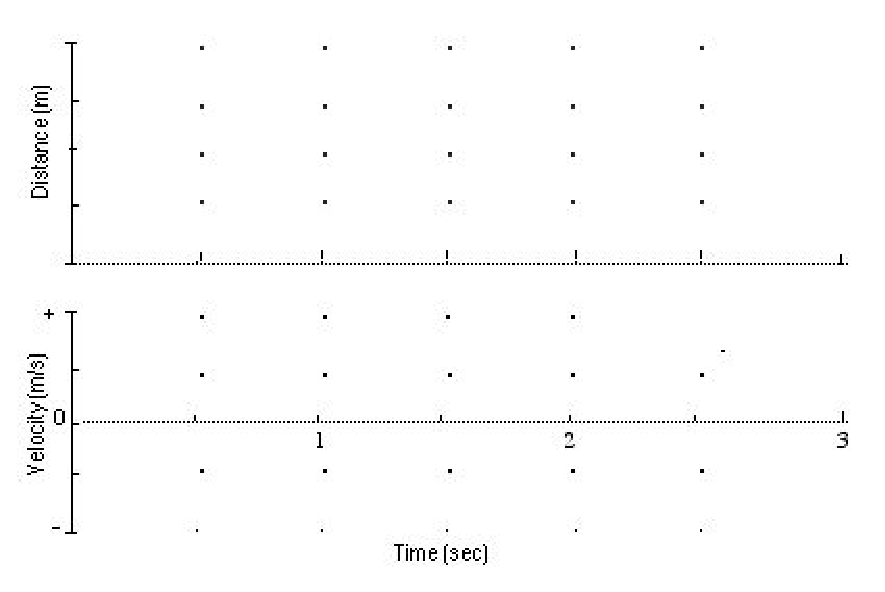
\includegraphics{periodic_motion_fig1.eps} \par}
\vspace{0.3cm}

\textbf{Comment}: Note that when an object returns to the same position, it 
does not
necessarily mean that a cycle is ending. It must return to the same position,
and the velocity and acceleration must also return to the same values in both
magnitude and direction for this to be the start of a new cycle. 

%(b) Label the graphs above with: ``B'' at the Beginning of a
%cycle and ``E'' at the End of the same complete cycle. ``A''
%on each spot where the mass is moving Away from the detector fastest. ``T''
%on each spot where the mass is moving Toward the detector fastest. ``S''
%on each spot where the mass is standing Still. ``F'' where the
%mass is Farthest from the motion detector. ``C'' where the mass
%is Closest to the motion detector.

(b) Do the position and velocity graphs appear to have the same period? Do their
peaks occur at the same times? If not, how are the peaks related in time, i.e. 
what fraction of a period is their phase difference?
\vspace{20mm}

(c) Use the Smart Tool to measure the period of the motion. (For
better accuracy, measure the total time over as many cycles as possible and
divide by the number of cycles.) Record the period here:
\vspace{15mm}

%(e) Using the Smart Tool, determine and record the maximum displacement. Then
%record data with the mass at rest to find the equilibrium position. Draw a straight
%line on your position graph indicating the equilibrium position in terms of
%the distance from the motion detector. Calculate and record the amplitude of
%the motion (the difference between the maximum displacement and the equilibrium
%position).
(d) Calculate the period from
\[T=2\pi \sqrt{\frac{m}{k}.}\]

using the k value determined in the Hooke's Law experiment.
\vspace{15mm}

(e) Calculate the percent difference between your two values.


\newpage

\textbf{Simple Harmonic Motion }

The motion of a mass hanging from a spring that you looked at in Activity 1
is a close approximation to a kind of periodic motion called simple harmonic
motion (sometimes abbreviated SHM).

\textbf{Activity 2: What Factors Determine the Period of the Mass-Spring System? }

What can you do to change the period of the SHM of the mass-spring system? What
will happen to the period if you increase the amplitude? Increase the mass?
Increase the spring constant (use a stiffer spring)?
\vspace{30mm}

\textbf{Activity 3: The Period of SHM and the Amplitude} 

(a) Repeat the procedure of Activity 1, but with a different starting position
(other than 15 cm). (Warning: Do not make the amplitude so large that the mass
comes closer than 0.15 m from the motion detector.) When you have good graphs,
find and record the period and the amplitude using the methods described in
Activity 1. 
\vspace{20mm}

(b) Take ratios of the period and the amplitude of Activity 1 to those determined
here.
\vspace{20mm}

(c) Is there evidence that the period depends on amplitude? (Did the change
in amplitude result in a comparable change in period?) Explain. How does this
compare with your prediction?
\vspace{20mm}

\textbf{Activity 4: The Dependence of the Period of a SHM on the Mass} 

(a) Carefully measure the period for four other masses. Record the masses and
the measured periods in a table in the space below along with the mass and 
period from Activity 1. \textbf{Note:} Add half the mass of the spring to each 
mass value. This accounts for the fact that the theory of SHM neglects the 
mass of the spring.
\vspace{30mm}

(b) Does the period depend on the mass? Does it increase or decrease as mass
is increased?
\vspace{20mm}

(c) Determine the mathematical relationship between the period $T$ and the mass
$m$ by finding a function that fits the data. Do this by using $Excel$ to plot a graph of $T$ vs $m$ and fitting the data with a power function. Write the equation that provides the best fit to the data in the space below.
\vspace{20mm}

\textbf{Comment:} You should have found that $T$ is independent of amplitude and proportional to \( \sqrt{m} \). The actual expression for the period is
\[T=2\pi \sqrt{\frac{m}{k}.}\]


\textbf{Velocity, Acceleration, Force and Energy }

In this investigation you will look more carefully at the distance, velocity
and acceleration graphs for simple harmonic motion. You will also look at the
force graph, and will examine the energy associated with simple harmonic motion.

\textbf{Activity 5: Determination of the Spring Constant }

Measure the distance the spring stretches for four different masses and use
these data to determine the spring constant, $k$, as you did in the Hooke's Law experiment. Record your data and the result for $k$ in the space below.
\vspace{40mm}

\textbf{Activity 6: Velocity, Acceleration, and Force for SHM} 

(a) Consider the motion you looked at in Activity 1 when the mass was 200 g
and the initial position was 15 cm. Sketch the position and velocity graphs
that you observed on the axes below using dashed lines.

\vspace{0.3cm}
{\par\centering 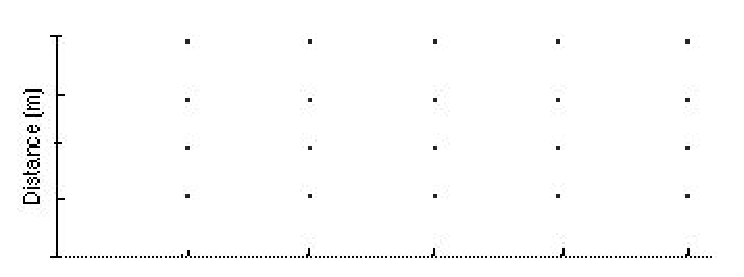
\includegraphics{periodic_motion_fig2.eps} \par}
\vspace{0.3cm}

\vspace{0.3cm}
{\par\centering 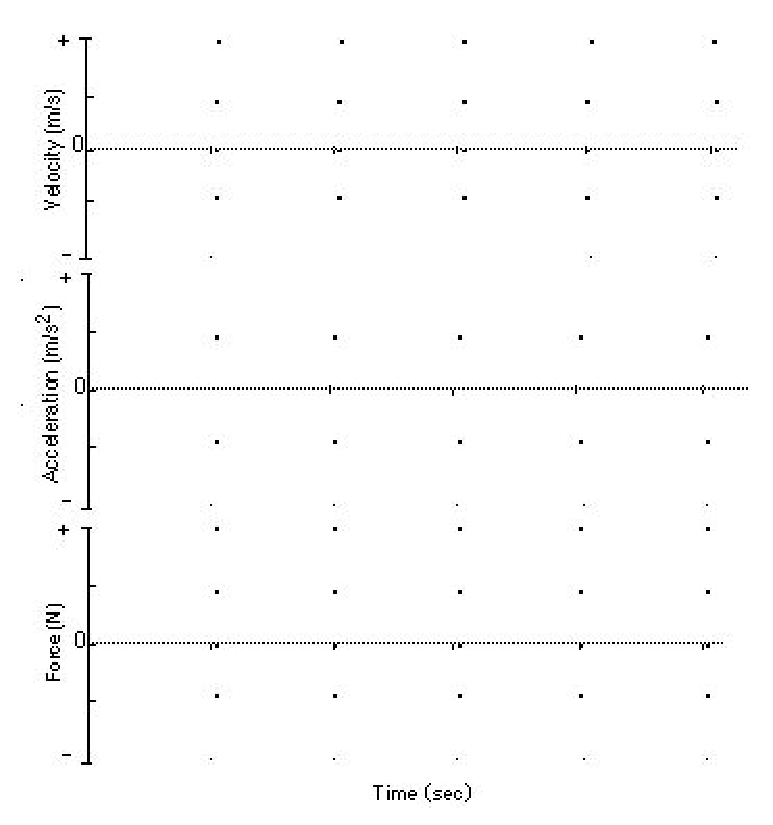
\includegraphics{periodic_motion_fig3.eps} \par}
\vspace{0.3cm}

(b) Based on what you know about the relationships between velocity, acceleration,
and force, use dashed lines to sketch your predictions for the acceleration
and force graphs.

(c) Suspend the 200-g mass from the spring and open the \textbf{SHM} application in the \textbf{131 Workshop} menu. Start
the mass oscillating with an amplitude of 15 cm and record data for a few seconds. When you have obtained good graphs, sketch the results on the above axes using solid lines. Print your graph and attach to this unit.

(d) When the mass is at its maximum distance from the detector, is the velocity
maximum, minimum or some other value according to your graphs? Does this agree
with your predictions? Does this agree with your observations of the oscillating
mass? Explain.
\vspace{15mm}

(e) When the mass has its maximum positive velocity, is its distance from the
detector maximum, minimum, the equilibrium value or some other value according
to your graphs? What about when it reaches maximum negative velocity? Does this
agree with your predictions? Does this agree with your observations of the oscillating
mass? Explain. 
\vspace{20mm}

(f) According to your graphs, for what distances from the detector is the acceleration
maximum? For what distances is the acceleration zero? What is the velocity in
each of these cases?
\vspace{20mm}

(g) Compare the force and acceleration-time graphs. Describe any similarities.
Does the force graph agree with your prediction?
\vspace{20mm}

(h) From your graphs, what would you say is the relationship between force and
acceleration? 
\vspace{20mm}

(i) Compare the force and distance(position)-time graphs. What would you say
is the relationship between force and position? 
\vspace{20mm}

\textbf{Activity 7: Energy of a Mass Undergoing SHM }

Now use the graphs from the last activity to examine the energy relationships
in simple harmonic motion. To do this you will need to draw a horizontal line through the equilibrium position on the position vs time graph as you did in Activity 1. $x$ values must be measured relative to this equilibrium position.

(a) At what points is the kinetic energy of the mass zero? Label these points
on your distance and velocity graphs above with a K.

(b) Calculate the elastic potential energy due to the spring at one of these
points. Label the point you use on your velocity and distance graphs with a
1. Use $U = {1\over 2}kx^{2}$, where 
$x$ is the distance from the equilibrium position
and $k$ is the force constant of the spring, 
which you have already measured. Use
the Smart Tool to measure $x$. Show your data and calculations in the space below. 
\vspace{20mm}

(c) At what points is the potential energy zero? Label these points with a P
on your distance and velocity graphs.

(d) If you measured the kinetic energy at one of these points, what would you
expect its value to be? Explain.
\vspace{20mm}

(e) Check your prediction. Calculate the kinetic energy at one of these points.
Label the point you use on your velocity graph with a 2. Use 
$K = {1\over 2} mv^{2}$.
Use the Smart Tool to determine $v$. Show your data and calculations in the space
below.
\vspace{20mm}

(f) Did your calculated kinetic energy agree with your prediction?
\vspace{20mm}

(g) If you calculated the potential and kinetic energies at a point where neither
of these was zero, what would you expect the total energy to be? Explain.
\vspace{20mm}

(h) Check your prediction. Pick a point where the mass has both kinetic and
potential energy and calculate them both. Label this point on your distance
and velocity graphs with a 3. Show your calculations.
\vspace{40mm}

(i) Does your result agree with your prediction? Does it appear that energy
is conserved? Explain.

  %131 equivalent

\section{The Period of a Pendulum}

Name \rule{2.0in}{0.1pt}\hfill{}Section \rule{1.0in}{0.1pt}\hfill{}Date \rule{1.0in}{0.1pt}

{\noindent \bf Objectives:} \begin{list}{$\bullet$}{\itemsep0pt \parsep0pt}

\item Study the influences on the motion of a simple pendulum \item Calculate the acceleration due to gravity from measurements of the period and length of a simple pendulum

\end{list}

{\noindent \bf Introduction:}

\noindent The period of a simple pendulum is related to its length and the acceleration due to gravity according to the relationship:
\[
T=2\pi \sqrt{\frac{L}{g}}.\qquad [Eq.\: 1]\]

\noindent $T$ is the period, $L$ is the length, and $g$ is the gravitational acceleration. This assumes the oscillations are small. Let's check this prediction experimentally. \\

{\noindent \bf Apparatus:} \begin{list}{$\bullet$}{\itemsep0pt \parsep0pt}

\item string attached to stand \item collection of masses \item stop watch \item meter stick

\end{list}

{\noindent \bf Activity:} \begin{enumerate}

\item With $L$ = 1.0 m, place a 1-kg mass at the end of your pendulum. Time twenty-five (25) oscillations of amplitude not greater than 10 degrees. The period is the total time divided by the number of oscillations. Calculate the period and enter the relevant data into the table below.

\item Repeat 1 for masses of 500 g, 200 g, 100 g, 50 g, and 20 g.

\begin{center} \begin{tabular}{|c|c|c|c|c|c|} \hline Trial No. & Mass & Length[$L$] & No. of & Total Time & Period[$T$] \\ & (kg) & (m) & Oscillations & (s) & (s) \\ \hline \hline 1 & & & & & \\ \hline 2 & & & & & \\ \hline 3 & & & & & \\ \hline 4 & & & & & \\ \hline 5 & & & & & \\ \hline 6 & & & & & \\ \hline \end{tabular} \end{center}

\item With the 200-g mass, fix the length $L$ to be 1.5 m. Time twenty-five (25) oscillations of amplitude not more than 10 degrees. Calculate the period and period squared, and enter the relevant data into the table below.

\item Repeat 3 for pendulum lengths of 1.0, 0.7, 0.4, 0.25, and 0.15 meters.

\begin{center} \begin{tabular}{|c|c|c|c|c|c|c|} \hline Trial No. & Mass & Length[$L$] & No. of & Total Time & Period[$T$] & $T^2$ \\ & (kg) & (m) & Oscillations & (s) & (s) & (s$^2$) \\ \hline \hline 7 & & & & & & \\ \hline 8 & & & & & & \\ \hline 9 & & & & & & \\ \hline 10 & & & & & & \\ \hline 11 & & & & & & \\ \hline 12 & & & & & & \\ \hline \end{tabular} \end{center}

\item Plot $T$ as a function of mass from the first set of data and $T^2$ as a function of $L$ from the second set of data on SEPARATE graphs. NOTE: Be sure the $T$ versus mass graph contains the origin. (If you don't know how to do this, consult your instructor.) Fit the data and determine the slopes of the lines of each graph. Be sure to include UNITS with each slope. Print both graphs and include with this unit.

\end{enumerate}

\vspace{10pt}

slope: period versus mass \rule{1.5in}{0.2pt}

\vspace{10pt}

slope: period$^2$ versus length \rule{1.5in}{0.2pt}

\vspace{10pt}

{\noindent \bf Questions:}

\begin{enumerate}
\item Interpret the slope of the period versus mass line: What is the relationship
between mass and period? How does the period depend on the mass? \vspace{20mm}

\item Interpret the slope of the period$^2$ versus length line: What is the relationship
between length and period? How does the period depend on pendulum length? \vspace{20mm}

\item If the length of the pendulum were $\frac{1}{16}$ its original length, by how
much would its period change? \vspace{20mm}

\item Using the relationship between length and period (equation 1) and the slope you measured for the $T^2$ vs $L$ graph, determine the acceleration due to gravity $g$.  Calculate the percent difference between your value and the accepted value of [9.8 $\frac{\rm m}{\rm s^2}$].
\end{enumerate}
 %131 equivalent
%
\section{Air Column Resonance\footnote{
Adapted from \underbar{Experiments in Physics}, 6th ed., B. Cioffari, D. Edmonds,
Jr. D. C. Heath and Co., 1978.
}}

Name \rule{2.0in}{0.1pt}\hfill{}Section \rule{1.0in}{0.1pt}\hfill{}Date \rule{1.0in}{0.1pt}



{\noindent \bf Objectives:} \begin{list}{$\bullet$}{\itemsep0pt \parsep0pt}

\item Measure the wavelengths in air of sound waves of different frequencies.

\item Determine the velocity of sound in air.

\end{list}

\noindent {\bf Introduction} 

The speed
of a wave is directly proportional to both the frequency of vibration and the length of the wave,

\begin{equation} v = \lambda f \end{equation}

\noindent A tuning fork held over the open end of a tube will send air disturbances (compressions and rarefactions) down the length of the tube. As the medium changes at the other end of the tube, the disturbances will be reflected. Should these reflections be in phase with the waves generated by the tuning fork, resonance occurs, that is, the disturbances reinforce one another and produce a louder sound.

\noindent In order that the tube resonate, the frequency of the vibrating air must coincide with the natural frequency of the tube (which may be its fundamental or one of its overtones). For a tube like the one used in this experiment, which is closed at the opposite end, this requirement is met if the tube length is an odd number of quarter wavelengths of the sound waves produced by the fork ($l = \lambda/4, 3 \lambda/4, 5 \lambda/4$, etc., where $l$ is the length of the tube and $\lambda$ is the wave length of the sound). Note that if the length of the tube is gradually increased while the fork is vibrating, the distance between successive resonance positions is $\lambda/2$. \\

\noindent {\small {\bf Note:} Due to edge effects at the open end of a tube, the length of the wave depends on the radius of the opening. Thus, $l_{eff} = l + 0.6r$, where $l_{eff}$ is the \textit{effective} length, $l$ is the length measured, and $r$ is the tube radius.} \\

\noindent By raising and lowering a brass tube inserted vertically into a larger plastic tube filled with water, column length may be varied. The (effective) length at resonance gives the wavelength; the tuning fork frequency gives the sound frequency. Formula 1 then gives the velocity. \\

{\noindent \bf Apparatus:} \begin{list}{$\bullet$}{\itemsep0pt \parsep0pt}

\item resonance tube setup \item 2 tuning forks of different pitches \item meter stick \item rubber hammer \item thermometer

\end{list}

{\noindent \bf Activity:} \begin{enumerate}

\item You will first determine the shortest tube length for resonance. Do this as follows: Start the tuning fork vibrating by striking it gently with the rubber hammer. Be sure the brass tube is in its lowest position and the fork extends over the open end in such a manner that the prongs vibrate vertically.

\item Slowly raise the brass tube until the first position of resonance is reached.

\item Measure and record the distance from the open end of the tube to the water level in the plastic tube.

\item Raise the tube until the next position of resonance is reached and measure and record the distance as before.

\item Continue with a third position of resonance.

\item Repeat 1- 5 with the same fork twice more for a total of three independent measurements of resonance positions.

\item Repeat 1- 6 with a second tuning fork of a different frequency.

\end{enumerate}

\vskip35pt

\noindent {\Large{\bf DATA}} \\

\noindent Room Temperature ($^\circ$C) \hrulefill \ \  Tube radius (m) \hrulefill

\begin{center} \begin{tabular}{||c|c|c|c|c|c|c|c|c|c|c|c|c|c|c||} \hline \hline Tuning Fork & \multicolumn{4}{|c|}{First Position of} & \multicolumn{4}{|c|}{Second Position} & \multicolumn{4}{|c|}{Third Position of} & Wave- & Velocity of \\ Frequency, & \multicolumn{4}{|c|}{Resonance, m} & \multicolumn{4}{|c|}{of Resonance, m} & \multicolumn{4}{|c|}{Resonance, m} & length, & Sound in \\ \cline{2-13} Hz & 1 & 2 & 3 & Ave. & 1 & 2 & 3 & Ave. & 1 & 2 & 3 & Ave. & m & air, m/s \\ \hline \hline &&&&&&&&&&&&&& \\ \hline &&&&&&&&&&&&&& \\ \hline \hline \end{tabular} \end{center}


{\noindent \bf Analysis:} \begin{enumerate}

\item For each (effective) length of resonating air column, calculate the average of the three readings.

\item For each tuning fork, determine the value of the wavelength of its sound wave in air from the average lengths of the resonating column.

\item For each tuning fork, use the tuning fork frequency and the wavelength determined to calculate the velocity of sound in air.

\item Average your two values to determine your experimental velocity of sound in m/s: \ \ \  \rule{2cm}{1pt}

\item The velocity of sound in air at $0^\circ$C is 331.4 m/s.  The temperature dependence of sound velocity in air is given by $v(T) = 331.4 + 0.6T$, where $T$ is in $^\circ$C and $v$ is in m/s. Calculate an ``accepted'' value of the velocity of sound in air from this formula.

\vskip35pt

\item What is the percent difference between your experimental result and the ``accepted'' value?

\end{enumerate}

\vskip35pt

\noindent{\bf Questions:} 

\begin{enumerate}
\item Suppose that, in this experiment, room temperature had been lower. How would
the length of the resonating air column have changed? Explain. \vspace{20mm}

\item How would an atmosphere of hydrogen affect the pitch of a tuning fork? Explain.\vspace{20mm}

\item A tuning fork rated at 128 vibrations per second is held over a resonance tube.
What are the two shortest distances at which resonance will occur at a temperature
of $20^\circ$C?\vspace{20mm}

\item The first resonance of a tube is found to occur when the position of the water
line below a vibrating tuning fork is at 10 cm. A second resonance is found
at 26 cm. What is the frequency of the tuning fork? (Take the air temperature
to be 20$^\circ$C.)
\end{enumerate}
 %131 equivalent
%\section{Music to Our Ears: Standing Waves in Strings}

Name \rule{2.0in}{0.1pt}\hfill{}Section \rule{1.0in}{0.1pt}\hfill{}Date
\rule{1.0in}{0.1pt}

\textbf{Aim:}
\begin{itemize}
\item  to study the natural modes of vibration of a stretched string
\end{itemize}

\textbf{Equipment:}
\begin{itemize}
\item  string vibrator and power supply
\item  inelastic braided string
\item  2 clamps
\item  superpulley
\item  mounting rod for the superpulley
\item  mass and hanger set
\item  balance
\item  tape measure
\end{itemize}


How do we make musical sounds? To make a sound , we need something that vibrates. If we want to make musical notes you usually need the vibration to have an almost constant frequency: that means stable pitch. We also want a frequency that can be easily controlled by the player. In electronic instruments this is done with electric circuits or with clocks and memories. In non-electronic instruments, the stable, controlled vibration is produced by a standing wave. Here we discuss the way strings work. This is also a good introduction for studying wind instruments, because vibrating strings are easier to visualise than the vibration of the air in wind instruments, but the math is very similar.  

\textbf{Introduction}

Waves are oscillations in an elastic medium:

\begin{itemize}
\item  your own vocal cords (the medium) vibrating as air is forced over them by your lungs; 
\item  a stretched string (the medium) on a musical instrument vibrating as it is bowed, hammered or plucked; 
\item  pressure oscillations in a column of air (the medium) in a wind instrument, organ pipe or your own oral and nasal cavities.
\end{itemize}

In each case the medium has an equilibrium state, and when displaced or otherwise perturbed from that state, experiences a force which tends to restore it to equilibrium. For small perturbations, the restoring force is proportional to the displacement and the medium becomes a simple harmonic oscillator.

There are also waves that do not require a medium, namely electromagnetic waves, which will be discussed later in the course.

\textbf{Background}

Standing waves (stationary waves) are produced by the interference of two traveling waves, both of which have the
same wavelength, speed and amplitude, but travel in opposite directions through the same medium. The necessary conditions for the production of
standing waves can be met in the case of a stretched string by having waves set up by some vibrating body, reflected at the end of the string and then interfering with the oncoming waves.

One characteristic of every standing wave pattern is that there are points along the medium which appear to be standing still. These points, sometimes described as points of no displacement, are referred to as nodes. There are other points along the medium which undergo vibrations between a large positive and large negative displacement. These are the points which undergo the maximum displacement during each vibrational cycle of the standing wave. In a sense, these points are the opposite of nodes, and so they are called antinodes. A standing wave pattern always consists of an alternating pattern of nodes and antinodes. When a standing wave pattern is established in a medium, the nodes and the antinodes are always located at the same position along the medium; they are "standing still." It is this characteristic which has earned the name "standing wave."

A stretched string has many natural modes of vibration (three examples are shown below). If the string is fixed at both ends then there must be a node at each end. It may vibrate as a single segment, in which case the length ($L$) of the string is equal to 1/2 the wavelength ($\lambda $) of the wave. It may also vibrate in two segments with a node at each end and one node in the middle; then the wavelength is equal to the length of the string. It may also vibrate with a larger integer number of segments. In every case, the length of the string equals some integer number of half wavelengths.

\vspace{0.3cm}
\begin{center}
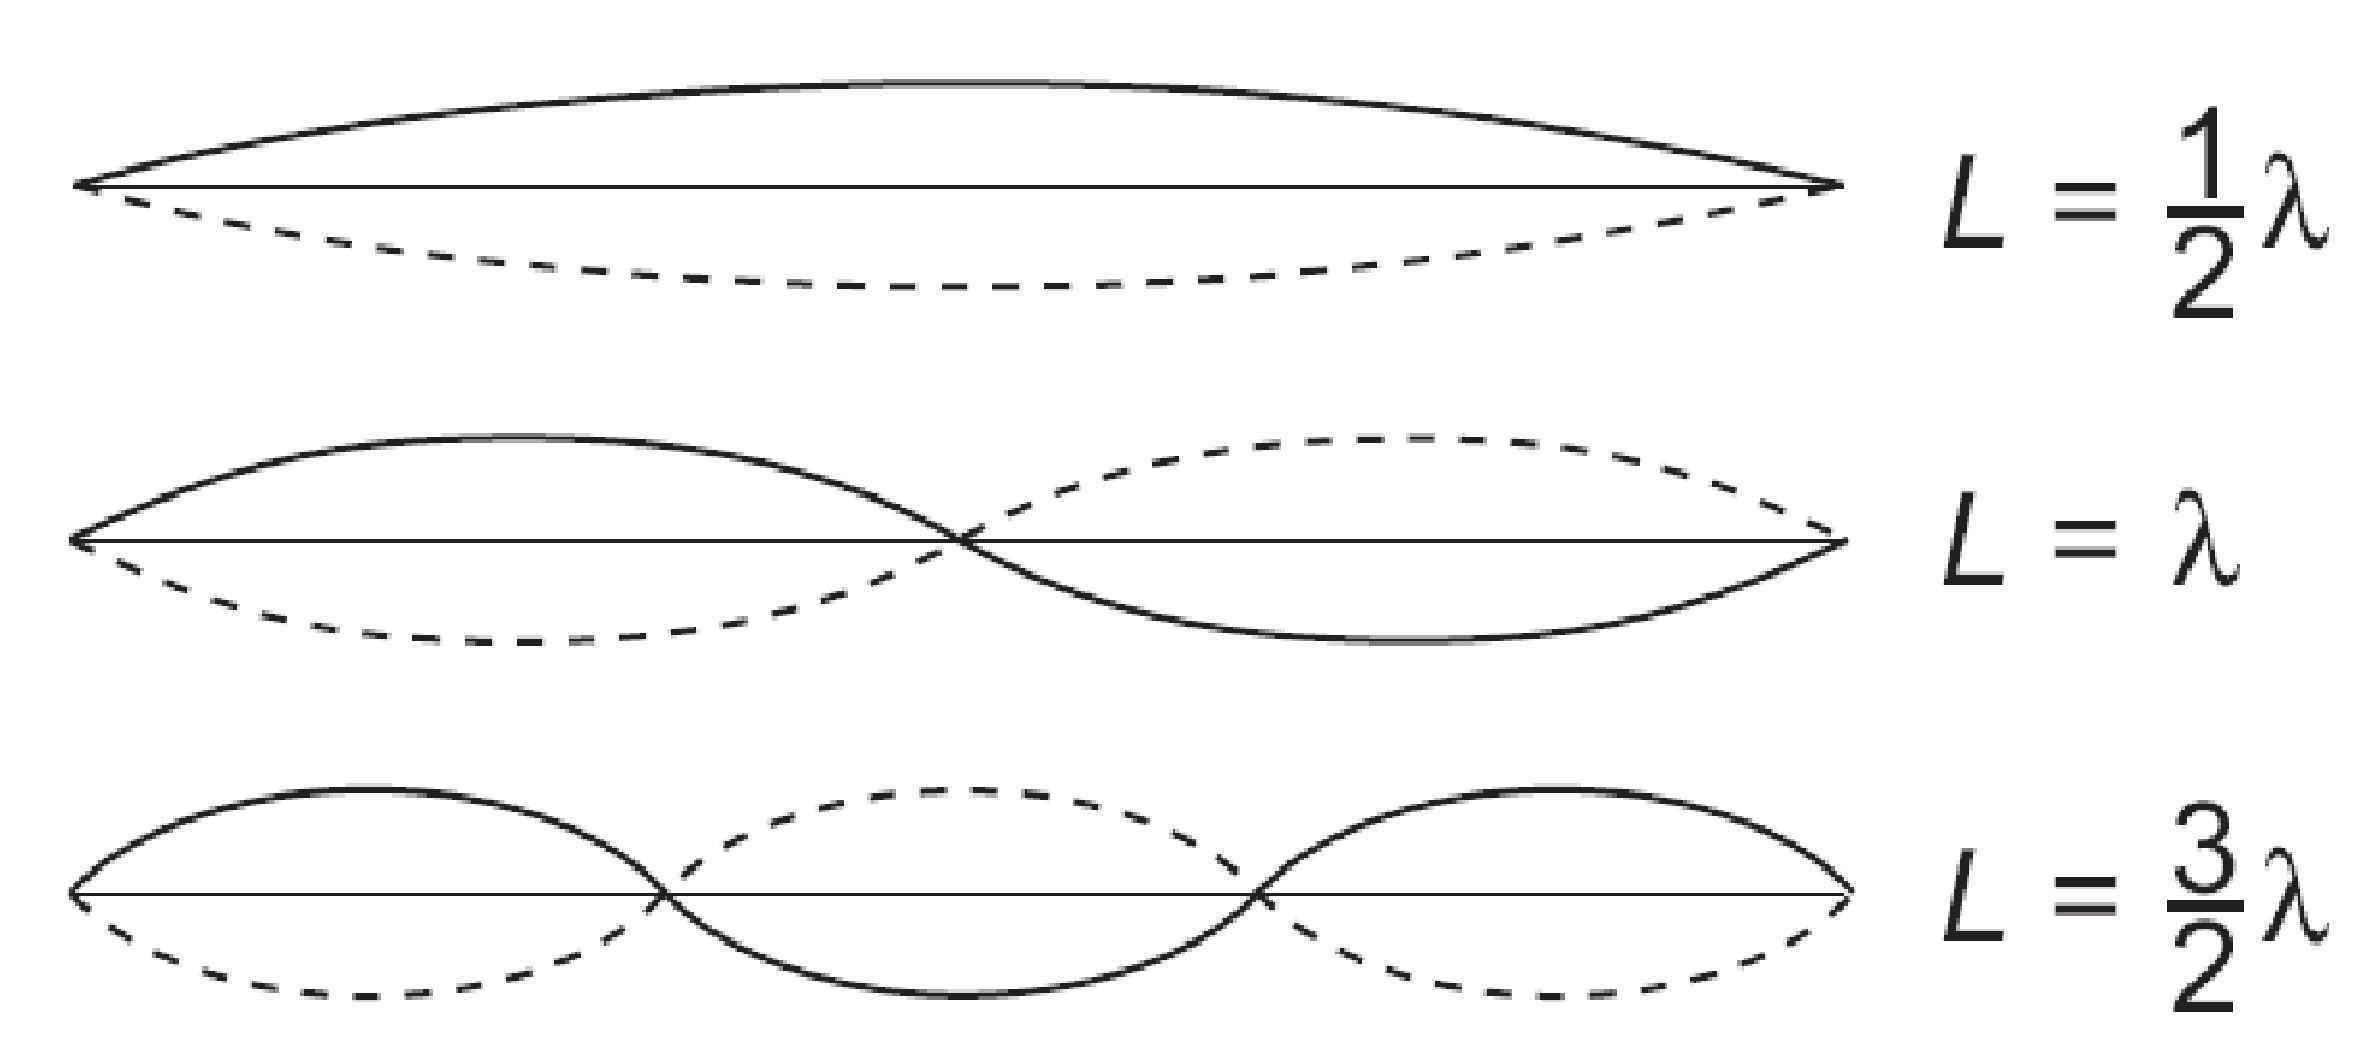
\includegraphics[width=3in]{Standing_waves_strings_fig1_tb.eps}
\end{center}
\vspace{0.3cm}

If you drive a stretched string at an arbitrary frequency, you will probably not see any particular mode; many modes will be mixed together. But, if the tension and the string's length are correctly adjusted to the frequency of the driving vibrator, one vibrational mode will occur at a much greater amplitude than the other modes.
For any wave with wavelength ($\lambda $) and frequency $f$, the speed, $v$, is:
\begin{equation}
v=\lambda f
\end{equation}

The speed of a wave on a string is also given by:
\begin{equation}
v=\sqrt{\frac {T}{\mu }}
\end{equation}
where $T$ is the tension in the string and $\mu $ is the linear density (mass/length) of the string.

In this experiment, standing waves are set up in a stretched string by the vibrations of an electrically-driven String Vibrator. The tension in the string equals the weight of the masses suspended over the pulley. You can alter the tension by
changing the masses. $L$ is the length of the string and $n$ is the number of segments. (Note that $n$ is not the number of nodes). Since a segment is 1/2 wavelength then


\begin{equation}
\lambda =\frac {2L}{n } \qquad n=1,2,3,...
\end{equation}



\vspace{0.3cm}
\begin{center}
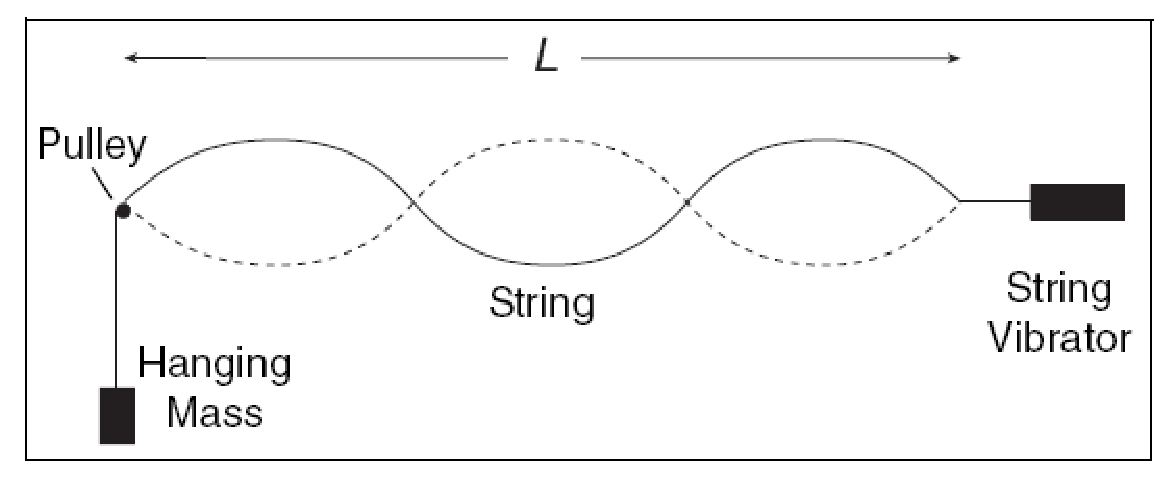
\includegraphics[width=250pt]{Standing_waves_strings_figure2.eps}
\end{center}
\vspace{0.3cm}


\textbf{Procedure}

\textbf{1. } Measure the exact length of a piece of string several meters long. Measure the mass of the
string and calculate the linear density (mass/length).(If your balance is not precise enough to measure that length of string, use a longer
piece of string to calculate the linear density.)

\vspace{2cm}

\textbf{2. } Clamp the String Vibrator and pulley about 100 cm apart. Attach the string to the vibrating blade, run it over the pulley, and hang about 200 g of mass from it. Cut off the excess string.

\textbf{3. } Measure from the knot where the string attaches to the String Vibrator to the top of the pulley.
This is the distance $L$. ($L$ is NOT the total length of the string that you measured in \textbf{1 }.) Record the value here: $L$ =

\vspace{0.3cm}
\begin{center}
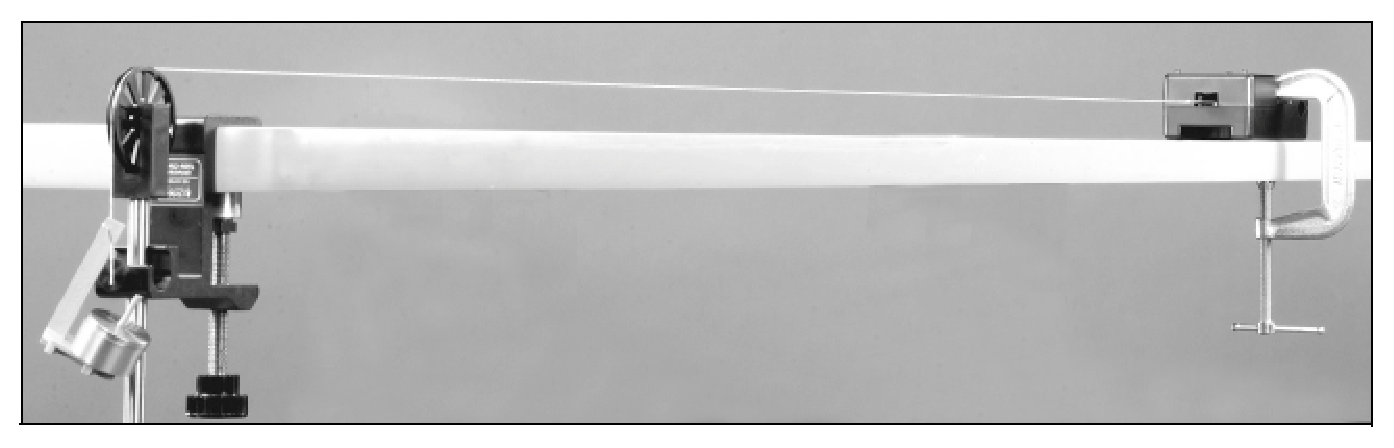
\includegraphics[width=320pt]{Standing_waves_strings_figure3.eps}
\end{center}
\vspace{0.3cm}

\textbf{4. } Connect the AC power supply to the String Vibrator.

\textbf{5. } Adjust the tension by adding to or subtracting from the hanging mass so that the string vibrates in 2 segments. Adjust the tension further to achieve a ``clean'' node at the center. Also check the end of the vibrating blade; the point where the string attaches should be a node. It is more important to have a good node at the blade than it is to have the largest amplitude possible. However, it is desirable to have the largest amplitude possible while keeping a good node.

\textbf{6. } Record the value of the hanging mass $m$ here:

\vspace{3cm}

\textbf{Part A: Speed of the Wave }

\textbf{a. } Calculate the tension in the string. (The weight of the hanging mass provides the tension in the string.)

\vspace{3cm}

\newpage

\textbf{b. } Calculate the speed $v_A$ of the wave from your observed values of tension ($T$) and linear density ($\mu $). Record your calculated value with the correct number of significant figures.


\vspace{4cm}

\textbf{c. } Calculate the speed $v_B$ from the wavelength ($\lambda $) and frequency ($f$). (In the U.S. $f$ = 60.0 Hz.)

\vspace{4cm}

\textbf{d. } Compare the two values ($v_A$ and $v_B$) of speed. What is the difference?

\vspace{4cm}

\textbf{e. } Calculate the percentage by which $v_A$ deviates from $v_B$.

\begin{equation}
\% Deviation =\frac {v_A - v_B}{v_B} \times 100\%
\end{equation}

\vspace{3cm}

\newpage

\textbf{Part B: Linear Density}

\textbf{a. } Produce standing waves of 3, 4, 5, etc. segments in the string. Get as many as you can. Record the mass, $m$, and the number of segments, $n$, in a table here. Be sure to include the results from Part A ($n$ = 2) in the table.

\vspace{6cm}

\textbf{b. } For every value of mass, calculate the tension in the string, and include in the above table.

\textbf{c. } In $Excel$, plot a graph of $T$ versus $n$ and include with this unit. Add a trendline with equation using a power function. What is the power of $n$?
\vspace{20mm}

\textbf{d. } For every value of $n$, calculate $\frac{1}{n^2}$ and include in above table. In $Excel$, plot a graph of $T$ versus $\frac{1}{n^2}$. Does the graph look linear? If so, include a linear trendline with equation. Print the graph and include with this unit.
\vspace{20mm}

\textbf{e. } Record the slope of the graph (including units) here:

\vspace{20mm}

\textbf{f. } Combine the equations in the \textbf{Background } section, and show that the tension can be written as:

\begin{equation}
T=4\mu f^{2}L^{2}\frac{1}{n^2}
\end{equation}

\vspace{25mm}

Thus the slope of a $T$ versus $\frac{1}{n^2}$ graph is $4\mu f^{2}L^{2}$.

\textbf{g. } Use the slope from your graph to calculate the density, $\mu $, of the string. Show that the units are kg/m.

\vspace{5cm}

\textbf{h. } Compare this measured value of string density to the accepted value. (You calculated the accepted value of $\mu $ from the mass and length of the string at the beginning of the experiment). Calculate a percent difference between the two values.

\vspace{50mm}

%\textbf{i. } Calculate the percent deviation of the measured value of $\mu $ from the accepted value.

%\begin{equation}
%\% Deviation =\frac{Measured-Accepted}{Accepted}\times 100\%
%\end{equation}

%\vspace{4cm}

\textbf{Further Investigation}

%\textbf{1. } Hang a mass on the string with a value that is about halfway between the masses that produced standing waves of 3 and 4 segments. The string should show no particular mode. Place a ``bridge'' so that you can see the exact fundamental ($n = 1$) between the String
%Vibrator and the bridge. What is the wavelength?

%\vspace{1.5cm}

%Slide the bridge away from String Vibrator until the string vibrates in 2 segments. How does the wavelength of the two-segment wave compare to the wavelength of the previous one segment wave?

%\vspace{1.5cm}

%Why is a standing wave created only when the bridge is at certain locations? What are these locations called?

%\vspace{1.5cm}

If a strobe is available, observe the standing wave on a string with the 
strobe light. Draw a diagram explaining the motion of the string.




 %lots of uncertainty calculation here.  Might not use this one.
%
\section{Resonance in Tubes}

Name \rule{2.0in}{0.1pt}\hfill{}Section \rule{1.0in}{0.1pt}\hfill{}Date \rule{1.0in}{0.1pt}



{\noindent \bf Objectives:} \begin{list}{$\bullet$}{\itemsep0pt \parsep0pt}

\item Determine the resonant frequency for a tube open at one end.

\item Determine tube lengths at resonance for a tube of variable length.

\item Determine the velocity of sound in air in the laboratory (two ways).

\end{list}

\noindent {\bf Introduction} 

The Economy Resonance Tube is designed for the study of resonance in columns of air.  The tube set includes a movable inner tube with a closed end and an outer tube which is open at both ends.  The inner tube also includes a measuring tape to easily find the length of the air column in the outer tube. To adjust the length of the outer tube, simply slide the inner tube until the desired length appears on the measuring tape.  Open tube experiments can also be performed with the outer tube by removing the inner tube.

\noindent In order that the tube resonate, the frequency of the vibrating air must coincide with the natural frequency of the tube (which may be its fundamental or one of its overtones). For the Economy Resonance Tube, which is closed at one end, this requirement is met if the tube length is an odd number of quarter wavelengths of the sound waves produced by the source ($L = \lambda/4, 3 \lambda/4, 5 \lambda/4$, etc., where $L$ is the length of the tube and $\lambda$ is the wave length of the sound). Note that if the length of the tube is gradually increased while the source is vibrating, the distance between successive resonance positions is $\lambda/2$. \\

\noindent {\small {\bf Note:} Due to edge effects at the open end of a tube, the effective length of the tube depends on the radius of the opening. Thus, $L_{eff} = L + 0.6r$, where $L_{eff}$ is the \textit{effective} length, $L$ is the length measured, and $r$ is the tube radius.} \\


{\noindent \bf Apparatus:} \begin{list}{$\bullet$}{\itemsep0pt \parsep0pt}

\item Economy Resonance Tube 
\item Open speaker
\item Sine wave generator
\item 2 banana plug leads
\item Sound sensor
\item Meter stick
\item Data Studio 750 Interface
\item Thermometer

\end{list}

\noindent Room Temperature ($^\circ$C) \hrulefill \ \  Tube radius (m) \hrulefill

\vspace{5mm}

{\noindent \bf Activity 1: Fixed tube length} \begin{enumerate}

\item Connect the open speaker to the sine wave generator using standard banana plug leads.

\item Adjust the length of the outer tube to 50 cm (check with meter stick).

\item Place the tube in front of the speaker in such a way that the tube is open at one end (the speaker can be set at an angle relative to the tube length).

\item Set the sound sensor inside the tube and connect it to the Data Studio interface.

\item To activate the sound sensor, perform the following sequence:  Start up \textit{DataStudio} by going to \textit{Start} $\rightarrow$ \textit{Programs} $\rightarrow$ \textit{Physics Applications} $\rightarrow$ \textit{DataStudio}.
Click on \textit{Create Experiment}, then \textit{Setup}, then \textit{Add Sensor or Instrument}. Scroll down to \textit{Sound level sensor} and select, then click \textit{OK}. Double click \textit{Graph} at left. Click \textit{Start} to begin taking data.

\item Start at a frequency of 130 Hz and increase until you find the frequency of the largest resonance (indicated by a peak on the sound level graph).  This is the fundamental frequency.  Record the result here:\vspace{10mm}

\item The resonant frequencies for a tube open at one end are given by $f=nv/4L$ where $n$ is an odd integer, $v$ is the velocity of sound and $L$ is the effective tube length.  From the fundamental frequency you just found, calculate the velocity of sound in air (using $n$ = 1) and record it here:\vspace{15mm}

\end{enumerate}

%\noindent {\Large{\bf DATA}} \\

%\noindent Room Temperature ($^\circ$C) \hrulefill \ \  Tube radius (m) \hrulefill

%\begin{center} \begin{tabular}{||c|c|c|c|c|c|c|c|c|c|c|c|c|c|c||} \hline \hline Tuning Fork & \multicolumn{4}{|c|}{First Position of} & \multicolumn{4}{|c|}{Second Position} & \multicolumn{4}{|c|}{Third Position of} & Wave- & Velocity of \\ Frequency, & \multicolumn{4}{|c|}{Resonance, m} & \multicolumn{4}{|c|}{of Resonance, m} & \multicolumn{4}{|c|}{Resonance, m} & length, & Sound in \\ \cline{2-13} Hz & 1 & 2 & 3 & Ave. & 1 & 2 & 3 & Ave. & 1 & 2 & 3 & Ave. & m & air, m/s \\ \hline \hline &&&&&&&&&&&&&& \\ \hline &&&&&&&&&&&&&& \\ \hline \hline \end{tabular} \end{center}


{\noindent \bf Activity 2: Fixed frequency} \begin{enumerate}

\item Adjust the outer tube length to 20 cm.

\item Set the speaker inside the open end of the tube so that it is closed at both ends.

\item Set the sine wave generator frequency to 600 Hz (with low amplitude).

\item Slowly move the inner tube to increase the effective length of the tube.  Record the length of the tube when resonance is achieved. You don't need to use the sound sensor for this. Just listen for maximum loudness.\vspace{10mm}

\item Increase the length of the tube until two more resonance lengths are found for the constant frequency and record them here:\vspace{15mm}

%\item Average your two values to determine your experimental velocity of sound in m/s: \ \ \  \rule{2cm}{1pt}

\item The maxima you have determined are spaced a distance $\lambda/2$ apart, where $\lambda$ is the wavelength.  Find the differences between adjacent resonance lengths and calculate the average of the two values:\vspace{15mm}

\item Find $\lambda$ from your average value of $\lambda/2$ and calculate the velocity of sound in air from $v=f\lambda$.\vspace{15mm}

\item The velocity of sound in air at $0^\circ$C is 331.4 m/s.  The temperature dependence of sound velocity in air is given by $v(T) = 331.4 + 0.6T$, where $T$ is in $^\circ$C and $v$ is in m/s. Calculate an ``accepted'' value of the velocity of sound in air from this formula.

\vspace{15mm}

\item What is the percent difference between your experimental result and the ``accepted'' value?

\end{enumerate}
 

%--------------------------------------------
\part{Thermodynamics}


\section{Heat, Temperature, and Internal Energy}

Name \rule{2.0in}{0.1pt}\hfill{}Section \rule{1.0in}{0.1pt}\hfill{}Date
\rule{1.0in}{0.1pt}

\textbf{Objective}

To investigate the relationship between heat and temperature.

\textbf{Apparatus}

\begin{itemize}
\item Glass beaker 
\item Glass stirring rod
\item Hot plate
\item Ice
\item Data Studio software and temperature probe
\item Clamp and stand
\end{itemize}
\textbf{Temperature of a Substance as a Function of Heat Transfer}

As part of our quest to understand heat energy transfer, temperature,
and internal energy of a substance, let's consider the temperature
change as ice is changed to water and then to steam.

\textbf{Activity 1: Predicting T vs. t for Water} 

Suppose you were to add heat at a constant rate to a container of
ice water at 0\( ^{\circ } \)C until the water begins to boil. Sketch
the predicted shape of the heating curve on the graph below using
a dashed line. Mark the points at which the ice has melted and the
water begins to boil.

\vspace{0.3cm}
{\centering 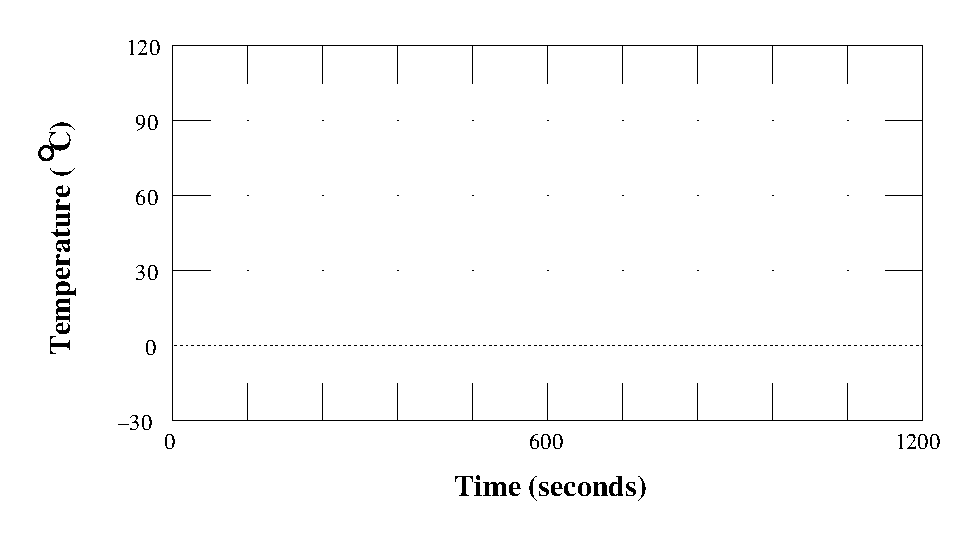
\includegraphics{heat_temp_int_energy_fig_1.eps} \par}
\vspace{0.3cm}

\newpage

\textbf{Activity 2: Measuring T vs. t for Water} 

(a) To test your prediction: 

\begin{enumerate}
\item Fill the glass beaker one third full of ice and set it on top of the hot plate.
\item Suspend the temperature probe so that the end is submerged in the ice but not touching the side or bottom of the beaker. You will need to use the clamp and stand to do this. BE SURE THE WIRE FROM THE TEMPERATURE PROBE IS NOT TOUCHING THE HOT PLATE OR GLASS BEAKER. Also, be sure the temperature probe is attached to port ``A'' of the Pasco interface. Let set for 60 seconds so temperature probe can come to equilibrium with the ice.
\item Open the \textit{Heat, Temp, \& Internal Energy} application in the
132 Workshop folder under \textit{Physics Applications}.
\item Turn on the hot plate to about 6 and click the
\textbf{Start} button on the monitor to begin recording data. The temperature of the water will be recorded on the graph shown on the monitor. Stir often to keep ice against the temperature probe.
\item When ice begins to turn to water, stir at about 1 minute intervals. When all ice is melted, there is no need to stir any further.
\item After the water begins to boil, keep hot plate on for a ninute or two as temperature flattens at 100 degrees.
\item Stop data collection using the \textbf{Stop} button and turn off hot plate.
\item Sketch the shape of the measured heating curve on the above graph
using a solid line. Ignore small variations due to noise and uneven
heating. Mark the points at which the ice has melted and the water
begins to boil.
\end{enumerate}
(b) Does your prediction agree with the measured heating curve? If
not, what are the differences?
\vspace{15mm}

(c) What is the relationship between the temperature and the added
heat while the ice is melting?
\vspace{15mm}

(d) What is the relationship between the temperature and the added
heat after the ice has melted, but before the water begins to boil?
\vspace{15mm}

(e) What is the relationship between the temperature and the added
heat while the water is boiling?
\vspace{15mm}

(f) If there are regions of the heating curve in which the temperature
is not changing, what do you think is happening to the added heat
in these regions?\vspace{15mm}

 %132 equivalent
%\setcounter{equation}{0}
\setcounter{figure}{0}

\section{Calorimetry}

Name \rule{2.0in}{0.1pt}\hfill{}Section \rule{1.0in}{0.1pt}\hfill{}Date
\rule{1.0in}{0.1pt}

\textbf{Purpose}

\begin{itemize}

\item To learn to use a method for measuring heat called calorimetry.

\item To use calorimetry to determine the specific heat of aluminum.

\end{itemize}

\textbf{Apparatus}

\begin{itemize}
\item Hypsometer
\item Hot plate 
\item Aluminum pellets
\item Plastic Beaker
\item Ice 
\item Compact scale (for measuring masses)
\item Calorimeter
\item Temperature probe
\item Glass stirring rod
\item Clamp and stand
\item Safety goggles
\item \textit{DataStudio} software (Calorimetry)
\end{itemize}
\textbf{Introduction} 

Calorimetry is a method for measuring heat. As applied in this experiment,
the method involves the mixing together of substances initially at
two different temperatures. The substances at the higher temperature
lose heat and the substances at the lower temperature gain heat until
thermal equilibrium is reached.

\textbf{Activity 1: Statement of Conservation of Energy}

If no heat is transferred to the surroundings, what is the relationship
between the heat lost by the substances initially at high temperature
and the heat gained by the substances initially at low temperature?
Note: This is simply a statement of conservation of energy.

\vspace{0.3cm}
{\centering \resizebox*{!}{3.5in}{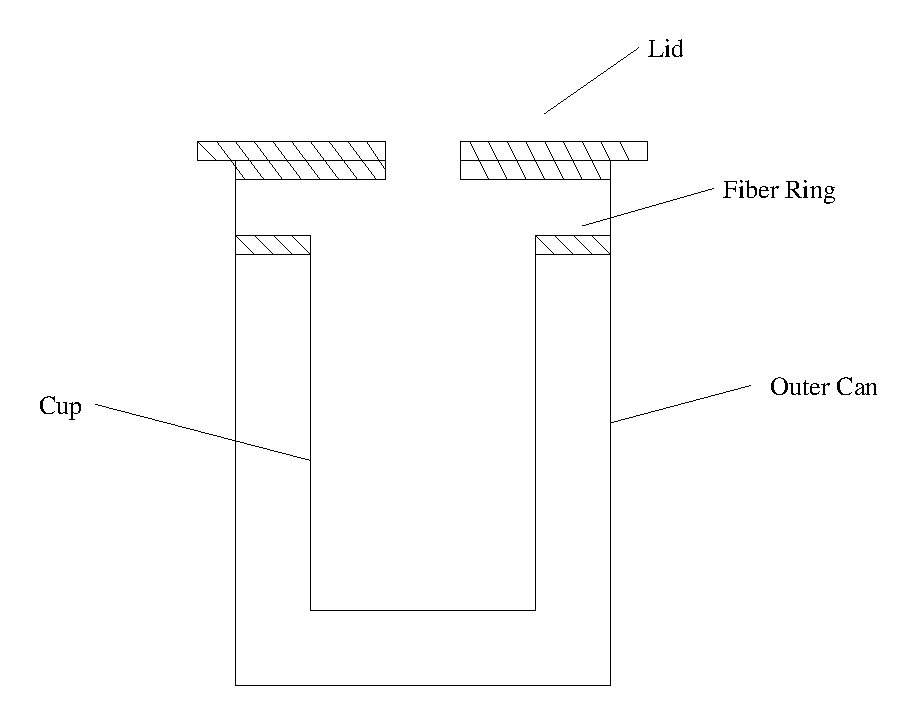
\includegraphics{calorimetry_fig_1.eps}}  \par}
\vspace{0.3cm}

\textbf{Experimental Equipment} 

A calorimeter, shown in the above figure, is used in this experiment
to minimize the exchange of heat between the system and the surroundings.
The inner calorimeter cup is thermally insulated from the surroundings
by suspending it on a ring of material with low heat conductivity
and surrounding it with a layer of air. Also the cup is shiny to minimize
radiation loss. Hence, if the mixture of substances is placed inside
the calorimeter cup, the heat lost to or gained from the surroundings
can be ignored, and the above relationship can be used. The only part
of the calorimeter which is involved in the calculation is the inner
calorimeter cup which contains water and in which an exchange of heat
between the hot and cold bodies takes place. The cup will undergo
the same temperature change as the contained water. Of course, an
instrument will have to be introduced to measure the temperature of
the system, but the heat gained or lost by the instrument is small
and can be ignored.

\textbf{Activity 2: Specific Heat of Aluminum}

(a) Fill the hypsometer (boiler) at least half full of water and start
heating the water.

(b) Determine and record the mass of the hypsometer cup, m\( _{h} \).
Then fill it about half full with dry aluminum pellets. Determine
and record the mass of the cup and pellets, m\( _{hp} \), and calculate
the mass of the pellets, m\( _{p} \). Record the measurements in
the space below.
\vspace{15mm}

(c) Fill the plastic beaker with ice water. Open the \textit{Calorimetry.ss}
application in the 132 Workshop folder in the {\bf Start} menu and start
collecting data. To make sure the temperature probe is working 
properly place it in the ice water and
check that it is reading approximately 0\( ^{\circ } \)C. If not,
then consult your instructor.

(d) Place the hypsometer cup in the top of the hypsometer and put the temperature probe into the middle of the pellets.  To do this, remove the pellets from the cup, place the temperature probe in the proper position (using the clamp and stand), then return the pellets to the cup.

(e) Determine and record the mass of the calorimeter cup, m\( _{c} \).
Fill this cup about half full of cold tap water. Determine and record
the mass of the cup and water, m\( _{cw} \), and calculate the mass
of the water, m\( _{w} \). Then place the calorimeter cup in the outer
can and put the lid on.
\vspace{15mm}

(f) When the temperature of the pellets becomes constant, at or near
100\( ^{\circ } \)C, record the temperature of the pellets as T\( _{p} \).
Remove the probe from the pellets and put it in the cold water in the calorimeter cup. When the temperature of the water levels off, record it as T\( _{w} \).
\vspace{15mm}

(g) Now, quickly but carefully, pour the pellets into the water in
the calorimeter cup. Stir the water occasionally with the stirring rod and
monitor the temperature of the mixture. When the temperature levels off, record
this value as T. Click the {\bf Stop} button on the monitor, print your graph 
of temperature as a function of time and include it in this unit.
\vspace{15mm}

(h) Write the complete heat equation and solve for the unknown specific
heat of the metal. 
The specific heat of the calorimeter cup is 900 J/kg-\( ^{\circ } \)C.
\vspace{2in}

(i) Look up the accepted value for the specific heat of aluminum and
calculate the percent difference between this value and the one you
determined above. Do the two values agree within experimental uncertainties?
Comment on possible sources of error.
\vspace{25mm}

%\textbf{Activity 3: Specific Heat of Metals}

%(a) Repeat steps 2(a)-2(i) with pellets of a different metal besides aluminum.
%Record the the type of metal, the mass of the pellets, the temperature of the
%pellets just before you pour them in the cold water, and the temperature of the
%combined pellets, water, and cup.
%\vspace{15mm}

%\newpage 

%(b) Use the equation you derived above for the unknown specific
%heat of the new metal. 
%The specific heat of the calorimeter cup is 900 J/kg-\( ^{\circ } \)C.

%\vspace{2.5cm}

%(c) Look up the accepted value for the specific heat of your new metal and
%calculate the percent difference between this value and the one you
%determined above. 
%\vspace{20mm}

\textbf{Activity 3: Average and Standard Deviation}

Consult the other lab groups in class and record their values of the specific
heat of aluminum below. Calculate the average and standard deviation.
\vspace{2in}


%\textbf{Activity 4: Heat of Fusion of Ice}

%(a) The heat of fusion of ice is found experimentally as follows:
%A known mass of warm water is placed in the calorimeter cup and its
%temperature recorded. A known mass of ice at 0\( ^{\circ } \)C (with
%no water) is added to the water and allowed to melt. The final temperature
%of the mixture after the ice has melted is recorded. Perform the experiment
%and record the data in the space below.

%\vspace{25mm}

%(b) Write the complete heat equation and solve for the unknown heat
%of fusion of ice.\vspace{25mm}

  %132 equivalent

\section{Boyle's Law}

Name \rule{2.0in}{0.1pt}\hfill{}Section \rule{1.0in}{0.1pt}\hfill{}Date
\rule{1.0in}{0.1pt}

\textbf{Objective}

To investigate the relationship between the pressure and volume of
a gas.

\textbf{Apparatus}

\begin{itemize}
\item DataStudio 750 Interface
\item Pasco Pressure Sensor
\item Syringe
\item Tubing
\end{itemize}
\vspace{0.3cm}
{\par\centering 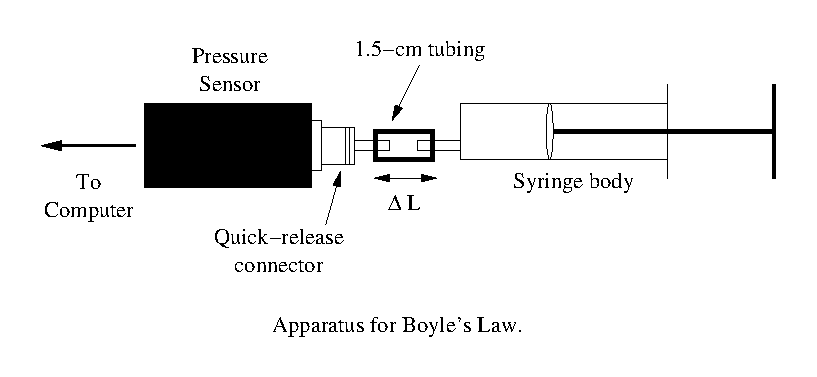
\includegraphics{boyleslawfig1.eps} \par}
\vspace{0.3cm}

\textbf{Introduction}

The behavior of a gas can be described in terms of the macroscopic quantities:
temperature (T), pressure (P), and volume (V). The relationship between these
quantities is given by the equation of state of the gas. A real gas behaves
approximately as an ideal gas if it is far from liquefaction. In that case,
the equation of state of an ideal gas can be used to describe a real gas. For
a given mass of a gas, if one of the quantities P, T, or V is changed, a change
in the other two quantities probably will result. However, if one of the quantities
is kept constant, the relationship between the other two can be studied. The
relationship between pressure and volume of an ideal gas is called Boyle's law.

The experimental apparatus is shown in the figure above. The gas is air contained
in a syringe that has marking on its side to measure the volume of the syringe.
A short tube connects the syringe with a pressure sensor that measures the pressure
in the tube and converts that measurement into a signal that can be read by
the DataStudio interface.

\textbf{Activity 1: Relationship Between P and V of a Gas}

(a) Check that there are no leaks in the apparatus by trying to compressing
the syringe from the 20.0 ml position to the 10.0 ml position. It should become
increasingly difficult to push the plunger as the volume decreases. If this
is not the case, check the couplings for fit. If no problem is obvious, then
consult your instructor. 
\vspace{20mm}

(b) The initial volume of air in the syringe should be set at 20.0 ml. If your
syringe is set to some other value, disconnect the quick release connector from
the sensor by gently rotating it in the counter-clockwise direction as you look
from the syringe toward the pressure sensor. Next, move the piston to the 20.0
ml position, and then re-connect the quick release connector to the pressure
sensor. 

(c) \textbf{Data Recording}. Open the Boyle's Law activity located in the 132
Workshop Folder under the {\bf Start} menu. Click on the window labeled \textit{Volume
and Pressure Table}. This is where your data will be displayed as you record
it. This table display will show the values of the gas volume in the syringe
which you will set by moving the piston to the appropriate marking on the syringe.
You will record the pressure at each of these settings with the pressure sensor.
To begin recording data, make sure the piston is at the 20-ml setting, and click
the Start button. The Start button will change to a Keep button and the table
display will show the value of the pressure next to the first volume value (20
ml) in the table. The reading in the pressure column should be colored red.
Click the Keep button to record this pressure (notice the reading in the Pressure
column beside the 20-ml entry changes from red to black). The next setting for
the volume (18 ml) will appear in the Volume column of the data table display.

NOTE: For the first pressure reading at 20 ml, the air in the syringe will be
in thermal equilibrium with the environment. This will not be the case immediately
after compressing the syringe for the next reading. Therefore, you must allow
one second for the system to return to thermal equilibrium after you compress
the syringe and before clicking on Keep to record pressure values. 

(d) Compress the syringe to the next value of the volume as listed in the data
display table (i.e., the window labeled \textit{Volume and Pressure Table})
and wait one second for the system to reach thermal equilibrium. Once thermal
equilibrium is reached, click Keep to record the pressure. The data table display
will automatically change to show the next value of the volume at which the
pressure will be measured. 

(e) Repeat step (d) for the remaining values of the volume listed in the table
display. In other words, continue taking pressure measurements at the prescribed
volume values in the data table display by moving the piston to the prescribed
value and clicking on Keep after thermal equilibrium is reached. After you record
the pressure for the last volume (8 ml), click the small, red box next to the
Keep button (this is the stop button) to end data recording.

(f) \textbf{Analysis.} What happened to the pressure when the volume was 
reduced from 20 ml to 8 ml?  From looking at the data, do the pressure and 
volume seem to be directly or inversely proportional? Explain. 
\vspace{25mm}

(g) Copy your data into a spreadsheet and plot pressure versus volume. Next, 
fit your data with a trendline using a power function. Record the result here.
What should you get for the power of $V$? Why?
\vspace{25mm}

(h) If pressure and volume are inversely proportional, then what can you say
about the product of pressure and volume? Explain.
\vspace{35mm}

\newpage

(i) The measurements you have made are V in milliliters (ml) and P in 
kilopascals (kPa). What are the corresponding units of PV? Show how you get 
this here (the result must be in energy units).
\vspace{50mm}

(j) Construct a table in the space below with the column headings: V (ml), P
(kPa), and PV. Include the units from above in the last column.  Enter the 
results for P and V in this new table and calculate
PV for each set of readings. Determine the mean value and the standard deviation
\( \sigma  \) for PV. Record the results in the form PV = Mean \( \pm \, \sigma  \)
. What does this result tell you about the product PV? What does it tell you
about the relationship between P and V? Explain.
\vspace{75mm}

(k) Is there a trend in the values of PV as the volume decreases? If so, what 
do you suppose causes this trend?

%(l) Examine the plot below with results from two different data runs. How do
%you explain the difference between the curves for the different tubing lengths
%(\( \triangle L \) in the diagram on page 11)?

%\vspace{0.3cm}
%{\par\centering 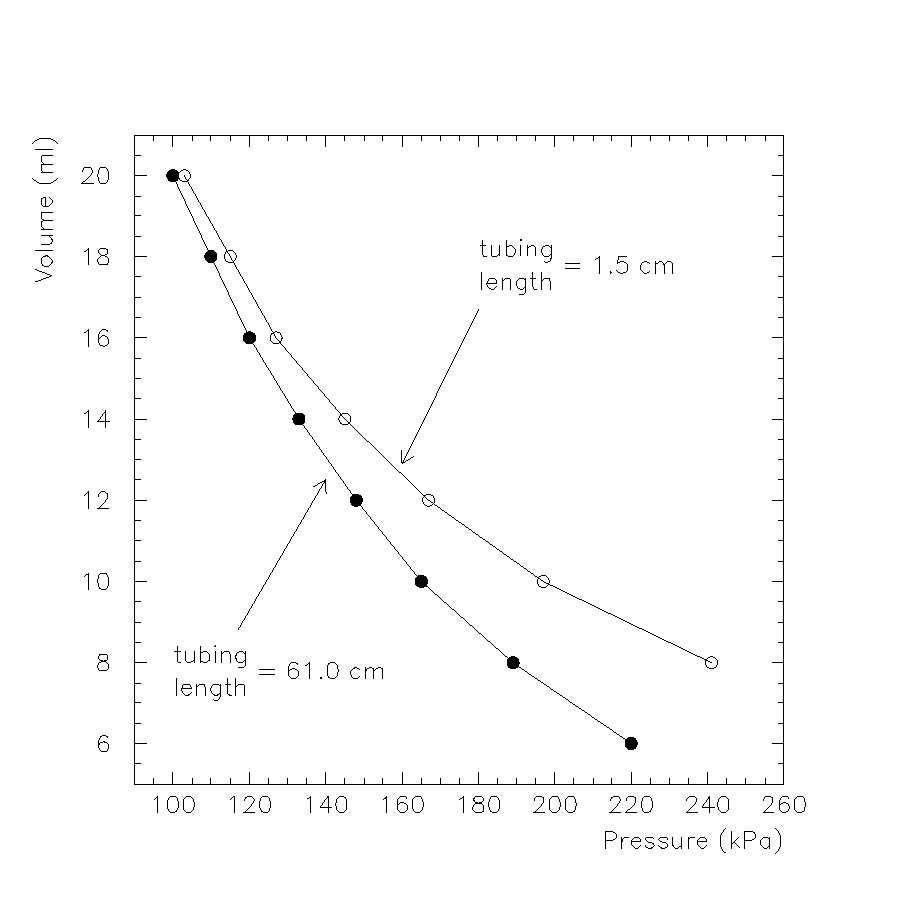
\includegraphics{boyleslawfig2.eps} \par}
%\vspace{0.3cm}

%{\par\centering Results of measurement with Boyle's Law apparatus \par}

%{\par\centering different values of \( \triangle L \), the tubing length.\par}

 %132 equivalent
\setcounter{equation}{0}
\setcounter{figure}{0}

\section{Calorimetry}

Name \rule{2.0in}{0.1pt}\hfill{}Section \rule{1.0in}{0.1pt}\hfill{}Date
\rule{1.0in}{0.1pt}

\textbf{Purpose}

\begin{itemize}

\item To learn to use a method for measuring heat called calorimetry.

\item To use calorimetry to determine the specific heat of aluminum.

\end{itemize}

\textbf{Apparatus}

\begin{itemize}
\item Hypsometer
\item Hot plate 
\item Aluminum pellets
\item Plastic Beaker
\item Ice 
\item Compact scale (for measuring masses)
\item Calorimeter
\item Temperature probe
\item Glass stirring rod
\item Clamp and stand
\item Safety goggles
\item \textit{DataStudio} software (Calorimetry)
\end{itemize}
\textbf{Introduction} 

Calorimetry is a method for measuring heat. As applied in this experiment,
the method involves the mixing together of substances initially at
two different temperatures. The substances at the higher temperature
lose heat and the substances at the lower temperature gain heat until
thermal equilibrium is reached.

\textbf{Activity 1: Statement of Conservation of Energy}

If no heat is transferred to the surroundings, what is the relationship
between the heat lost by the substances initially at high temperature
and the heat gained by the substances initially at low temperature?
Note: This is simply a statement of conservation of energy.

\vspace{0.3cm}
{\centering \resizebox*{!}{3.5in}{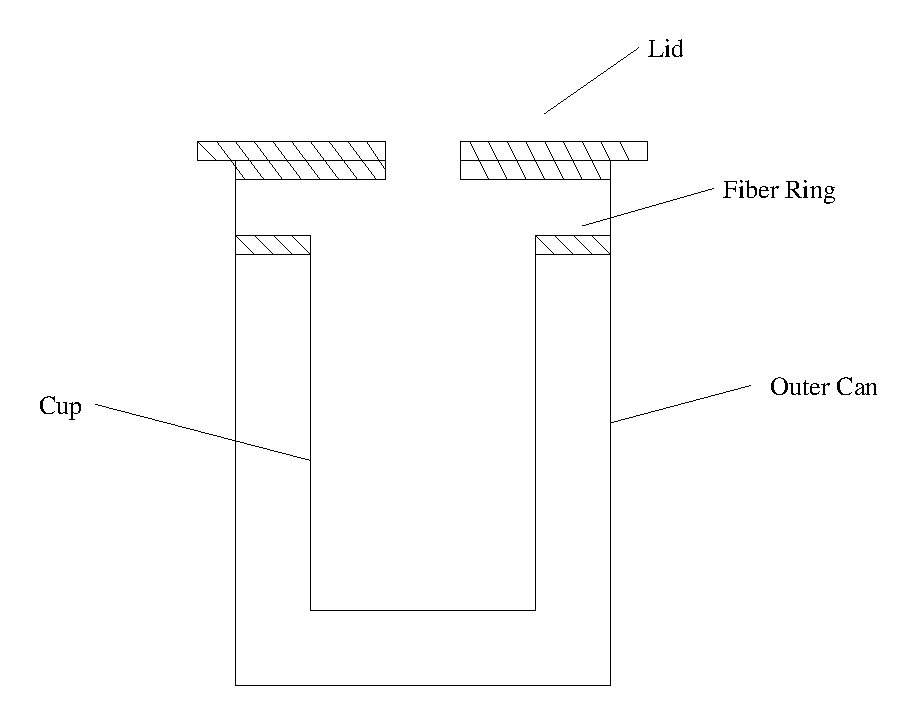
\includegraphics{calorimetry_fig_1.eps}}  \par}
\vspace{0.3cm}

\textbf{Experimental Equipment} 

A calorimeter, shown in the above figure, is used in this experiment
to minimize the exchange of heat between the system and the surroundings.
The inner calorimeter cup is thermally insulated from the surroundings
by suspending it on a ring of material with low heat conductivity
and surrounding it with a layer of air. Also the cup is shiny to minimize
radiation loss. Hence, if the mixture of substances is placed inside
the calorimeter cup, the heat lost to or gained from the surroundings
can be ignored, and the above relationship can be used. The only part
of the calorimeter which is involved in the calculation is the inner
calorimeter cup which contains water and in which an exchange of heat
between the hot and cold bodies takes place. The cup will undergo
the same temperature change as the contained water. Of course, an
instrument will have to be introduced to measure the temperature of
the system, but the heat gained or lost by the instrument is small
and can be ignored.

\textbf{Activity 2: Specific Heat of Aluminum}

(a) Fill the hypsometer (boiler) at least half full of water and start
heating the water.

(b) Determine and record the mass of the hypsometer cup, m\( _{h} \).
Then fill it about half full with dry aluminum pellets. Determine
and record the mass of the cup and pellets, m\( _{hp} \), and calculate
the mass of the pellets, m\( _{p} \). Record the measurements in
the space below.
\vspace{15mm}

(c) Fill the plastic beaker with ice water. Open the \textit{Calorimetry.ss}
application in the 132 Workshop folder in the {\bf Start} menu and start
collecting data. To make sure the temperature probe is working 
properly place it in the ice water and
check that it is reading approximately 0\( ^{\circ } \)C. If not,
then consult your instructor.

(d) Place the hypsometer cup in the top of the hypsometer and put the temperature probe into the middle of the pellets.  To do this, remove the pellets from the cup, place the temperature probe in the proper position (using the clamp and stand), then return the pellets to the cup.

(e) Determine and record the mass of the calorimeter cup, m\( _{c} \).
Fill this cup about half full of cold tap water. Determine and record
the mass of the cup and water, m\( _{cw} \), and calculate the mass
of the water, m\( _{w} \). Then place the calorimeter cup in the outer
can and put the lid on.
\vspace{15mm}

(f) When the temperature of the pellets becomes constant, at or near
100\( ^{\circ } \)C, record the temperature of the pellets as T\( _{p} \).
Remove the probe from the pellets and put it in the cold water in the calorimeter cup. When the temperature of the water levels off, record it as T\( _{w} \).
\vspace{15mm}

(g) Now, quickly but carefully, pour the pellets into the water in
the calorimeter cup. Stir the water occasionally with the stirring rod and
monitor the temperature of the mixture. When the temperature levels off, record
this value as T. Click the {\bf Stop} button on the monitor, print your graph 
of temperature as a function of time and include it in this unit.
\vspace{15mm}

(h) Write the complete heat equation and solve for the unknown specific
heat of the metal. 
The specific heat of the calorimeter cup is 900 J/kg-\( ^{\circ } \)C.
\vspace{2in}

(i) Look up the accepted value for the specific heat of aluminum and
calculate the percent difference between this value and the one you
determined above. Do the two values agree within experimental uncertainties?
Comment on possible sources of error.
\vspace{25mm}

%\textbf{Activity 3: Specific Heat of Metals}

%(a) Repeat steps 2(a)-2(i) with pellets of a different metal besides aluminum.
%Record the the type of metal, the mass of the pellets, the temperature of the
%pellets just before you pour them in the cold water, and the temperature of the
%combined pellets, water, and cup.
%\vspace{15mm}

%\newpage 

%(b) Use the equation you derived above for the unknown specific
%heat of the new metal. 
%The specific heat of the calorimeter cup is 900 J/kg-\( ^{\circ } \)C.

%\vspace{2.5cm}

%(c) Look up the accepted value for the specific heat of your new metal and
%calculate the percent difference between this value and the one you
%determined above. 
%\vspace{20mm}

\textbf{Activity 3: Average and Standard Deviation}

Consult the other lab groups in class and record their values of the specific
heat of aluminum below. Calculate the average and standard deviation.
\vspace{2in}


%\textbf{Activity 4: Heat of Fusion of Ice}

%(a) The heat of fusion of ice is found experimentally as follows:
%A known mass of warm water is placed in the calorimeter cup and its
%temperature recorded. A known mass of ice at 0\( ^{\circ } \)C (with
%no water) is added to the water and allowed to melt. The final temperature
%of the mixture after the ice has melted is recorded. Perform the experiment
%and record the data in the space below.

%\vspace{25mm}

%(b) Write the complete heat equation and solve for the unknown heat
%of fusion of ice.\vspace{25mm}

 %132 equivalent
%
\section{Charles' Law}

Name \rule{2.0in}{0.1pt}\hfill{}Section \rule{1.0in}{0.1pt}\hfill{}Date
\rule{1.0in}{0.1pt}+

\textbf{Objectives} 

To investigate the relationship between volume and temperature for
a constant mass of gas at constant pressure and determine the value
of absolute zero.

\textbf{Apparatus} 

\begin{itemize}
\item Charles law apparatus with stand
\item Temperature sensor
\item Air chamber and tubing
\item Hot plate
\item Glass beaker
\item Clamp and stand
\end{itemize}
\vspace{0.3cm}

\begin{figure}[hbt]
\begin{center}
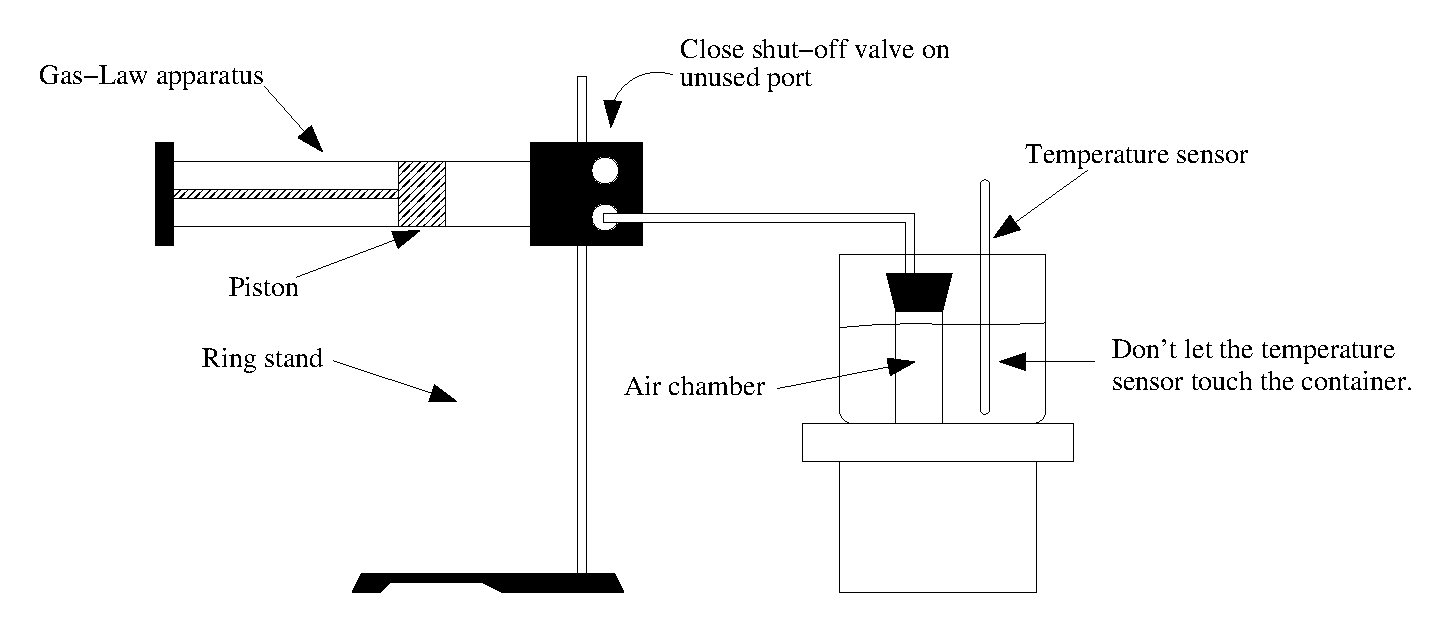
\includegraphics[width=6.0in]{charles_law_fig1.eps}
\caption{Charles' Law apparatus.}
\end{center}
\end{figure}

\textbf{Introduction}

The behavior of a gas can be described in terms of the macroscopic quantities:
temperature (T), pressure (P), and volume (V). The relationship between these
quantities is given by the equation of state of the gas. A real gas behaves
approximately as an ideal gas if it is far from liquefaction. In that case,
the equation of state of an ideal gas can be used to describe a real gas. For
a given mass of a gas, if one of the quantities P, T, or V is changed, a change
in the other two quantities probably will result. However, if one of the quantities
is kept constant, the relationship between the other two can be studied. The
relationship between temperature and volume of an ideal gas is called Charles' law.

The experimental apparatus is shown in the figure above and consists
of an air chamber containing dry air. The pressure on the air in the chamber is due to atmospheric
pressure applied through the movable piston.

\textbf{Activity 1: V-T Relationship for a Gas}

(a) Check that there are no leaks in the apparatus by trying to compressing
the piston from the 100 mm position to the 10 mm position. It should become
increasingly difficult to push the plunger as the volume decreases. If this
is not the case, check the couplings for fit. If no problem is obvious, then
consult your instructor. 

(b) Open the {\it Charles' Law} activity in the 132 Workshop Folder under the
{\bf Start} menu.
Click on the window labeled \textit{Charles' Law Table}. 
This is where your data will be displayed as you record
it. This table display will show the values of the gas temperature in the air chamber
and the entry number.
The data-taking procedure you will follow is described here first.
One member of your team will heat the air chamber in the flask on the hot plate 
and call out the position of the piston.
Another member will record the position settings by hand in the table below
and
click the {\bf Keep} button on the {\it DataStudio} interface to record the 
temperature for that entry.
To begin recording data, make sure the piston is at the low end of the scale, and click
the {\bf Start} button on the {\it DataStudio} interface. 
The {\bf Start} button will change to a {\bf Keep} button and the table
display will show the value of the temperature next to the first entry in the table. 
The reading in the temperature column should be colored red.
Click the {\bf Keep} button to record this temperature (notice the reading in the Temperature
column beside the entry number changes from red to black). The next entry number
 will appear in the Entry column of the data table display.

%NOTE: For the first temperature reading, the air in the chamber will be
%in thermal equilibrium with the environment. This will not be the case immediately
%after adding ice for the next reading. Therefore, you must allow
%3-5 seconds for the system to return to thermal equilibrium after you add ice
% and before clicking on {\bf Keep} to record temperature values. 

(c) Now, immerse the air chamber in a beaker of cold, tap water water and click
{\bf Start} on the {\it DataStudio} interface. You can monitor the temperature
on the temperature versus time plot to the right.
Make sure the set screw on the side of the piston is released.

(d) When the temperature is stable click {\bf Keep} and that point will be recorded in the
table. One team member should read off the piston position while the other 
writes it in the table at the same time.

(e) Now turn up the heat. The piston will move as the gas expands.
Read out the position of the piston every one or two millimeters. The other team member
will click {\bf Keep} (recording the temperature) and record the piston position
in the table.

(f) Repeat step (e) until the piston no longer moves or the water starts to boil.
 
(g) Calculate the volume of the apparatus for each piston position and plot
this volume versus temperature. The diameter of the Gas-Law apparatus is written on its
base.

\vspace{0.3cm}
{\centering \begin{tabular}{|c|c|c|c|}
\hline 
~~~Entry Number~~~&
~~~Piston Position (mm)~~~&
~~~Gas-Law Apparatus Volume (ml)~~~&
~~~Temperature ($^\circ  \rm C$)~~~\\
\hline
\hline 
&
&
&
\\
\hline 
&
&
&
\\
\hline 
&
&
&
\\
\hline 
&
&
&
\\
\hline 
&
&
&
\\
\hline 
&
&
&
\\
\hline 
&
&
&
\\
\hline 
&
&
&
\\
\hline 
&
&
&
\\
\hline
&
&
&
\\
\hline
&
&
&
\\
\hline
&
&
&
\\
\hline
&
&
&
\\
\hline
&
&
&
\\
\hline
\end{tabular}\par}
\vspace{0.3cm}

(h) How are the volume and temperature related?
Fit your data with the appropriate function and record the results here.
Print your plot and attach it to this unit.
\vspace{15mm}

(h) Repeat steps c-h to obtain a second {\it V-T} curve. Record your data in the table below
along with the fit to the V-T data.
\vspace{30mm}


\vspace{0.3cm}
{\centering \begin{tabular}{|c|c|c|c|}
\hline 
~~~Entry Number~~~&
~~~Piston Position (mm)~~~&
~~~Gas-Law Apparatus Volume (ml)~~~&
~~~Temperature ($^\circ  \rm C$)~~~\\
\hline
\hline 
&
&
&
\\
\hline 
&
&
&
\\
\hline 
&
&
&
\\
\hline 
&
&
&
\\
\hline 
&
&
&
\\
\hline 
&
&
&
\\
\hline 
&
&
&
\\
\hline 
&
&
&
\\
\hline 
&
&
&
\\
\hline
&
&
&
\\
\hline
&
&
&
\\
\hline
&
&
&
\\
\hline
&
&
&
\\
\hline
&
&
&
\\
\hline
\end{tabular}\par}
\vspace{2.0cm}

\textbf{Activity 2: Absolute Zero and the Kelvin Scale}

(a) The absolute zero of temperature can be defined as the temperature
at which the volume of an ideal gas is zero. Determine absolute
zero from the equation of your graph by setting V = 0 and solving for T.
\vspace{30mm}

(b) Determine the percent difference between your value of absolute
zero and the accepted value of -273\( ^{\circ } \)C. Are you happy or sad?
\vspace{30mm}

(c) Record the results from the other groups in class.
Obtain an average and standard deviation and record it here.
Are your results consistent with the class average? Explain.

 %132 equivalent
%
\section{The P-T Relationship of a Gas}

Name \rule{2.0in}{0.1pt}\hfill{}Section \rule{1.0in}{0.1pt}\hfill{}Date
\rule{1.0in}{0.1pt}+

\textbf{Objectives} 

To investigate the relationship between pressure and temperature for
a constant mass of gas at constant volume and determine the value
of absolute zero.

\textbf{Apparatus} 

\begin{itemize}
\item Pressure sensor
\item Temperature sensor
\item Air chamber and tubing
\item Hot plate
\item Glass beaker
\item Clamp and stand
\end{itemize}
\vspace{0.3cm}

\begin{figure}[hbt]
\begin{center}
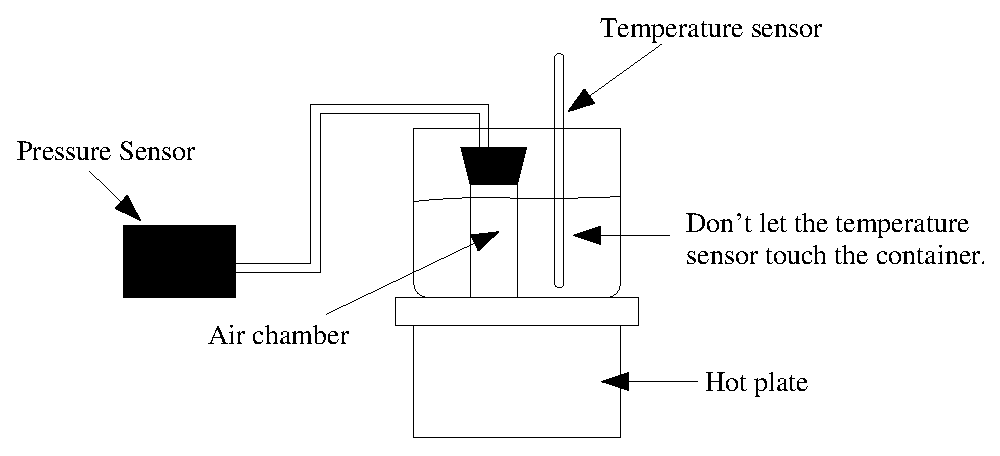
\includegraphics[width=6.0in]{P-T_fig1b.eps}
\caption{P-T apparatus.}
\end{center}
\end{figure}

\textbf{Introduction}

The behavior of a gas can be described in terms of the macroscopic quantities:
temperature (T), pressure (P), and volume (V). The relationship between these
quantities is given by the equation of state of the gas. A real gas behaves
approximately as an ideal gas if it is far from liquefaction. In that case,
the equation of state of an ideal gas can be used to describe a real gas. For
a given mass of a gas, if one of the quantities P, T, or V is changed, a change
in the other two quantities probably will result. However, if one of the quantities
is kept constant, the relationship between the other two can be studied. The
relationship between temperature and pressure of an ideal gas is known as 
Gay-Lussac's law.

The experimental apparatus is shown in the figure above and consists
of an air chamber containing dry air. The volume of the gas is fixed.

\textbf{Activity 1: P-T Relationship for a Gas}

(a) Fill the beaker 3/4 full with cold tap water and place it on the hot plate.  Immerse the air chamber in the water so that most of the volume of the air chamber is submerged.  The air chamber will have to be held in place with a clamp and stand or it will float to the top.  Set the temperature sensor in the water in such a way that it is not touching the side or bottom of the beaker.

(b) Open the {\it P-T} activity in the 132 Workshop Folder under the
{\bf Start} menu.
Click on the window labeled \textit{Temperature and Pressure Table}. 
This is where your data will be displayed as you record
it. This table display will show the values of the gas pressure in the air chamber and
the temperature of the heat bath. 
To begin recording data click
the {\bf Start} button on the {\it DataStudio} interface. 
The {\bf Start} button will change to a {\bf Keep} button and the table
display will show the values of the temperature and pressure. 
Click the {\bf Keep} button to record this temperature and pressure.

(c) Turn the hot plate on high.  As the temperature rises, click the {\bf Keep} button when the temperature is 5-7\( ^{\circ } \) above its first value.  Continue recording the temperature and pressure at 5-7\( ^{\circ } \) intervals (by clicking the {\bf Keep} button) until the water is close to boiling.  You can monitor the temperature on the temperature versus time plot to the right (on the monitor) or by watching the temperature in the \textit{Temperature and Pressure Table}.  After your last reading, click the small red box next to the {\bf Keep} button (this is the stop button) to end data recording.

(d) How are the pressure and temperature related?  Print your data table, enter the data in \textit{Excel} and plot pressure vs temperature on a linear graph, showing the equation of the graph.  Print this graph and add it to this unit. 
Write the equation here as pressure (P) as a function of temperature (T), 
including units on the constants.
\vspace{15mm}



\textbf{Activity 2: Absolute Zero and the Kelvin Scale}

(a) The absolute zero of temperature can be defined as the temperature
at which the pressure of an ideal gas is zero. Determine absolute
zero from the equation of your graph by setting P = 0 and solving for T.
\vspace{30mm}

(b) Record the results from the other groups in class.
Obtain an average and standard deviation and record it here.
Are your results consistent with the class average?  Explain.
\vspace{30mm}

(c) Does there appear to be a systematic error in the class results relative 
to the accepted value of -273\( ^{o } \)C? If so, what do you suppose 
causes the error? Think about this and try to explain.

 %132 equivalent

%--------------------------------------------
\part{Mechanical Waves}

\section{Music to Our Ears: Standing Waves in Strings}

Name \rule{2.0in}{0.1pt}\hfill{}Section \rule{1.0in}{0.1pt}\hfill{}Date
\rule{1.0in}{0.1pt}

\textbf{Aim:}
\begin{itemize}
\item  to study the natural modes of vibration of a stretched string
\end{itemize}

\textbf{Equipment:}
\begin{itemize}
\item  string vibrator and power supply
\item  inelastic braided string
\item  2 clamps
\item  superpulley
\item  mounting rod for the superpulley
\item  mass and hanger set
\item  balance
\item  tape measure
\end{itemize}


How do we make musical sounds? To make a sound , we need something that vibrates. If we want to make musical notes you usually need the vibration to have an almost constant frequency: that means stable pitch. We also want a frequency that can be easily controlled by the player. In electronic instruments this is done with electric circuits or with clocks and memories. In non-electronic instruments, the stable, controlled vibration is produced by a standing wave. Here we discuss the way strings work. This is also a good introduction for studying wind instruments, because vibrating strings are easier to visualise than the vibration of the air in wind instruments, but the math is very similar.  

\textbf{Introduction}

Waves are oscillations in an elastic medium:

\begin{itemize}
\item  your own vocal cords (the medium) vibrating as air is forced over them by your lungs; 
\item  a stretched string (the medium) on a musical instrument vibrating as it is bowed, hammered or plucked; 
\item  pressure oscillations in a column of air (the medium) in a wind instrument, organ pipe or your own oral and nasal cavities.
\end{itemize}

In each case the medium has an equilibrium state, and when displaced or otherwise perturbed from that state, experiences a force which tends to restore it to equilibrium. For small perturbations, the restoring force is proportional to the displacement and the medium becomes a simple harmonic oscillator.

There are also waves that do not require a medium, namely electromagnetic waves, which will be discussed later in the course.

\textbf{Background}

Standing waves (stationary waves) are produced by the interference of two traveling waves, both of which have the
same wavelength, speed and amplitude, but travel in opposite directions through the same medium. The necessary conditions for the production of
standing waves can be met in the case of a stretched string by having waves set up by some vibrating body, reflected at the end of the string and then interfering with the oncoming waves.

One characteristic of every standing wave pattern is that there are points along the medium which appear to be standing still. These points, sometimes described as points of no displacement, are referred to as nodes. There are other points along the medium which undergo vibrations between a large positive and large negative displacement. These are the points which undergo the maximum displacement during each vibrational cycle of the standing wave. In a sense, these points are the opposite of nodes, and so they are called antinodes. A standing wave pattern always consists of an alternating pattern of nodes and antinodes. When a standing wave pattern is established in a medium, the nodes and the antinodes are always located at the same position along the medium; they are "standing still." It is this characteristic which has earned the name "standing wave."

A stretched string has many natural modes of vibration (three examples are shown below). If the string is fixed at both ends then there must be a node at each end. It may vibrate as a single segment, in which case the length ($L$) of the string is equal to 1/2 the wavelength ($\lambda $) of the wave. It may also vibrate in two segments with a node at each end and one node in the middle; then the wavelength is equal to the length of the string. It may also vibrate with a larger integer number of segments. In every case, the length of the string equals some integer number of half wavelengths.

\vspace{0.3cm}
\begin{center}
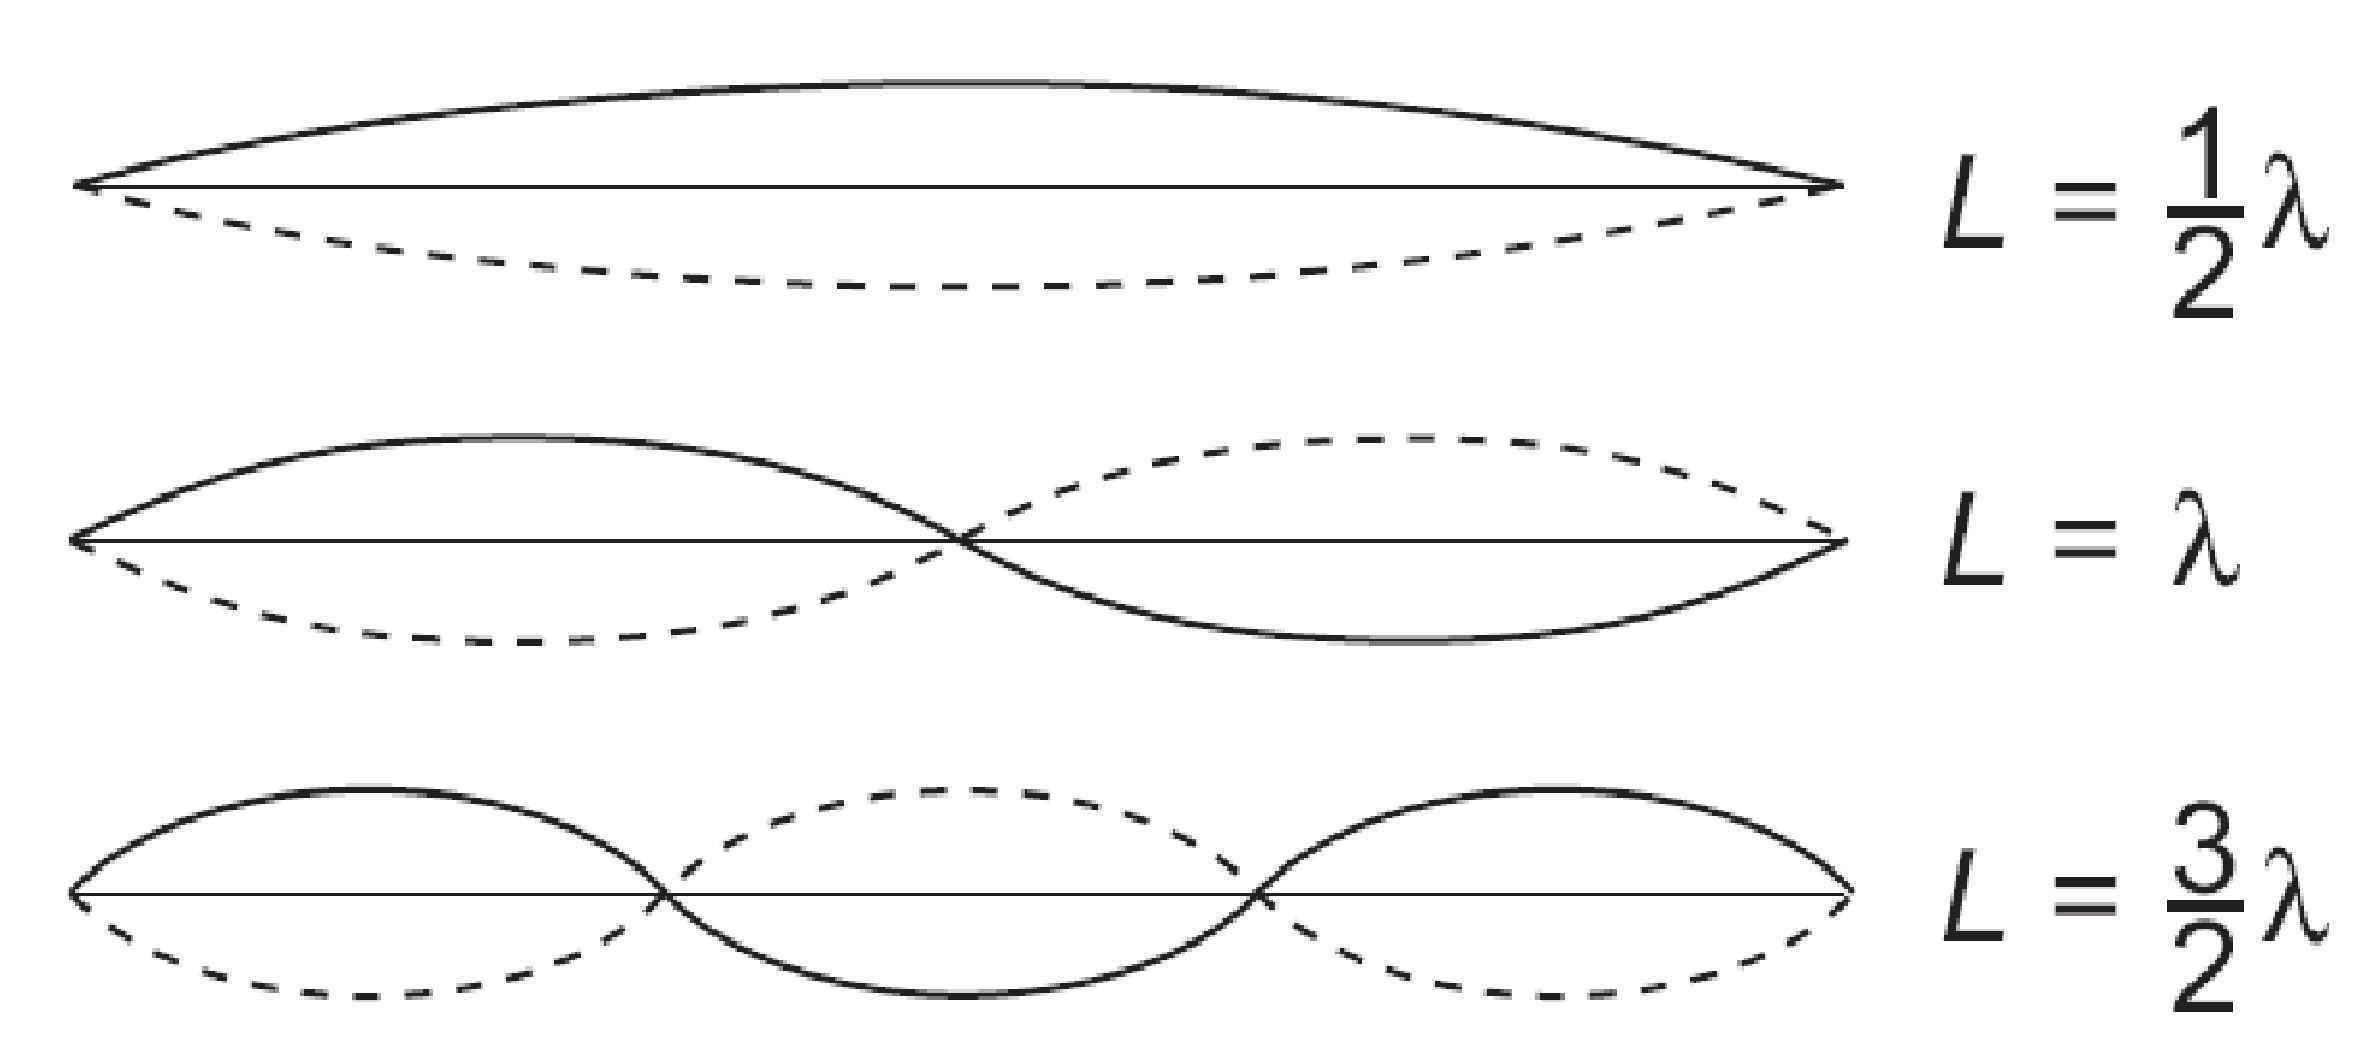
\includegraphics[width=3in]{Standing_waves_strings_fig1_tb.eps}
\end{center}
\vspace{0.3cm}

If you drive a stretched string at an arbitrary frequency, you will probably not see any particular mode; many modes will be mixed together. But, if the tension and the string's length are correctly adjusted to the frequency of the driving vibrator, one vibrational mode will occur at a much greater amplitude than the other modes.
For any wave with wavelength ($\lambda $) and frequency $f$, the speed, $v$, is:
\begin{equation}
v=\lambda f
\end{equation}

The speed of a wave on a string is also given by:
\begin{equation}
v=\sqrt{\frac {T}{\mu }}
\end{equation}
where $T$ is the tension in the string and $\mu $ is the linear density (mass/length) of the string.

In this experiment, standing waves are set up in a stretched string by the vibrations of an electrically-driven String Vibrator. The tension in the string equals the weight of the masses suspended over the pulley. You can alter the tension by
changing the masses. $L$ is the length of the string and $n$ is the number of segments. (Note that $n$ is not the number of nodes). Since a segment is 1/2 wavelength then


\begin{equation}
\lambda =\frac {2L}{n } \qquad n=1,2,3,...
\end{equation}



\vspace{0.3cm}
\begin{center}
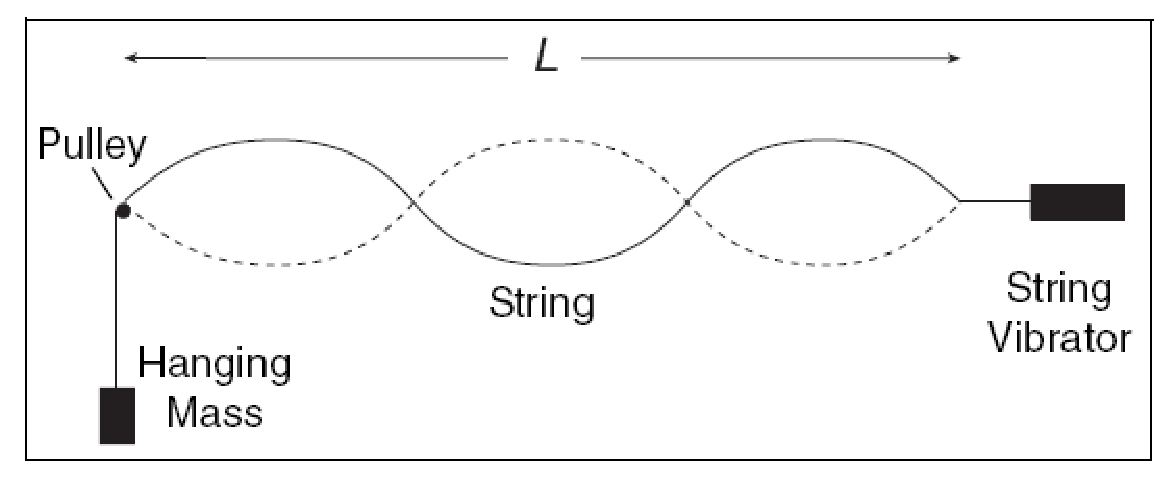
\includegraphics[width=250pt]{Standing_waves_strings_figure2.eps}
\end{center}
\vspace{0.3cm}


\textbf{Procedure}

\textbf{1. } Measure the exact length of a piece of string several meters long. Measure the mass of the
string and calculate the linear density (mass/length).(If your balance is not precise enough to measure that length of string, use a longer
piece of string to calculate the linear density.)

\vspace{2cm}

\textbf{2. } Clamp the String Vibrator and pulley about 100 cm apart. Attach the string to the vibrating blade, run it over the pulley, and hang about 200 g of mass from it. Cut off the excess string.

\textbf{3. } Measure from the knot where the string attaches to the String Vibrator to the top of the pulley.
This is the distance $L$. ($L$ is NOT the total length of the string that you measured in \textbf{1 }.) Record the value here: $L$ =

\vspace{0.3cm}
\begin{center}
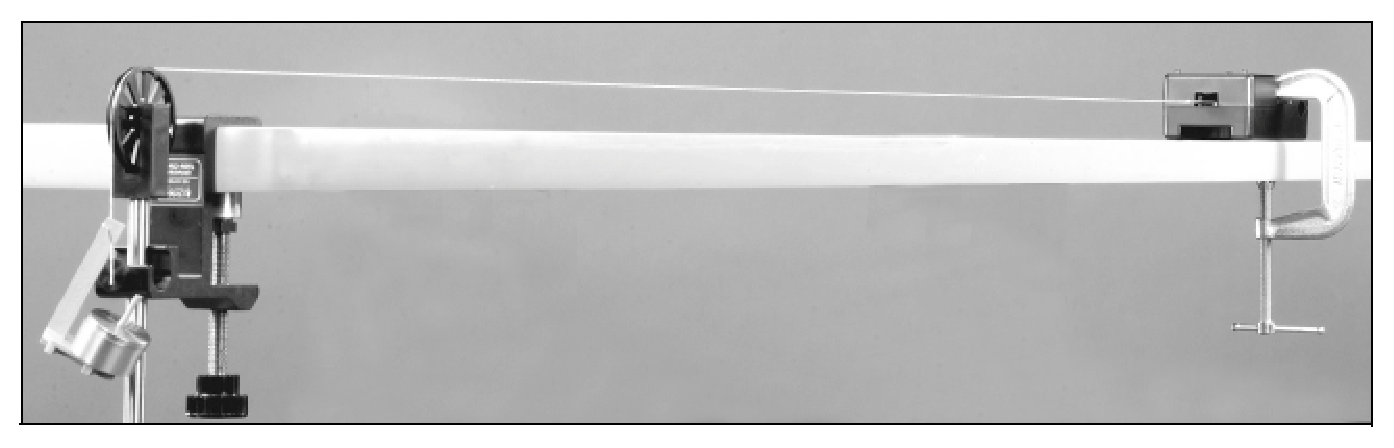
\includegraphics[width=320pt]{Standing_waves_strings_figure3.eps}
\end{center}
\vspace{0.3cm}

\textbf{4. } Connect the AC power supply to the String Vibrator.

\textbf{5. } Adjust the tension by adding to or subtracting from the hanging mass so that the string vibrates in 2 segments. Adjust the tension further to achieve a ``clean'' node at the center. Also check the end of the vibrating blade; the point where the string attaches should be a node. It is more important to have a good node at the blade than it is to have the largest amplitude possible. However, it is desirable to have the largest amplitude possible while keeping a good node.

\textbf{6. } Record the value of the hanging mass $m$ here:

\vspace{3cm}

\textbf{Part A: Speed of the Wave }

\textbf{a. } Calculate the tension in the string. (The weight of the hanging mass provides the tension in the string.)

\vspace{3cm}

\newpage

\textbf{b. } Calculate the speed $v_A$ of the wave from your observed values of tension ($T$) and linear density ($\mu $). Record your calculated value with the correct number of significant figures.


\vspace{4cm}

\textbf{c. } Calculate the speed $v_B$ from the wavelength ($\lambda $) and frequency ($f$). (In the U.S. $f$ = 60.0 Hz.)

\vspace{4cm}

\textbf{d. } Compare the two values ($v_A$ and $v_B$) of speed. What is the difference?

\vspace{4cm}

\textbf{e. } Calculate the percentage by which $v_A$ deviates from $v_B$.

\begin{equation}
\% Deviation =\frac {v_A - v_B}{v_B} \times 100\%
\end{equation}

\vspace{3cm}

\newpage

\textbf{Part B: Linear Density}

\textbf{a. } Produce standing waves of 3, 4, 5, etc. segments in the string. Get as many as you can. Record the mass, $m$, and the number of segments, $n$, in a table here. Be sure to include the results from Part A ($n$ = 2) in the table.

\vspace{6cm}

\textbf{b. } For every value of mass, calculate the tension in the string, and include in the above table.

\textbf{c. } In $Excel$, plot a graph of $T$ versus $n$ and include with this unit. Add a trendline with equation using a power function. What is the power of $n$?
\vspace{20mm}

\textbf{d. } For every value of $n$, calculate $\frac{1}{n^2}$ and include in above table. In $Excel$, plot a graph of $T$ versus $\frac{1}{n^2}$. Does the graph look linear? If so, include a linear trendline with equation. Print the graph and include with this unit.
\vspace{20mm}

\textbf{e. } Record the slope of the graph (including units) here:

\vspace{20mm}

\textbf{f. } Combine the equations in the \textbf{Background } section, and show that the tension can be written as:

\begin{equation}
T=4\mu f^{2}L^{2}\frac{1}{n^2}
\end{equation}

\vspace{25mm}

Thus the slope of a $T$ versus $\frac{1}{n^2}$ graph is $4\mu f^{2}L^{2}$.

\textbf{g. } Use the slope from your graph to calculate the density, $\mu $, of the string. Show that the units are kg/m.

\vspace{5cm}

\textbf{h. } Compare this measured value of string density to the accepted value. (You calculated the accepted value of $\mu $ from the mass and length of the string at the beginning of the experiment). Calculate a percent difference between the two values.

\vspace{50mm}

%\textbf{i. } Calculate the percent deviation of the measured value of $\mu $ from the accepted value.

%\begin{equation}
%\% Deviation =\frac{Measured-Accepted}{Accepted}\times 100\%
%\end{equation}

%\vspace{4cm}

\textbf{Further Investigation}

%\textbf{1. } Hang a mass on the string with a value that is about halfway between the masses that produced standing waves of 3 and 4 segments. The string should show no particular mode. Place a ``bridge'' so that you can see the exact fundamental ($n = 1$) between the String
%Vibrator and the bridge. What is the wavelength?

%\vspace{1.5cm}

%Slide the bridge away from String Vibrator until the string vibrates in 2 segments. How does the wavelength of the two-segment wave compare to the wavelength of the previous one segment wave?

%\vspace{1.5cm}

%Why is a standing wave created only when the bridge is at certain locations? What are these locations called?

%\vspace{1.5cm}

If a strobe is available, observe the standing wave on a string with the 
strobe light. Draw a diagram explaining the motion of the string.




 %132 equivalent

\section{Resonance in Tubes}

Name \rule{2.0in}{0.1pt}\hfill{}Section \rule{1.0in}{0.1pt}\hfill{}Date \rule{1.0in}{0.1pt}



{\noindent \bf Objectives:} \begin{list}{$\bullet$}{\itemsep0pt \parsep0pt}

\item Determine the resonant frequency for a tube open at one end.

\item Determine tube lengths at resonance for a tube of variable length.

\item Determine the velocity of sound in air in the laboratory (two ways).

\end{list}

\noindent {\bf Introduction} 

The Economy Resonance Tube is designed for the study of resonance in columns of air.  The tube set includes a movable inner tube with a closed end and an outer tube which is open at both ends.  The inner tube also includes a measuring tape to easily find the length of the air column in the outer tube. To adjust the length of the outer tube, simply slide the inner tube until the desired length appears on the measuring tape.  Open tube experiments can also be performed with the outer tube by removing the inner tube.

\noindent In order that the tube resonate, the frequency of the vibrating air must coincide with the natural frequency of the tube (which may be its fundamental or one of its overtones). For the Economy Resonance Tube, which is closed at one end, this requirement is met if the tube length is an odd number of quarter wavelengths of the sound waves produced by the source ($L = \lambda/4, 3 \lambda/4, 5 \lambda/4$, etc., where $L$ is the length of the tube and $\lambda$ is the wave length of the sound). Note that if the length of the tube is gradually increased while the source is vibrating, the distance between successive resonance positions is $\lambda/2$. \\

\noindent {\small {\bf Note:} Due to edge effects at the open end of a tube, the effective length of the tube depends on the radius of the opening. Thus, $L_{eff} = L + 0.6r$, where $L_{eff}$ is the \textit{effective} length, $L$ is the length measured, and $r$ is the tube radius.} \\


{\noindent \bf Apparatus:} \begin{list}{$\bullet$}{\itemsep0pt \parsep0pt}

\item Economy Resonance Tube 
\item Open speaker
\item Sine wave generator
\item 2 banana plug leads
\item Sound sensor
\item Meter stick
\item Data Studio 750 Interface
\item Thermometer

\end{list}

\noindent Room Temperature ($^\circ$C) \hrulefill \ \  Tube radius (m) \hrulefill

\vspace{5mm}

{\noindent \bf Activity 1: Fixed tube length} \begin{enumerate}

\item Connect the open speaker to the sine wave generator using standard banana plug leads.

\item Adjust the length of the outer tube to 50 cm (check with meter stick).

\item Place the tube in front of the speaker in such a way that the tube is open at one end (the speaker can be set at an angle relative to the tube length).

\item Set the sound sensor inside the tube and connect it to the Data Studio interface.

\item To activate the sound sensor, perform the following sequence:  Start up \textit{DataStudio} by going to \textit{Start} $\rightarrow$ \textit{Programs} $\rightarrow$ \textit{Physics Applications} $\rightarrow$ \textit{DataStudio}.
Click on \textit{Create Experiment}, then \textit{Setup}, then \textit{Add Sensor or Instrument}. Scroll down to \textit{Sound level sensor} and select, then click \textit{OK}. Double click \textit{Graph} at left. Click \textit{Start} to begin taking data.

\item Start at a frequency of 130 Hz and increase until you find the frequency of the largest resonance (indicated by a peak on the sound level graph).  This is the fundamental frequency.  Record the result here:\vspace{10mm}

\item The resonant frequencies for a tube open at one end are given by $f=nv/4L$ where $n$ is an odd integer, $v$ is the velocity of sound and $L$ is the effective tube length.  From the fundamental frequency you just found, calculate the velocity of sound in air (using $n$ = 1) and record it here:\vspace{15mm}

\end{enumerate}

%\noindent {\Large{\bf DATA}} \\

%\noindent Room Temperature ($^\circ$C) \hrulefill \ \  Tube radius (m) \hrulefill

%\begin{center} \begin{tabular}{||c|c|c|c|c|c|c|c|c|c|c|c|c|c|c||} \hline \hline Tuning Fork & \multicolumn{4}{|c|}{First Position of} & \multicolumn{4}{|c|}{Second Position} & \multicolumn{4}{|c|}{Third Position of} & Wave- & Velocity of \\ Frequency, & \multicolumn{4}{|c|}{Resonance, m} & \multicolumn{4}{|c|}{of Resonance, m} & \multicolumn{4}{|c|}{Resonance, m} & length, & Sound in \\ \cline{2-13} Hz & 1 & 2 & 3 & Ave. & 1 & 2 & 3 & Ave. & 1 & 2 & 3 & Ave. & m & air, m/s \\ \hline \hline &&&&&&&&&&&&&& \\ \hline &&&&&&&&&&&&&& \\ \hline \hline \end{tabular} \end{center}


{\noindent \bf Activity 2: Fixed frequency} \begin{enumerate}

\item Adjust the outer tube length to 20 cm.

\item Set the speaker inside the open end of the tube so that it is closed at both ends.

\item Set the sine wave generator frequency to 600 Hz (with low amplitude).

\item Slowly move the inner tube to increase the effective length of the tube.  Record the length of the tube when resonance is achieved. You don't need to use the sound sensor for this. Just listen for maximum loudness.\vspace{10mm}

\item Increase the length of the tube until two more resonance lengths are found for the constant frequency and record them here:\vspace{15mm}

%\item Average your two values to determine your experimental velocity of sound in m/s: \ \ \  \rule{2cm}{1pt}

\item The maxima you have determined are spaced a distance $\lambda/2$ apart, where $\lambda$ is the wavelength.  Find the differences between adjacent resonance lengths and calculate the average of the two values:\vspace{15mm}

\item Find $\lambda$ from your average value of $\lambda/2$ and calculate the velocity of sound in air from $v=f\lambda$.\vspace{15mm}

\item The velocity of sound in air at $0^\circ$C is 331.4 m/s.  The temperature dependence of sound velocity in air is given by $v(T) = 331.4 + 0.6T$, where $T$ is in $^\circ$C and $v$ is in m/s. Calculate an ``accepted'' value of the velocity of sound in air from this formula.

\vspace{15mm}

\item What is the percent difference between your experimental result and the ``accepted'' value?

\end{enumerate}
 %132 equivalent

%--------------------------------------------
\part{Electricity and Magnetism}


\section{Electrostatics}

Name \rule{2.0in}{0.1pt}\hfill{}Section \rule{1.0in}{0.1pt}\hfill{}Date
\rule{1.0in}{0.1pt}

\textbf{Objective}

\begin{itemize}
\item To understand the basic phenomena of electric charges at rest.
\end{itemize}
\textbf{Introduction}

Atoms consist of a central nucleus made up of protons and neutrons
surrounded by one or more electrons. While the nuclei of solids are
essentially localized, some of the electrons may be free to move about.
A substance which has as many electrons as it has protons is said
to be electrically neutral. Dissimilar objects have different affinities
for electrons. When two such objects, initially neutral, are rubbed
together, the friction may cause electrons to pass from one to the
other. After separation, neither object is neutral. Each is said to
have been {}``charged by friction''. An isolated, electrified object
becomes neutral again if its electron-proton balance is restored.
A convenient means for accomplishing this is to connect the object
to earth by means of a conductor, through which electrons readily
travel. This process is called {}``grounding the body''. Since an
electrified object is referred to as {}``charged'', grounding is
also referred to as {}``discharging''.

Substances through which electrons do not move easily are called {}``non-conductors'',
or {}``insulators''. Experiment has shown that when rubber and wool
are rubbed together, electrons pass form the wool to the rubber. The
electrons remain on the surface of the rubber--a non-conductor--where
they were transferred.

Rubbing a metal rod with a wool cloth can also transfer electrons.
This rod, however, is a conductor and electrons pass through it to
the experimenter and then to the earth. People, made mostly of salt
water, are good conductors, as well. Metal that is isolated, however,
can be electrified. This can be demonstrated with an electroscope,
which has a metal knob connected to a stem from which a thin metal
leaf hangs. An insulator prevents contact of these metal parts with
the case, and consequently the earth.

\textbf{Apparatus}

\begin{itemize}
\item electroscope
\item rubber and glass rods
\item wool and silk cloth
\item plastic rod with metal disk mounted on one end
\end{itemize}
\textbf{Activity 1: Charging by Friction}

\begin{enumerate}
\item Be sure the electroscope is discharged by touching the knob with your
finger. Explain what happened and why you are convinced the electroscope
is discharged.\vspace{15mm}

\item \textbf{Prediction:} If you rub the knob of an electroscope with a
wool cloth, what will be the state of the electroscope when you remove
the cloth? Explain.\vspace{15mm}

\item Gently and repeatedly rub the knob of the electroscope with the wool cloth for a couple of minutes. Remove the cloth. Note any differences in the electroscope from its appearance before you rubbed.\vspace{15mm}

\item Explain what, if anything, happened.\vspace{15mm}

\end{enumerate}
\textbf{Activity 2: Charging by Contact}

\begin{enumerate}
\item Discharge the electroscope as before.
\item Charge the plastic rod by friction with
the wool cloth.
\item Does anything occur in the electroscope when you bring the disc close
to the knob without touching it?\vspace{15mm}

\item \textbf{Prediction:} What will happen to the electroscope if you repeatedly
touch its knob with a freshly charged object?\vspace{15mm}

\item Touch the disc to the knob; rub the disc again and again touch it
to the knob; repeat this procedure two or three more times. Describe
any changes to the electroscope.\vspace{15mm}

\item Repeat the procedure above until the electroscope's leaf is at approximately
a twenty degree angle with the stem.
\end{enumerate}
\textbf{Activity 3: Kinds of Electrification}

\begin{enumerate}
\item Electrify one end of the rubber rod by wrapping the wool cloth around
the rod, squeezing the wool against the rod, twisting the rod vigorously
to ensure good contact, and separating the wool from the rod.
\item \textbf{Prediction:} What will happen when you bring the electrified
end of the rubber rod toward, but not touching, the electroscope's
knob? What will happen if you do the same with the wool cloth?\vspace{15mm}

\item Bring the charged end of the rubber rod toward the knob, but do not
touch it. Record what happens.\vspace{15mm}

\item Repeat number 3 with the wool cloth.\vspace{15mm}

\item What differences were there between the trial with the rod and the
trial with the cloth?\vspace{15mm}

\item How would you account for these differences?\vspace{15mm}

\item \textbf{Note:} By definition, the electrical state of the rubber after
being rubbed by the wool is negative. That is, an object that has
an excess of electrons is said to be negatively charged. Realize that
this is only a convention.
\item If the rubber is said to be negatively charged, in what electrical
state is the wool cloth?\vspace{15mm}

\item How can an electroscope be used to determine the nature of any charge?\vspace{15mm}

\item Rub the end of the glass rod with the silk cloth and determine the
charge of each (positive or negative) after they are separated.\vspace{15mm}

\end{enumerate}
\textbf{Activity 4: Action of the Electroscope}

\begin{enumerate}
\item \textbf{Discussion:} Two facts explain the rise or fall of the leaves
of an electroscope: (a) Like charges repel (unlike charges attract);
and (b) Free electrons move about in a conductor when an electric
force acts upon them.
%\item Discharge the electroscope.
%\item \textbf{Prediction:} What will happen when you bring the charged rubber
%rod near the discharged electroscope? What will happen if you do the
%same with the wool cloth?\vspace{15mm}

%\item Test your predictions; record the results; try to explain them.\vspace{15mm}

\item When the wool cloth approaches the knob (in Activity 3 number 4), which way do the free electrons
in the metal of the electroscope move (up toward the knob or down
toward the leaf)?\vspace{15mm}

%\item Do the leaf and stem now become positive or negative?\vspace{15mm}

\item In Activity 3, the electroscope was negatively charged before either
the rod or the wool was brought toward the knob. For the case of the
rod, in which direction do the free electrons in the electroscope
move? Does the electron displacement increase or decrease the electrostatic
force separating the leaf from the stem?\vspace{15mm}

\end{enumerate}
\textbf{Activity 5: Charging by Induction}

\begin{enumerate}
\item Discharge the electroscope.
\item \textbf{Prediction:} What will be the effect on the electroscope if
you perform the following experiment: while grounding the electroscope
with your finger, bring an electrified rubber rod near the knob, then
take away your finger and then the rod (in that order)?\vspace{15mm}

\item Carry out the experiment and describe the result.\vspace{15mm}

\item Explain the result and why your prediction agreed or disagreed with
it.\vspace{15mm}

\item \textbf{Prediction:} Note that no electrons moved between the rod
and the electroscope. What charge has been induced on the electroscope?\vspace{15mm}

\item Test your prediction with the negatively charged rubber rod and the
positively charged wool.
\item Does the test verify or contradict your prediction?\vspace{15mm}
\end{enumerate}

 %132 equivalent
%
\section{Electric Fields and Equipotential Lines}

Name \rule{2.0in}{0.1pt}\hfill{}Section \rule{1.0in}{0.1pt}\hfill{}Date
\rule{1.0in}{0.1pt}

\textbf{Objective}

\begin{itemize}
\item To learn the shape of electric fields.
\end{itemize}
\textbf{Introduction}

Charged objects exert an electrical force on other charged objects
in proportion to the amount of charge each has, just as massive objects
exert a gravitational force on one another in proportion to their
masses. The magnitudes of both forces depend, too, on the distance
between objects. However, whereas the gravitational force is always
attractive, electrical forces may be either attractive or repulsive
depending on the sign of the charges. It is convenient in understanding
the nature of electrical forces to draw pictures of them. We represent
the fields, which provide the magnitude and direction of the forces,
as lines. We agree on a convention: the direction of the field is
that of the force on an infinitesimal positive test charge. Thus,
the lines of force originate on and come out of positive charges and
are directed toward and terminate on negative charges (see figure
below). The magnitude of the field, and therefore the force, is proportional
to the density of the field lines.

\vspace{0.3cm}
{\centering 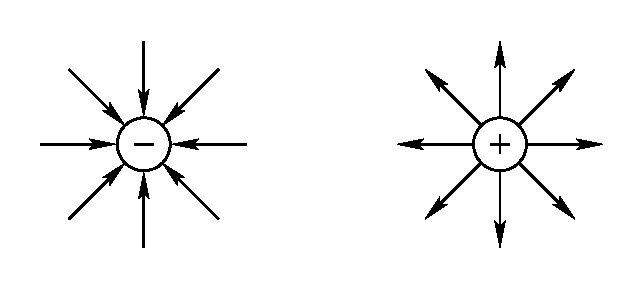
\includegraphics{ef_equipot_lines_fig_1.eps} \par}
\vspace{0.3cm}

Please note that when the situation is electrostatic, 1) the electric
field within a metal is zero, and 2) the electric field just outside
the surface of a metal is perpendicular to the surface. If either
of these conditions were altered, then there would be an electric
current in the metal, which is not an electrostatic situation. Because
an electric field exerts a force on a charge, work must be done to move a
charged object along any of the field lines. On the other hand, movement
perpendicular to the field lines requires no work. Such movement is
said to be along an equipotential line.

\vspace{0.3cm}
{\centering 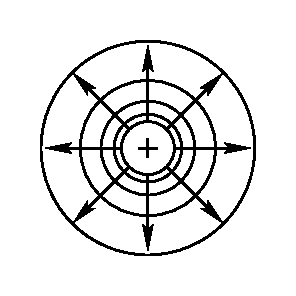
\includegraphics{ef_equipot_lines_fig_2.eps} \par}
\vspace{0.3cm}

In the figure above, the electric field for a positive point charge
is shown as lines with arrows. The regions of equipotential (equipotential
lines) are shown with circles. Notice that the equipotential lines
are perpendicular to the electric field lines and that the density
of equipotential lines is proportional to the electric field strength.

Electric field lines are difficult to measure directly, but potentials
can be measured with a voltmeter. An electric field will arise in
the space surrounding two separated charged conductors. With one lead
of a voltmeter connected to one of the conductors and the other used
as a probe, the potentials can be determined (see figure below).

\vspace{0.3cm}
{\centering \resizebox*{0.9\textwidth}{!}{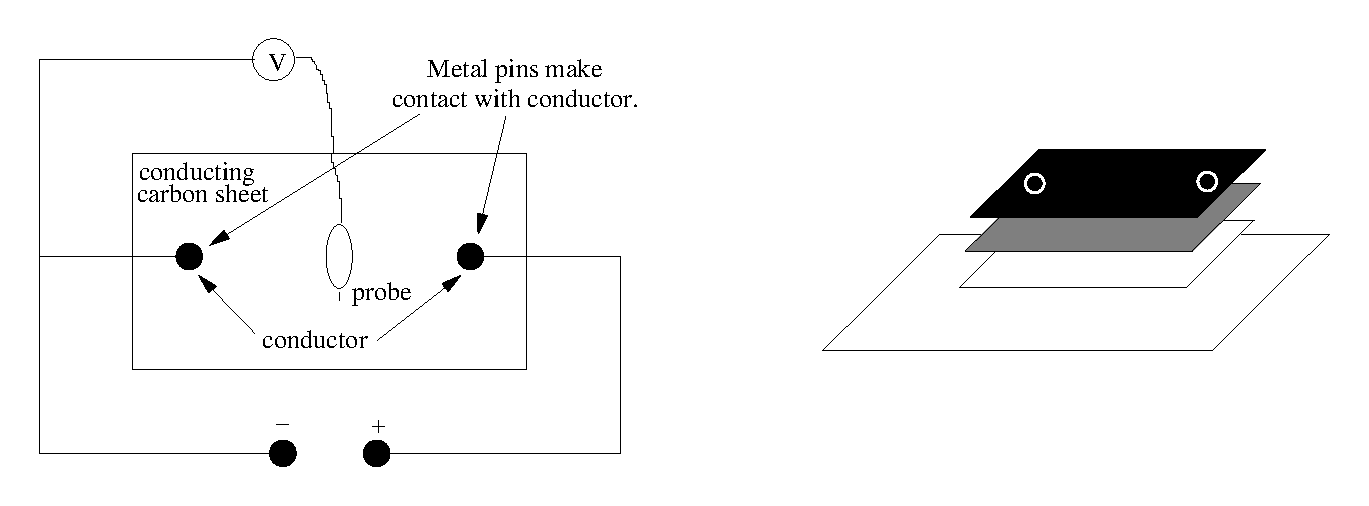
\includegraphics{ef_equipot_lines_fig_3.eps}} \par}
\vspace{0.3cm}

\textbf{Apparatus}

\begin{itemize}
\item Power supply
\item Voltmeter
\item Conducting sheets
\item Carbon and white paper
\item Wooden board and pins
\end{itemize}
\textbf{Activity 1: Field Lines for Two Point Charges}

\textbf{Prediction:} Using the rules given in the introduction and
given in the first set of figures, draw the electric lines for two
oppositely charged point objects. Sketch the equipotential lines.
\vspace{1in}

\begin{enumerate}
\item Find the conducting paper with the two silver circles on the front
and lay it over a copy carbon and a sheet of paper on top of the wooden
board.
\item Connect the positive output of the power supply to one of the circles
and the negative to the other.
\item Connect the negative lead of the voltmeter to the negative conductor
and use the positive lead as the probe. 
\item With the power supply voltage turned on and set to 10 volts, probe
lightly with the voltmeter to find a number of points on the carbon
paper registering 8 volts. Push down each time you find a point so
that marks will be made on the bottom paper.
\item Repeat for 6 volts, 4 volts, and 2 volts.
\item You should end up with a series of dots on your sheet of paper. Connect
those associated with the same potential with smooth lines.
\item Recalling the relationship between electric field lines and equipotential
lines, sketch in the electric field lines. (\emph{Other group members
can sketch copies of the same results.})
\item Does your experimental result agree with your prediction? Explain.\vspace{15mm}

\end{enumerate}
\textbf{Activity 2: Field Lines for Parallel Plates}

\textbf{Prediction:} Draw what you think the field lines and equipotential
lines between parallel plates will look like.
\vspace{1in}

\begin{enumerate}
\item Carry out the instructions from Activity 1 to check your prediction.
\item Does your result agree with your prediction? Explain.\vspace{15mm}

\end{enumerate}
\textbf{Activity 3: Field Lines Between a Point Charge and a Plate}

\textbf{Prediction:} Draw what you think the field lines and equipotential
lines between a point charge and a parallel plate will look like.
\vspace{1in}

\begin{enumerate}
\item Map the field lines as before.
\item Does your result agree with your prediction? Explain.\vspace{15mm}

\item If the potential is zero, must the electric field be zero as well?\vspace{15mm}

\item What can you say about the electric field along an equipotential line?\vspace{15mm}

\end{enumerate}
%\textbf{Activity 4: Field Lines for a Plate and a Charged Circle}

%\textbf{Prediction:} Sketch what you think the field and potential
%lines between a charged circle and a plate look like.
%\vspace{1in}

%\begin{enumerate}
%\item Determine the field lines.
%\item What is the field strength within a charged, continuous surface?\vspace{15mm}
%\end{enumerate}



\section{The Electric Field and the Electric Potential I}

Name \rule{2.0in}{0.1pt}\hfill{}Section \rule{1.0in}{0.1pt}\hfill{}Date
\rule{1.0in}{0.1pt}

\textbf{Objective}

\begin{itemize}
\item To investigate the electric field and potential of a point charge.
\end{itemize}

\textbf{Apparatus}

\begin{itemize}
\item Electric field and potential simulation entitled {\it EMField}.
\end{itemize}

\textbf{Introduction}

The direction of an electric field is the direction of the force on
a tiny positive test charge placed in the region of space where the
field is to be measured. If the magnitude of this test charge is infinitesimally
small, so small that it will not displace or disturb the charges that
are the source of the field, we can use the test charge to determine
quantitatively the strength of the electric field. The strength of
the electric field is taken to be the electric force, $F$, on the test
charge divided by the magnitude of the test charge, \( q_{t} \):
\( E=\frac{F}{q_{t}} \). The force (Coulomb's Law) between two charges,
\( q_{1} \) and \( q_{2} \), is \( F=k\frac{q_{1}q_{2}}{r^{2}} \),
where \( k \)= 9 x 10\( ^{9} \) Nm\( ^{2} \)/C\( ^{2} \). The units
of \( E \) are newtons per coulomb, so another way of describing the field
strength is to say it is the force experienced by a unit positive
test charge.

Recall from a previous laboratory exercise that the potential difference
between two points A and B, V\( _{B} \) - V\( _{A} \), is the work
done carrying a unit positive charge from point A to point B. Also,
the lines of force (the electric field lines) are always perpendicular
to the equipotential lines, lines on which all points are at the same
potential. In a static electric field, the electric potential difference
between two points is a constant and does not depend on the path used
for its computation. The absolute potential, as opposed to the potential
difference, is the amount of work done in carrying a unit charge from
infinity to point B. The magnitude of the absolute potential, then,
is computed as the integral from infinity to the point B of the electric
field.

\textbf{Investigation 1: A Single Charge}

\textbf{Activity 1: The Electric Field}

(a) Start the program {\it EMField} from the {\it Physics Applications} menu.
Click on the screen and you will see a screen with a set of
instructions.
Go to the \textbf{Sources} menu and select \textbf{3D Point Charges}.
A blank `table top' with a set of menu 
buttons at the top and bottom will appear. See Figure 1 below.

\begin{figure}[hbt]
\begin{center}
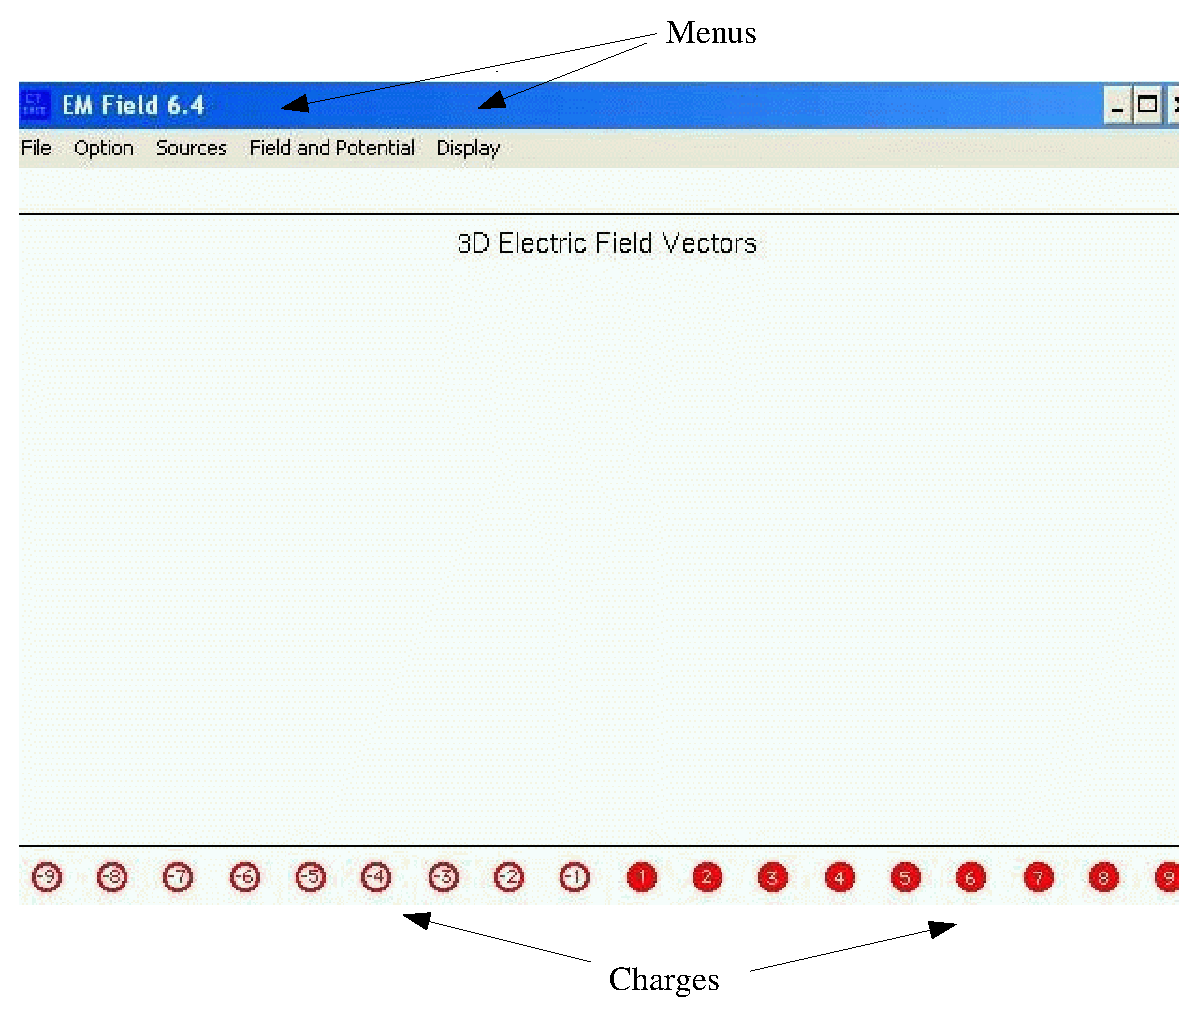
\includegraphics[height=4.0in]{emfield1c.eps}
\caption{Table top for {\it EMField.}}
\end{center}
\end{figure}

(b) Go to the {\bf Display} menu and set {\it EMField} to
{\bf Show Grid} and {\bf Constrain to Grid}.
These choices will make the following investigation a bit easier to perform.

(c) Select
the charge labeled {}``+4'' from the available set by clicking
on it and dragging it to the center of the table top. 

(d) \textbf{Prediction}: You will take measurements of the field at different
distances from the charge. You know the relative size of the
charge (+4), but you don't know the size of the charge in coulombs.
Generate an expression for the magnitude of the field from an unknown charge
with appropriate numerical constants and units.
The only unknown in your result should be the charge in coulombs.
How does the electric field depend on $r$, the distance from the point charge?
%\vspace{15mm}
\newpage

(e) Click anywhere in the table top and you will see an arrow drawn.
The size and direction of the arrow represent the magnitude and direction of
the electric field at that point due to the `+4' charge.
In what direction does the arrow point?
Click on the opposite side of the table top.
In what direction does this arrow point? How is it related to the first arrow?
\vspace{15mm}

(f) Click on many points so that you get a wide range of magnitudes from large
(barely fits on the table top) to small (barely bigger than a dot).

(g) Print the table top and use a ruler to measure the distance of each field 
point from the charge and the lengths of each of the arrows on your plot. 
Enter these data in the table below. Use the scale at the bottom of the table 
top to convert the length of each arrow into an electric field magnitude.
The units of the scale electric field vector are $1.0 ~ N/C$.

\vspace{0.3cm}
{\centering \begin{tabular}{|c|c|c|c|}
\hline 
~~~Distance from Charge (m)~~~&
~~~Arrow Length (cm)~~~&
~~~Measured E (N/C)~~~&
~~~Charge (C)~~~\\
\hline
\hline 
&
&
&
\\
\hline 
&
&
&
\\
\hline 
&
&
&
\\
\hline 
&
&
&
\\
\hline 
&
&
&
\\
\hline 
&
&
&
\\
\hline 
&
&
&
\\
\hline 
&
&
&
\\
\hline 
&
&
&
\\
\hline
\end{tabular}\par}
\vspace{0.3cm}

(h) Use the results in column 3 of your table to determine the unknown charge for each electric field measurement and enter the results in the table. NOTE: 
For this calculation, assume the Coulomb's Law constant $k = 1.00 Nm^{2}/C^{2}$.
This makes the charge a factor of about $10^{10}$ bigger than it is supposed to 
be, but we are focussing here on how the electric field varies with distance 
from the charge. Calculate the average and standard deviation of the values 
of the charge. Are your results consistent? Explain.
\vspace{30mm}

(i) \textbf{Prediction}: From Coulomb's Law, we expect the spatial variation
of the field strength to obey a power law: \( \left| E\right| =Ar^{n} \),
where \( A \) and \( n \) are constants. What do you predict the value of \( n \) to be?\vspace{15mm}

(j) Graph field strength as a function of $r$. Using the power fitting
function, determine the power of the function, $n$, and record it here.
Attach the plot to this unit.
\vspace{15mm}

(k) Does your result agree with your prediction? Explain any discrepancy.
\vspace{15mm}

\vspace{0.5in}
\textbf{Activity 2: The Electric Potential}

(a) Under the {\bf Display} menu click on {\bf Clean up Screen} to erase the
electric field vectors.

(b) \textbf{Prediction}: You will now take measurements of the potential.
How do you expect the electric potential to change with distance from the point
charge?
\vspace{15mm}
 
(c) Click on the \textbf{Potential} option under the \textbf{Field and Potential} menu. Click on the table top and a marker will be
placed at that point and labeled with the value of the potential there.
Click on many spots on the table top from very close to the point charge to
far away.
When you are finished print the table top.
\vspace{5mm}

(d) Measure and record in the following table the values of the distance from the point charge and the potential.

\vspace{0.3cm}
{\centering \begin{tabular}{|c|c|}
\hline 
~~~Distance (m)~~~&
~~~Measured V (volts)~~~\\
\hline
\hline 
&
\\
\hline 
&
\\
\hline 
&
\\
\hline 
&
\\
\hline 
&
\\
\hline 
&
\\
\hline 
&
\\
\hline 
&
\\
\hline 
&
\\
\hline
\end{tabular}\par}
\vspace{0.3cm}


%(e) Calculate the value of the electric potential at each of these points
%from the distance you measured from the point charge and the value of the 
%charge from the previous activity. Again, assume $k = 1.00 Nm^{2}/C^{2}$.
%Fill in the appropriate columns of the table  with the distance
%and predicted potential. Show a sample calculation in the space below.
%\vspace{1in}


%(f) Did the measured values agree with your calculations? If they didn't,
%can you explain why not?\vspace{25mm}

(e) \textbf{Prediction}: From Coulomb's Law and the definition of the
electric potential, we expect the spatial variation of the potential
to obey a power law: \( \Delta V=Br^{m} \), where \( B \) and \( m \)
are constants. What do you predict the value of \( m \) to be?
\vspace{12mm}

(f) Graph the voltage as a function of $r$. Using the power fitting
function, determine the power of the function, $m$, and record it here.
\vspace{12mm}

(g) Does your result agree with your prediction? Explain any discrepancy.
\vspace{12mm}

\textbf{Activity 3: Field Lines and Equipotentials}

(a) Under the {\bf Display} menu click on {\bf Clean up Screen} to erase the 
potential values.

(b) Click on {\bf Field Lines} under the {\bf Field and Potential} menu. Click on many spots on the table top all around the charge to create field lines. Why are they straight lines?
\vspace{15mm}

(c) Click on {\bf Directional Arrows} under the {\bf Field and Potential} menu. Click on many spots to create directional arrows for the field lines. (Remember, electric field is a vector quantity.) Why are they directed away from the charge?
\vspace{15mm}

(d) Click on {\bf Equipotentials} under the {\bf Field and Potential} menu. Click on many spots to create equipotential lines. Why are they all circular?
\vspace{15mm}

(e) What is the relationship between the field lines and the equipotentials at 
the points where they cross?
 %132 equivalent

\section{The Electric Field and the Electric Potential II}

Name \rule{2.0in}{0.1pt}\hfill{}Section \rule{1.0in}{0.1pt}\hfill{}Date
\rule{1.0in}{0.1pt}

\textbf{Objective}

\begin{itemize}
\item To investigate the electric field and potential of a charge distribution.
\end{itemize}

\textbf{Apparatus}

\begin{itemize}
\item Electric field and potential simulation entitled {\it EMField}.
\end{itemize}

\textbf{Introduction}

In the previous unit (which we will refer to as Investigation 1) we studied the dependence
of the electric field and the electric potential on $r$, the distance from a
single charge.
Now we will study the same ideas for a different charge distribution.

\textbf{Investigation 2: Four Symmetrically Arranged Charges}

\textbf{Activity 1: The Electric Field}

(a) Start the program {\it EMField} from the {\it Physics Applications} menu or (if it's already running) use the options under the 
\textbf{Display} menu to clear the table top and delete any charges.
Go to the \textbf{Sources} menu and select \textbf{3D Point Charges}.
A blank `table top' with a set of menu 
buttons at the top and bottom will appear (see Figure 1 in Investigation 1, the previous unit).

(b) Go to the \textbf{Display} menu and set {\it EMField} to
{\bf Show Grid} and {\bf Constrain to Grid} if they are not already set.
These choices will make the following investigation a bit easier to perform.

(c) Under \textbf{Sources}, click on \textbf{3D Point Charges}. Select the
charge labeled {}``+4'' from the available set by clicking on it.
Add four individual charges, arranging them symmetrically within about
1 cm of the central point where the {}``+4'' charge was located
in Investigation 1 (the previous unit). 

(d) {\bf Prediction:} How will the electric field be oriented within the region of the four charges?
How will the field be oriented outside the region of the four charges?
How will the field depend on $r$, the distance from the center of the four charges, at large $r$?
\vspace{25mm}

(e) Click anywhere in the table top and you will see an arrow drawn.
The size and direction of the arrow represent the magnitude and direction of
the electric field at that point due to the four charges.
In what direction does the arrow point?
Click on the opposite side of the table top.
In what direction does this arrow point? How is it related to the first arrow?
\vspace{15mm}

(f) Click on many points so that you get a wide range of magnitudes from large
(barely fits on the table top) to small (barely bigger than a dot).

(g) Print the table top and use a ruler to measure the lengths of each of the arrows on your plot, for points \textbf{outside} the region of the four charges. Enter this data in the following table. Use the scale at the bottom of the table top to convert the length of each arrow into an electric field magnitude.
The units of the scale electric field vector are $1.0 ~ N/C$.

\vspace{0.3cm}
{\centering \begin{tabular}{|c|c|c|}
\hline 
~~~Distance from Charge Center (m)~~~&
~~~Arrow Length (m)~~~&
~~~Measured E (N/C)~~~\\
\hline
\hline 
&
&
\\
\hline 
&
&
\\
\hline 
&
&
\\
\hline 
&
&
\\
\hline 
&
&
\\
\hline 
&
&
\\
\hline 
&
&
\\
\hline 
&
&
\\
\hline 
&
&
\\
\hline
\end{tabular}\par}
\vspace{0.3cm}


(h) \textbf{Prediction}: From Coulomb's Law, we expect the spatial variation
of the field strength to obey a power law: \( \left| E\right| =Ar^{n} \),
where \( A \) and \( n \) are constants. What do you predict the
value of \( n \) to be?\vspace{15mm}

(i) Graph your results. Using the power fitting
function, determine the power of the function, $n$, and record it here.
Attach the plot to this unit.
\vspace{15mm}

(j) Does your result agree with your prediction? Explain any discrepancy.\vspace{15mm}

\textbf{Activity 2: The Electric Potential}

(a) Under the {\bf Display} menu click on {\bf Clean up Screen} to erase the
electric field vectors.

(b) \textbf{Prediction}: You will now take measurements of the potential.
How do you expect the electric potential to change with distance from the center of the four charges?
\vspace{15mm}
 
(c) Click on the \textbf{Potential} option under the \textbf{Field and Potential} menu. Click on the table top and a marker will be
placed at that point and labeled with the value of the potential there.
Click on many spots on the table top from very close to the charges to
far away.
When you are finished print the table top.
\vspace{15mm}

(d) Measure and record in the following table the values of the distance from the center of the point charge region (for points outside the region of the four charges) and the potential.

\vspace{0.3cm}
{\centering \begin{tabular}{|c|c|c|}
\hline 
~~~Distance from Charge Center (m)~~~&
~~~Measured V (volts)~~~\\
\hline
\hline 
&
\\
\hline 
&
\\
\hline 
&
\\
\hline 
&
\\
\hline 
&
\\
\hline 
&
\\
\hline 
&
\\
\hline 
&
\\
\hline 
&
\\
\hline
\end{tabular}\par}
\vspace{0.3cm}


(e) \textbf{Prediction}: From Coulomb's Law and the definition of the
electric potential, we expect the spatial variation of the potential
to obey a power law: \( \Delta V=Br^{m} \), where \( B \)
and \( m \) are constants. What do you predict the value of \textbf{\( m \)}
to be?\vspace{15mm}


(f) Graph your results. Using the power fitting
function, determine the power of the function, $m$, and record it here.
\vspace{15mm}

(g) Does your result agree with your prediction? Explain any discrepancy.\vspace{15mm}

(h) How do your results for the power constants, $n$ and $m$, of the four
symmetrically-arranged charges compare with the power constants you
determined in Investigation 1 (the previous unit) for the single point charge?\vspace{15mm}

(i) What can you conclude about the field and potential effects due to
a distribution of charge outside the region of the distribution (in
relation to a single point charge)?\vspace{15mm}

 %132 equivalent

\section{Ohm's Law}

Name \rule{2.0in}{0.1pt}\hfill{}Section \rule{1.0in}{0.1pt}\hfill{}Date
\rule{1.0in}{0.1pt}

\textbf{Objectives}

\begin{itemize}
\item To investigate the most important principle in electronics.
\item To determine how resistors in series and parallel add.
\end{itemize}
\textbf{Introduction}

The rate at which electric charge flows through a conductor is called
the electric current. In order to have a current, a potential difference,
or voltage is necessary. We first want to determine the relationship
between the potential difference at two ends of a conductor and the
current flowing through it.

\textbf{Note}: Do not turn on a power supply until you are sure your
circuit is correct. If you are at all unsure, please ask your instructor
to approve your setup. Ammeters can be instantly and permanently ruined
by an improper connection. Be sure to turn off the power supply before
making any changes to the circuit.

\textbf{Apparatus}

\begin{itemize}
\item Power supply
\item Two resistors
\item Leads and alligator clips
\item DC Milliammeter
\item Multimeter
\end{itemize}
\textbf{Activity 1: Ohm's Law}

\begin{itemize}
%\item Connect two rheostats (or variable resistors) in series as shown in
%the figure below. Set R\( _{1} \) at about the halfway point and
%R\( _{2} \) at the maximum. Connect an ammeter as shown. Also, connect
%a voltmeter across (that is, connect a probe to each side of) R\( _{1} \).
%\item The fixed resistor will be considered an ``unknown'' and will be called 
%R\( _{1} \). The variable resistor will be called R\( _{2} \), and will be used 
%to vary the current. Connect the two resistors in series as shown in the 
%figure. Set R\( _{2} \) at its maximum value. Connect a milliammeter as shown, 
%at the point marked ``A'' (for ``ammeter''). Leave the positive lead to the 
%power supply disconnected.
\item With the power supply off, turn the coarse current control all the way up 
and both voltage controls all the way down.  Connect one of the resistors in 
series with the milliammeter (marked ``A'' for ``ammeter'') as shown in the 
figure below. Be sure the polarity of the milliammeter is as shown.
\end{itemize}
\vspace{0.3cm}
{\centering \resizebox*{0.35\textwidth}{!}{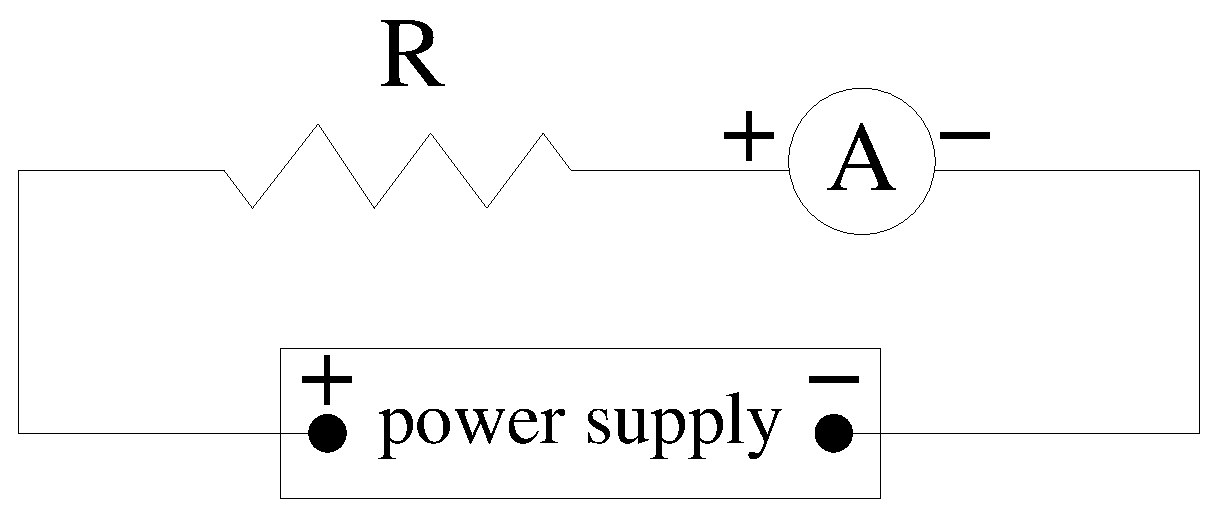
\includegraphics{ohms_law_fig_3.eps}} \par}
\vspace{0.3cm}

\begin{itemize}
\item When sure of your circuit, turn on the power supply, and turn the coarse 
voltage control up until the milliammeter reads 20 ma. Measure the voltage 
across the resistor (with the multimeter set for DC voltage) and record both voltage and current here:
\vspace{10mm}

%\item Reduce the resistance of R\( _{2} \) and record the current and voltage
%three more times by turning down R\( _{2} \) in approximately equal steps so 
%that for the last time R\( _{2} \) is turned completely down. 
%Record your results here:\vspace{30mm}

\item Now turn the coarse voltage control up and record current and voltage 
for four more values of current: 40, 60, 80, and 100 ma.
\vspace{30mm}

\item Turn off the power supply.

\item Using $Excel$, plot your five pairs of readings with the voltage on the 
vertical axis and the current (in amperes) on the horizontal axis. Include the 
origin as a sixth point.
\vspace{6mm}

\item Fit a straight line to the points (including the origin). 
Include a trendline with equation. What is the meaning of the slope of the line?
 Write its value here (including the proper unit). Do not include more than 3 
significant figures in your result:
\vspace{20mm}

\item Print the graph and include it with this unit.

\item Remove the resistor from the rest of the circuit and use the ohmmeter
option on the multimeter to measure the resistance of R directly. Compare with 
the value determined above. Calculate a percent difference.
\vspace{20mm}

\item What is the general relationship between voltage, current, and resistance?
This is Ohm's Law.\vspace{15mm}

\item Why is the origin a legitimate point on the curve?\vspace{15mm}

\end{itemize}
\textbf{Activity 2: Resistors in Series}

\begin{itemize}
%\item Turn rheostat R\( _{2} \) to its maximum setting. Connect the multimeter
%across this resistor, being sure to set it for reading voltages.
%\item When you are sure the circuit is set, turn on the power supply and
%record the current and voltage. Turn off the power supply.\vspace{10mm}

%\item \textbf{Prediction}: Based on your measurements, predict the resistance
%of R\( _{2} \).\vspace{15mm}

%\item Remove and measure the resistance of R\( _{2} \). Record the percent
%difference between your prediction and measurement. Replace R\( _{2} \).\vspace{30mm}

%\item Was the current this time different from the first reading in Activity
%1?\vspace{15mm}

\item Turn the voltage control down to zero, and connect two resistors in 
series as shown in the figure below.
\end{itemize}
\vspace{0.3cm}
{\centering \resizebox*{0.35\textwidth}{!}{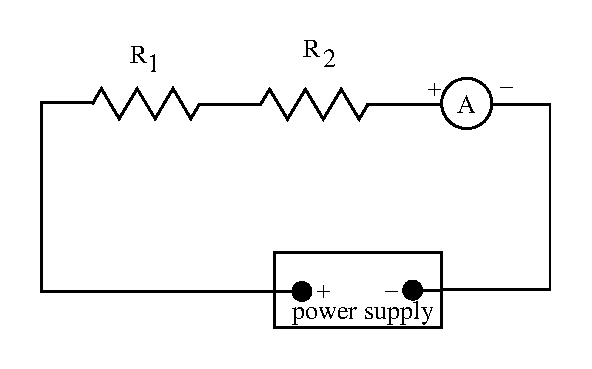
\includegraphics{ohms_law_fig_1.eps}} \par}
\vspace{0.3cm}

\begin{itemize}

\item Turn on the power supply and turn up the coarse voltage control to 
approximately 10 volts. Measure the voltages across R\( _{1} \), R\( _{2} \), 
and the milliammeter. (The voltage across the milliammeter may be in \underline{millivolts}.) Also measure the total voltage across all three elements 
in series. Record your results here:
\vspace{20mm}

\item How is the last measurement related to the three individual 
measurements?
\vspace{10mm}

\item What can you conclude about the voltage across resistors in series?
\vspace{15mm}

\item Measure the current in the series circuit and record it here:
\vspace{10mm}

%\item Connect the multimeter across both resistors, being sure to switch
%to voltage readout.
%\item When you are sure the circuit is correct, turn on the power supply
%and record the current and voltage. Turn off the power supply.\vspace{10mm}

%\item Has the current changed?\vspace{15mm}

%\item Has your previous conclusion been substantiated or refuted?\vspace{15mm}

%\item How is the voltage just measured related to the first voltage measurements
%in Activities 1 and 2?\vspace{15mm}

%\item What can you conclude about the voltage across resistors in series?\vspace{15mm}

\item Turn off the power supply.

\item Calculate R\( _{1} \), R\( _{2} \), and R\( _{A} \) from Ohm's Law and 
your above readings. Also calculate the total resistance of the circuit from 
Ohm's Law. Record your results here:
\vspace{20mm}

\item What can you conclude about the total resistance in a circuit 
containing resistors in series?\vspace{15mm}

\end{itemize}

\pagebreak

\textbf{Activity 3: Resistors in Parallel}

\begin{itemize}
\item Connect the two resistors in parallel as shown in figure \textbf{a} 
below, with the milliammeter at the point marked ``A''. Have circuit checked 
before continuing.
\end{itemize}
\vspace{0.3cm}
\begin{center}
%\includegraphics[width=6.0in]{ohms_law_fig_2.eps}
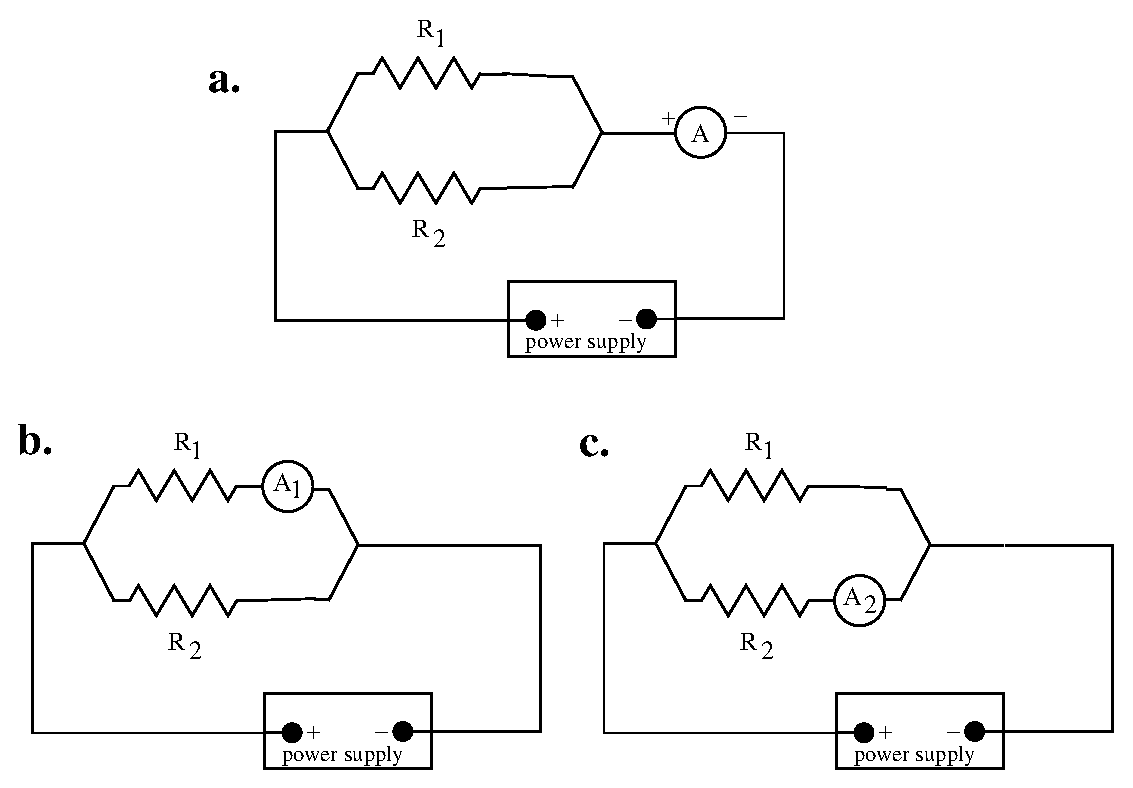
\includegraphics[width=4.6in]{ohms_law_fig_2b.eps}
\end{center}
\vspace{0.3cm}

\begin{itemize}
\item When you are sure the circuit is set up correctly, turn on the power 
supply and turn the coarse voltage control up to about 10 volts. Record the 
total current through the circuit and the voltage across 
the parallel resistance combination. Also measure the voltage across the 
milliammeter (which may be in millivolts). Turn off the power supply.
\vspace{20mm}

\item Connect the milliammeter to the point marked A\( _{1} \) in figure 
\textbf{b} above, without disturbing the rest of the circuit. Turn on the 
 power supply and 
record the current through R\( _{1} \) and the voltage across the parallel 
combination. Turn off the power supply.
\vspace{20mm}

\item Repeat the above measurements for R\( _{2} \), connecting the 
milliammeter at A\( _{2} \) as in figure \textbf{c} above. Turn off the 
power supply.
\vspace{20mm}

%\item Using Ohm's Law, calculate the two resistances of the parallel connection
%and also the total resistance of the circuit. Check with the ohmmeter
%and determine the percent differences.\vspace{30mm}

\item What is the relationship between the total current and the current
in each of the branches of the parallel circuit? (This is an example of 
Kirchhoff's junction rule which is based on conservation of charge.)
\vspace{30mm}

\item Using Ohm's Law and your data above, calculate the resistance of each 
resistor and the total resistance of the circuit.
\vspace{30mm}

\item What is the relationship between the total resistance of the parallel
circuit and the resistance of each of the branches? Look up in a reference 
what the correct relationship should be and show that your results agree 
with it.
%\vspace{15mm}

%\item Determine, using Ohm's law, what the voltage was in each branch of
%the parallel circuit. Did it make any difference that you didn't reposition
%the voltmeter during this activity? On the basis of Ohm's law, does
%the result make sense?\vspace{30mm}

%\item Can the total resistance of a series combination ever be less than
%the resistance of the largest resistor? Explain.\vspace{30mm}

%\item Can the total resistance of a parallel combination ever be greater
%than the resistance of the smallest resistor? Explain.\vspace{30mm}
\end{itemize}

 %132 equivalent

\section{Magnetism I}

Name \rule{2.0in}{0.1pt}\hfill{}Section \rule{1.0in}{0.1pt}\hfill{}Date
\rule{1.0in}{0.1pt}

\textbf{Objectives}

\begin{itemize}
\item To investigate the characteristics of magnets.
\item To understand how a compass works.
\end{itemize}
\textbf{Introduction} 

The electric interaction, you probably know, is not the only one in
which opposites attract and likes repel. Magnetic interactions have
similar characteristics. All simple magnets, regardless of size, are
bipolar: there are two magnetic poles. Consider this question, then:
Can we talk about like and unlike as we do for electricity?

\textbf{Apparatus}

\begin{itemize}
\item 2 bar magnets 
\item 2 cylindrical magnets 
\item rods and clamps
\item wool cloth
\item rubber rod
\item string
\end{itemize}
\textbf{Activity 1: The Characteristics of Magnets}

\begin{enumerate}
\item Feel the attraction between two magnets when pulled apart after having
come together without effort on your part. Describe qualitatively
in terms of strength and separation.\vspace{15mm}

\item Feel the repulsion when one of them is turned around and pushed toward
the other. Describe as in step 1.\vspace{15mm}

\item Note and describe the difference in (strength and direction of) interactions
between the ends and the middle.\vspace{15mm}

\end{enumerate}
\textbf{Activity 2: How a Compass Works}

\begin{enumerate}
\item Identify geographic north and south.
\item Hang one of the cylindrical magnets horizontally from a horizontal rod.
\item When it comes to rest, along which geographical line does the magnet
lie? \vspace{15mm}

\item Which end (colored or uncolored) is the \char`\"{}north-seeking\char`\"{}
end?\vspace{15mm}

\item Remove the cylindrical magnet and repeat step 2 with the second cylindrical magnet. Answer, again, the questions above.\vspace{15mm}

\item What happens when you bring the \char`\"{}north-seeking\char`\"{}
end of the first magnet near the hanging one's north-seeking end?\vspace{15mm}

\item What happens when you bring the first magnet's opposite end near the
second's north-seeking end?\vspace{15mm}

\item What about the first magnet's north-seeking end near the opposite
end of the hanging one?\vspace{15mm}

\item What happens when you bring the opposite ends near one another?\vspace{15mm}

\item Define in your own words like and unlike poles?\vspace{15mm}

\item What always happens between like poles?\vspace{15mm}

\item What always happens between unlike poles?\vspace{15mm}

\item Determine with a labelled bar magnet which end of your hanging magnet
should be identified as the north pole and which the south.
\vspace{10mm}
\item Why do we identify one end of a magnet as the north pole and the other
as the south?\vspace{15mm}

\item In your own words, explain a compass.\vspace{15mm}

\item In terms of magnetism, what is the earth?\vspace{15mm}

\item Charge a rubber rod with the wool cloth and bring it near the ends
of the suspended magnet; describe its effect on the magnet.\vspace{15mm}

\item Does a south magnetic pole repel a negative electric charge?\vspace{15mm}

\item Does a north magnetic pole attract a negative electric charge?\vspace{15mm}
\end{enumerate}

 %132 equivalent

\section{Magnetism II}

Name \rule{2.0in}{0.1pt}\hfill{}Section \rule{1.0in}{0.1pt}\hfill{}Date
\rule{1.0in}{0.1pt}

\textbf{Objective}

\begin{itemize}
\item To investigate the magnetic field around a permanent magnet.
\end{itemize}
\textbf{Introduction} 

The magnetic field characterizes magnetic forces in much the same way
that the electric field characterizes electric forces.
At a given point in the region around a magnet,
the strength of the field, similar to that of an electric field, is
the force per unit north pole (one positive unit of magnetism), and
the direction is indicated by the orientation of the north pole of
a compass located at the point. On earth, the field mapped out around
the magnet is actually the resultant of the field due to the magnet
and the field due to the earth.

\textbf{Apparatus}

\begin{itemize}
\item 2 bar magnets 
\item small compass 
\item white paper
\end{itemize}
\textbf{Activity 1: A Single Bar Magnet}

\vspace{0.3cm}
{\centering \resizebox*{0.45\textwidth}{!}{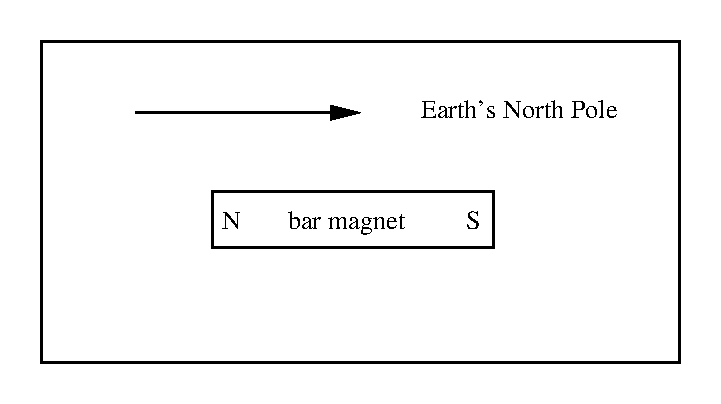
\includegraphics{magnetism_2_fig_1.eps}} \par}
\vspace{0.3cm}

\begin{enumerate}
\item Trace the outline of a bar magnet on a piece of paper. Indicate the 
magnet's polarity on the outline.
\item Place the small compass on the side of the magnet near the north pole
 and make a dot at each end of the needle using a pencil not encased in metal.
\item Move the compass forward until its south pole points at the previous
north pole dot, and make a new dot at the north pole (kind of a leap-frog 
effect).
\item Repeat 3 until the series of dots reaches the side of the magnet near 
the south pole or the edge of the paper.
\item In a similar manner, trace enough lines to map the magnetic field
over the entire paper.
%\item There are two points, called neutral points, near each end of the
%magnet where the magnet's field and the earth's field are equal and
%opposite and so cancel. At these points, the compass will align in
%no particular direction. Try to locate these points by tracing very
%carefully the lines of force in the neighborhood of the poles.
\item Do lines of force ever cross?\vspace{15mm}

\item Where is the magnetic field strongest? Weakest? How do the field
lines indicate this? Does a field line represent a constant field
along its entire length?\vspace{15mm}

\item Do the lines intersect the magnet at a particular angle (like the
electric field lines near a conductor)?\vspace{15mm}
% What does this imply about the source of a magnetic field as opposed to the 
%surface charge of a conductor as the source of an electric field? \vspace{15mm}

\end{enumerate}
\textbf{Activity 2: Two Bar Magnets--Unlike Poles Facing One Another}

\vspace{0.3cm}
{\centering \resizebox*{0.45\textwidth}{!}{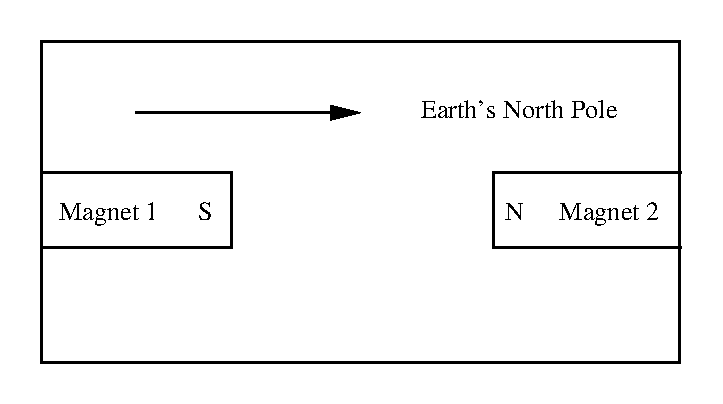
\includegraphics{magnetism_2_fig_2.eps}} \par}
\vspace{0.3cm}

\begin{enumerate}
\item Set up two bar magnets on a sheet of paper as shown in the figure
above. The magnets should be 8-10 cm apart.
\item Repeat steps 2 through 5 from the previous activity.
\item What sort of charge configuration produces an electric field that
looks similar to the magnetic field you just identified?\vspace{30mm}

\item What differences can you recognize?\vspace{30mm}

\end{enumerate}
\vspace{40mm}
\textbf{Activity 3: Two Bar Magnets--Like Poles Facing One Another}

\vspace{0.3cm}
{\centering \resizebox*{0.45\textwidth}{!}{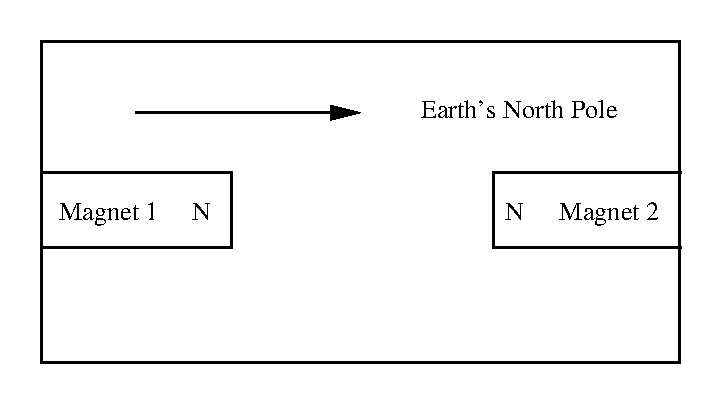
\includegraphics{magnetism_2_fig_3.eps}} \par}
\vspace{0.3cm}

\begin{enumerate}
\item Set up two bar magnets on a sheet of paper as shown in the figure
above. The magnets should be 8-10 cm apart.
\item Repeat steps 2 through 5 from Activity 1 of this investigation.
\item Try to identify on your map a point at which the magnetic field is
zero. Explain what causes this effect.\vspace{30mm}

\item What sort of electric charge configuration would produce a similar
field map?\vspace{15mm}
\end{enumerate}

 %132 equivalent

\section{Magnetism III}

Name \rule{2.0in}{0.1pt}\hfill{}Section \rule{1.0in}{0.1pt}\hfill{}Date
\rule{1.0in}{0.1pt}

\textbf{Objectives}

To investigate:

\begin{itemize}
\item The effect of magnetic fields on moving charges. 
\item The effect of moving charges (currents) on magnets. 
\end{itemize}

\textbf{Apparatus} 

\begin{itemize} 
\item Bar magnet
\item Oscilloscope
\item Tangent galvanometer
\item Compass
\item Power supply
\end{itemize}

%\textbf{Introduction} 

%Where did this intro come from??? It has nothing to do with the lab!
%A charged object moving through a magnetic field experiences a force
%which is proportional to the magnitude of its charge and to its speed
%perpendicular to the field: $F = qvB_\perp$. Changing the number of
%magnetic field lines--the flux--through a coil of wire results in
%a current in the wire. The direction of this current is such that
%the magnetic field it produces opposes the change in the external
%field. Similarly, varying the current in one coil (the primary) produces
%a current in another nearby coil (the secondary). The current in the
%second coil, too, will flow in a direction that creates a magnetic
%field opposing that which is changing in the first coil. These relationships
%between changing fields and currents are known collectively as electromagnetic
%induction.



\textbf{Activity 1: Magnetic Forces on Moving Charges }

\begin{enumerate}
\item An oscilloscope is built around the principle of the cathode ray tube. It emits electrons from its back end. These are accelerated by a series of electrodes and focused to strike a fluorescent screen at its front. The result is a visible spot (or trace) indicating voltage as a function of time.

\item \textbf{Predictions}: What, if anything, will happen to the spot on
the screen if the north pole of a magnet is brought near the left
side of the oscilloscope? What will happen if you do the same with
the south pole? What about when each of the poles are brought near
to the top? {[}Please do not touch the oscilloscope with the magnet.{]} 
\vspace{30mm}

\item Turn on the oscilloscope by pressing the power button. Turn the TIME/DIV 
knob completely counterclockwise. Adjust the INTEN (intensity) and FOCUS knobs 
so that a small bright spot is formed on the oscilloscope screen by the beam of 
electrons traveling toward the screen. Do not make the spot very bright. 
Adjust the ILLUM (illumination) knob so that the grid on the screen can be seen 
clearly. Use the horizontal and vertical POSITION controls to center the spot 
on the screen.

\item Bring the N-pole of a horizontal bar magnet near, but not touching,
the left side of the oscilloscope case at the height of the spot.
Record the direction of any deflection. Repeat with the S-pole.\vspace{20mm}

\item Bring the N-pole of a vertical bar magnet near, but not touching,
the top of the oscilloscope case just above the spot. Record the direction
of any deflection. Repeat with the S-pole.\vspace{25mm}

\item Turn off the oscilloscope.
\item Did the directions of deflections meet your expectations? Explain. 
\vspace{25mm}

\end{enumerate}

\textbf{Activity 2: The Effect of Moving Charges (Currents) on Magnets}

In this investigation we will use a device known as a tangent galvanometer to make a qualitative study of the effect of current (moving charges) in a coil of wire on a compass. A sketch of the galvanometer is shown below.

\begin{center}
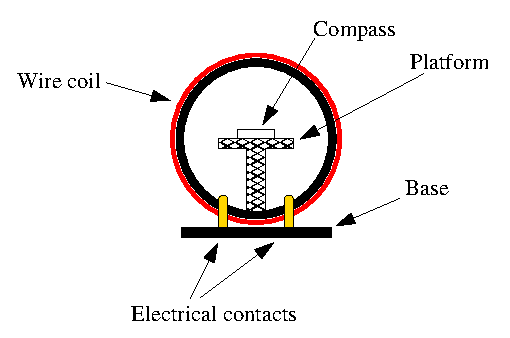
\includegraphics{tangent_galvanometer.eps}
\par
Figure 1. Tangent galvanometer and compass.
\end{center}

\begin{enumerate}

\item With the power supply off, connect the positive and negative terminals 
on the power supply to the two side screws on the tangent galvanometer. Turn 
the coarse current control on the power supply all the way up and the voltage 
controls all the way down.

\item Before turning the power supply on, place the compass on the platform 
in the center of the tangent galvanometer. Rotate the galvanometer until the 
compass needle is aligned with the plane of the wire coil of the galvanometer.
Turn the power supply on and slowly turn up the \underline{fine} voltage 
control. What do you observe? Make a sketch to show the orientation of the 
compass needle and galvanometer coil with the voltage on and off. 
(It may be easiest to do this with TOP views.)
\vspace{20mm}

\newpage

\item Turn the voltage on the power supply to zero.
Rotate the entire setup (galvanometer, compass, wires) $180^\circ$
so the contacts are on the opposite side from where they were before.
Make sure the compass needle is again aligned with the plane of the wire coil.
Slowly turn the voltage back up. What do you observe?
Make another sketch to show the orientation of the compass needle and
galvanometer coil with the voltage on and off.
\vspace{30mm}

\item The deflection of the compass when current flows in the tangent 
galvanometer implies the current creates a magnetic field.
From your observations can you tell the direction
of the magnetic field?  Explain.
\vspace{30mm}

\item Reverse the wires on the contacts of the tangent galvanometer to reverse 
the direction of the current in the coil of the galvanometer.
We will now repeat the observations from above.
With the voltage off, align the compass needle and the plane of the wire coil 
of the galvanometer as in number 2 above.
Slowly turn up the voltage.
What do you observe?
Make a sketch to show the orientation of the compass and
galvanometer coil with the voltage on and off.
\vspace{30mm}

\item Rotate the entire setup (galvanometer, compass, wires) $180^\circ$
so the contacts are on the opposite side from where they were before.
Make sure the compass needle is again aligned with the plane of the wire coil.
Slowly turn the voltage back up. What do you observe?
 Make another sketch.
\vspace{30mm}

\item Based on your observations, what happens to the magnetic field of the 
tangent galvanometer when you reverse the direction of the current?

\end{enumerate}
 %132 equivalent
\setcounter{equation}{0}

\section{Magnetic Field of the Earth}

Name \rule{2.0in}{0.1pt}\hfill{}Section \rule{1.0in}{0.1pt}\hfill{}Date
\rule{1.0in}{0.1pt} 

\textbf{Objective}

\begin{itemize}
\item A measurement of the earth's magnetic field.
\end{itemize}
\textbf{Introduction} 

The magnetic field lines of a bar magnet, though emanating from its
full length, are densest near the poles. These lines are typically
not perpendicular to the faces of the magnet. The Earth, as you know,
is like a giant bar magnet, with its magnetic south pole near its
geographic north pole.

The field lines of the Earth's magnetic field, therefore, tend to
point obliquely at any given spot on its surface. The angle (let's
call it \( \phi  \)) that a line makes with a surface is known as
its \emph{dip angle} (see figure). Thus, each locality on earth has
its characteristic value for \( \phi  \) with regard to the terrestrial
magnetic field.

\begin{center} \begin{picture}(200,70) \put(0,0){\line(1,0){200}} \put(150,50){\vector(-2,-1){100}} \put(150,50){\vector(0,-1){50}} \put(150,50){\vector(-1,0){100}} \put(100,60){\makebox(0,0){$B_h$}} \put(160,25){\makebox(0,0){$B_v$}} \put(90,30){\makebox(0,0){$\bf B$}} \put(75,6){\makebox(0,0){$\phi$}} \put(60,0){\oval(10,10)[tr]} \end{picture} \end{center}

The horizontal component of the Earth's magnetic field,

\begin{equation}
B_h = B\cos\phi,
\end{equation}

causes the magnetized needle of a compass to align in the geographic
north-south direction.

%%This is about 1000 times more complicated than it has to be!
% by producing a torque on it. Recall that the
%magnitude of a torque is \( \tau  \) = r F\( \sin \theta  \), where
%F is the force, r is the distance from the axis of rotation to the
%point at which the force acts, and \( \theta  \) is the angle between
%the line from the axis of rotation to the point of interaction and
%the direction of the force.
%
%\begin{center} \begin{picture}(200,75) \put(0,0){\line(0,1){10}} \put(150,0){\line(0,1){10}} \put(65,5){\vector(-1,0){65}} \put(85,5){\vector(1,0){65}} \put(75,5){\makebox(0,0){$\bf r$}} \put(0,15){\circle*{3}} \put(80,55){\makebox(0,0){$\tau = r F \sin\theta$}} \put(150,15){\vector(0,1){50}} \put(150,15){\vector(3,4){37.5}} \put(160,20){\makebox(0,0){$\theta$}} \put(130,35){\makebox(0,0){$F \sin\theta$}} \put(170,50){\makebox(0,0){$\bf F$}} \thicklines \put(0,15){\line(1,0){200}} \end{picture} \end{center}
%
%The force on the compass is due to the Earth's magnetic field,
%F = pB, where p is the so-called \emph{pole strength} (recall that
%F = qE, for static electric fields, where q is the charge). In this
%case, the force acts on both ends of the magnet, so that r (the distance
%from the axis of rotation to the point at which the force acts) is
%half the length of the compass needle, $l$; \( \theta  \) is the
%angle between the alignment of the compass needle and the direction
%of B\( _{h} \). Hence, the torque on a compass needle due to the
%Earth's magnetic field is
%
%\begin{displaymath} \tau_e = plB_h\sin\theta. \end{displaymath}
%

You will use a tangent galvanometer to produce an additional horizontal
magnetic
field perpendicular to the Earth's field (in other words, one that
points east or west).
A tangent galvanometer consists of a vertical, circular coil of wire
with N turns, a pedestal compass at the center of the coil, and electrical
contacts so that a direct current can be established in the coil.
The magnetic field at the center of the galvanometer coil caused by a current
I in the coil is

\begin{equation}
B_c = N\frac{\mu_0I}{2R}
\end{equation}

where R is the radius of the coil and \( \mu _{0} \) is the permeability
of free space (1.25664 x 10\( ^{-6} \) T\( \cdot  \)m/A). B\( _{c} \)
is perpendicular to the vertical plane of the coil. If the plane of
the coil is placed in the north-south direction (that is, parallel
to the compass needle when there is no current in the coil), then,
when there is current in the coil, the compass will be influenced
by two perpendicular fields, B\( _{h} \) and B\( _{c} \). 
The compass needle will now point in the direction of the vector
sum ${\bf B}_h+{\bf B}_c$.  

Let $\theta$ be the angle through which the compass needle turns
when the current in the tangent galvanometer is turned on.
In other words, $\theta$ is the angle between ${\bf B}_h$ and
${\bf B}_h+{\bf B}_c$.  Sketch a picture of these vectors, and
use it to convince yourself that

%The
%latter provides a second torque (see figure, checking carefully the
%angles, \( \cos \theta =\sin (\frac{\pi }{2}-\theta ) \) ):
%
%\begin{displaymath} \tau_c = plB_c\cos\theta \end{displaymath}
%
%\begin{center} \begin{picture}(150,150) \put(10,75){\line(1,0){100}} \put(60,25){\line(0,1){100}} \put(5,75){\makebox(0,0){W}} \put(60,130){\makebox(0,0){N}} \put(115,75){\makebox(0,0){E}} \put(60,20){\makebox(0,0){S}} \put(34,40){\vector(3,4){54}} \put(34,40){\vector(-1,0){10}} \put(34,40){\vector(0,-1){10}} \put(88,112){\vector(1,0){10}} \put(88,112){\vector(0,1){10}} \put(65,90){\makebox(0,0){$\theta$}} \multiput(34,40)(12,-9){4}{\line(4,-3){10}} \multiput(88,112)(12,-9){4}{\line(4,-3){10}} \multiput(60,75)(12,-9){2}{\line(4,-3){10}} \put(15,40){\makebox(0,0){$\scriptstyle pB_c$}} \put(108,112){\makebox(0,0){$\scriptstyle pB_c$}} \put(34,25){\makebox(0,0){$\scriptstyle pB_h$}} \put(88,127){\makebox(0,0){$\scriptstyle pB_h$}} \put(92,81){\makebox(0,0){$\scriptstyle r$}} \put(104.5,43){\makebox(0,0){$\scriptstyle l$}} \put(89,77){\vector(-3,-4){10}} \put(95,85){\vector(3,4){10}} \put(100,37){\vector(-3,-4){20}} \put(109,49){\vector(3,4){20}} \end{picture} \end{center}
%
%When current is established in the coil, the needle will rotate through
%an angle \( \theta  \) with respect to the plane of the coil until
%the opposing torques are equal in magnitude. Thus, when equilibrium
%is established, we have
%
%\begin{displaymath} \tau_e = \tau_c \Rightarrow plB_h\sin\theta = plB_c\cos\theta \end{displaymath}

\begin{equation}
%\begin{displaymath} 
B_h = \frac{B_c}{\tan\theta} 
%\end{displaymath}
\end{equation}

\vskip 1in

By measuring the angle $\theta$, we can determine $B_h$.  
If we then measure the dip angle $\phi$, we can determine
the Earth's magnetic field from equation (1) above.

\textbf{Apparatus}

\begin{itemize}
\item tangent galvanometer 
\item power supply 
\item DC ammeter (0-1 amp)
\item banana plug leads (1 red, 2 black) with alligator clips
%\item switch
\item compass
\item ruler 
\item dip angle compass 
%\item wooden stand
\end{itemize}
\vspace{15mm}
\textbf{Activity}

\begin{enumerate}
\item Measure and record on the accompanying data sheet the diameter D of
the galvanometer coil. Calculate and record the radius R of the coil.
\item Count and record the number of turns, N, of the coil.
\item With the power supply off, connect its positive and negative terminals 
to the tangent galvanometer and  a DC ammeter (in series). 
Be sure the ammeter is connected in \underline{series} with 
the coil. Use long wires to connect the outside terminals of the coil
to the circuit so that the coil may be removed from the magnetic effects
of the ammeter and power supply. Be sure no magnetic material other
than the compass is in the vicinity of the coil. Turn the coarse current 
control on the power supply all the way up and the voltage controls all the 
way down.
\item Place the compass on the platform of the tangent galvanometer and rotate  
the galvanometer until the compass needle is aligned with the plane of the wire 
coil of the galvanometer. Rotate the compass body so that the needle points 
north and south on the compass.
\item Turn on the power supply and slowly turn up the fine voltage control 
until the current is about 0.2 A as measured with the orange ammeter.
Note that the compass needle rotates. It might be a good idea to tap
lightly the face of the compass to be sure the needle hasn't become
stuck. Record the current and the displacement angles at both the
north and south poles of the needle. Calculate B\( _{c} \) from equation (2).
\item Average the north and south angles; use this average to calculate 
B\( _{h} \) from equation (3).
\item Repeat steps 5 and 6 for currents of 0.4 A, 0.6 A, and 0.8 A.
\item Reverse the current (by switching the two leads at the galvanometer coil)
 and repeat steps 5, 6 and 7.
\item Determine and record the dip angle at two separate locations in the 
classroom (using the dip angle compasses). Average these measurements and use 
the result for the dip angle, \( \phi  \).
\item Using equation (1) above, calculate the Earth's magnetic field 
\textbf{B} for each set of data. Remember that in equation (1), \( \phi  \) 
is the \underline{dip angle}, not the displacement angle of the compass.
Calculate an average value for \textbf{B} and a standard deviation.
How far off, in terms of numbers of standard deviations, is your result
from the accepted value for Richmond, $5.1 \times 10^{-5}$ T?
\end{enumerate}
\hrulefill

\newpage

{\centering \textbf{Data Sheet}\par}

%Diameter of Coil, D (m) \> \rule{2cm}{.1pt}  

Diameter of Coil, D (m)  \rule{2cm}{.1pt}  

Radius of Coil, R (m) \rule{2cm}{.1pt} 

Number of Turns of Coil, N  \rule{2cm}{.1pt}

Dip Angle, \( \phi  \) (\( ^{\circ } \)): reading 1 \rule{1cm}{.1pt}
~~reading 2 \rule{1cm}{.1pt}

Average Dip Angle, \( \phi  \) (\( ^{\circ } \)): \rule{2cm}{.1pt}

\vspace{0.3cm}
{\centering \begin{tabular}{|c|c|c|c|c|c|c|}
\hline 
Current  &
Coil Field &
North Angle &
South Angle &
Average Angle &
Horizontal &
Earth's Field \textbf{B} \\
(A)&
B\( _{c} \) (T)&
\( \theta  \)\( _{N} \) (\( ^{\circ } \))&
\( \theta  \)\( _{S} \) (\( ^{\circ } \))&
(\( ^{\circ } \))&
Component B\( _{h} \) (T)&
(T)\\
\hline 
&
&
&
&
&
&
\\
\hline 
&
&
&
&
&
&
\\
\hline 
&
&
&
&
&
&
\\
\hline 
&
&
&
&
&
&
\\
\hline 
&
&
&
&
&
&
\\
\hline 
&
&
&
&
&
&
\\
\hline 
&
&
&
&
&
&
\\
\hline 
&
&
&
&
&
&
\\
\hline
\end{tabular}\par}
\vspace{0.3cm}

\vspace{15mm}
Earth's Magnetic Field (measured), <\textbf{B}> (T) \rule{2cm}{.1pt}

Standard Deviation on Measurement, \( \sigma _{B} \) (T) \rule{2cm}{.1pt}

Number of Standard Deviations from Accepted Value, \( \frac{\left| <B>-B_{accepted}\right| }{\sigma _{B}} \):
\rule{2cm}{.1pt} 

\textbf{Show calculations for one trial here:}
 %132 equivalent
\setcounter{equation}{0}
\setcounter{figure}{0}

\section{Electromagnetic Induction}

Name \rule{2.0in}{0.1pt}\hfill{}Section \rule{1.0in}{0.1pt}\hfill{}Date
\rule{1.0in}{0.1pt}

\textbf{Objectives}

To investigate:

\begin{itemize}
\item The effect of changing magnetic fields on induced emf and current.
\end{itemize}
\textbf{Introduction} 

%A charged object moving through a magnetic field experiences a force
%which is proportional to the magnitude of its charge and to its speed
%perpendicular to the field: $F = qvB_\perp$. 
If the magnetic flux through a coil of wire changes, an emf (or voltage) 
will be induced in the coil. This is Faraday's Law. If the coil of wire 
forms a closed loop, then a current will be induced in the wire. The direction 
of this current is such that the magnetic field it produces opposes the change 
in the external field. This is known as Lenz's Law. Similarly, varying the 
current in one coil (the primary) produces a current in another nearby coil 
(the secondary) due to the varying magnetic field produced by the first coil. 
The current in the second coil, too, will flow in a direction that creates a 
magnetic field which opposes the change in the field of the first coil (again, 
due to Lenz's Law). 
These relationships between changing fields and currents are known 
collectively as electromagnetic induction.

\textbf{Apparatus} 

\begin{itemize}
\item one small wire coil
\item voltage sensor
\item two alligator clips
\item bar magnet
\item Pasco 750 Interface
\end{itemize}

\textbf{Activity: A Moving Magnet and a Coil}

\begin{enumerate}
\item Connect the coil to the voltage sensor using the alligator clips. Connect the voltage sensor to port A on the Pasco 750 interface.
\item Turn on the computer and launch {\it EM Induction} in the $132 Workshop$ 
under $Physics Applications$ in the {\bf Start, Programs} menu.

\item Place a bar magnet vertically along the axis of the small coil with
the N-pole touching the coil.

\item Start recording data and lift the bar magnet quickly straight up.

\item At the end of the data taking interval, the computer should display
a value for the electromotive force (emf) induced in the small coil.
Several trials may be required to get the correct timing between starting
the data acquisition and removing the magnet. Note and record the sign of the 
induced emf.\vspace{10mm}

\item \textbf{Prediction}: If you lower the magnet, N-pole down, quickly
toward the coil, what will be the sign of the emf? \vspace{15mm}

\item Carry out the experiment, starting the data acquisition, then lowering the magnet.
Record the sign of the induced emf.\vspace{10mm}

\item Did your result confirm or refute your prediction?\vspace{20mm}

\item \textbf{Prediction}: What will happen to the emf if you perform the
same pair of experiments with the S-pole toward the coil? \vspace{20mm}

\item Perform the two experiments, lifting and lowering the magnet, with
the S-pole down. Record the sign of the induced emf in each case.\vspace{20mm}

\item How did the results compare with your predictions?

\end{enumerate}
 %132 equivalent

\section{Electromagnetic Induction II}

Name \rule{2.0in}{0.1pt}\hfill{}Section \rule{1.0in}{0.1pt}\hfill{}Date
\rule{1.0in}{0.1pt}

\bigskip
\bigskip
\bigskip


\textbf{Introduction}.
In this lab, we'll take a further look at Faraday's Law, which says
that a changing magnetic field can produce an emf (that is, a voltage)
in a loop of wire.  Current will be supplied to a large coil (which is a 
series of loops of wire), resulting in a magnetic field.  
If the current were constant in time,
then a steady magnetic field would be produced.  Since we want to
produce a changing magnetic field, we supply the coil with {\it
alternating current}, that is, current that flows back and forth in
alternating directions, oscillating in a sine-wave fashion.  The
result is an ever-changing magnetic field, which induces an emf in
a separate small coil.

\textbf{Apparatus}

\begin{itemize}

\item one large wire coil

\item one small wire coil

\item two banana plug leads with alligator clips

\item voltage sensor

\item Pasco 750 Interface

\end{itemize}

{\bf Setup.} The apparatus should be wired up to the computer interface in the 
following way: The two ends of the large coil should be connected to the output
terminals on the right side of the interface (using the banana plug leads with 
alligator clips). These output terminals supply alternating current to the 
large coil. The two ends of the small coil should be connected to a voltage 
sensor, which is plugged into port A on the interface. Place the small coil in 
the center of the large coil. Both coils should be arranged horizontally (that 
is, with the axes pointing straight up and down). If you are not sure whether 
things are hooked up correctly, consult your instructor.

{\bf Activity 1: Qualitative predictions.} Suppose that the top graph on the 
last page of this experiment represents the current flowing through the large 
coil as a function of time. When $I$ is positive, that means current is 
flowing in one direction around the coil, and when $I$ is negative the current 
is flowing in the other direction. On the axes below the top graph, sketch the 
shapes of the following other quantities.
In each case, don't worry about the overall scale on the vertical axis;
just focus on the shapes of the graphs, and particularly the locations
of the peaks and valleys.  Hint: some of the graphs will be exactly
the same shape as the given graph of $I$.

\begin{enumerate}
\item
On the first set of axes, sketch the vertical component of the magnetic field,
$B_z$, at the center of the large coil (realizing that this field is directly
proportional to the current in the coil).
\item On the the next set of axes, sketch the magnetic flux $\Phi_ B$ passing
through the small coil. (This flux is proportional to the magnetic field 
produced in the large coil).
\item On the bottom set of axes, sketch the emf ${\cal E}$ induced in the small
coil (which, by Farady's law, is proportional to the negative time derivative 
of the flux through the coil).
\end{enumerate}

The computer will measure and graph
$I(t)$, the current in the large coil, and ${\cal E}(t)$,
the emf in the small coil.  We want to test whether the two graphs are related
to each other in the way you predicted.  To be specific, make the following
predictions from your graphs before trying the experiment:

\newpage

\begin{enumerate}
\item At times when $I(t)$ is at its maximum value, what is ${\cal E}$?
\vskip .8in
\item At times when $I(t)$ is at its minimum value, what is ${\cal E}$?
\vskip .8in
\item At times when $I(t)=0$, what is ${\cal E}$?
\vskip .8in
\end{enumerate}

\bigskip\bigskip

{\bf Activity 2: Testing the predictions.}

Start the program called ``induction2.'' You should see two graphs,
one showing the current in the large coil and one showing the emf (voltage)
across the small coil.  Both graphs will be blank until you start taking
data, of course.  There should be an additional box that allows you to control
the frequency of oscillation of the alternating current.  Leave this alone
for now; we'll mess around with it later.

Hit ``Start'' and take data for about 5 seconds.  Do the shapes of the
two graphs generally match your predictions from Activity 1? (To answer this, you may want to expand the scales of the horizontal axes of the graphs so you can see the shapes better, and also align the graphs so that the times are synchronized.) 

\vskip 1in

If the answer to this question is ``yes,'' then go on.  If it's ``no,
the shape of the second one is exactly the opposite of what I expected,''
then you just have the small coil upside-down.  Turn it over and 
try again.  If the answer is not one of those two, then consult your 
instructor.

Let's be a bit more specific in comparing the predictions
with the data.  Examine the current graph, and record the
times of the first four moments when the current reaches a maximum.
Then look at the other graph, and record the emf at those same four times.
Are the results consistent with your prediction number 1 in Activity 1?

\newpage

Perform a similar analysis to check your predictions 2 and 3 from Activity 1.
In each case, check several appropriately-chosen moments of time to see
if the relationship between $I$ and ${\cal E}$ is as you predicted.

\vskip 4in

Suppose that you rotate the small coil 90$^\circ$, so that its axis
is horizontal.  What do you predict about the resulting emf?
Test your prediction and record the results here.

\newpage

\begin{center}

{\bf Graphs for Activity 1}

\vfil

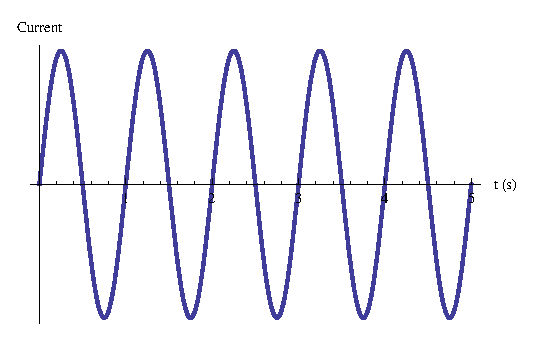
\includegraphics[width=2.9in]{indfig1.eps}

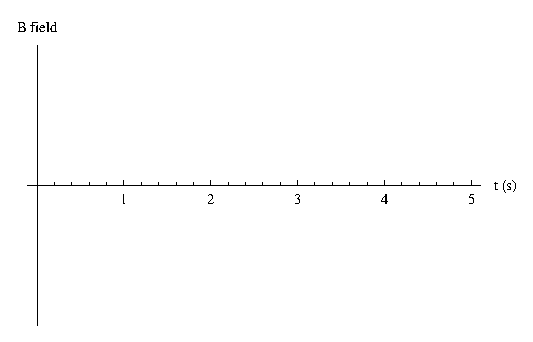
\includegraphics[width=2.9in]{indfig2.eps}

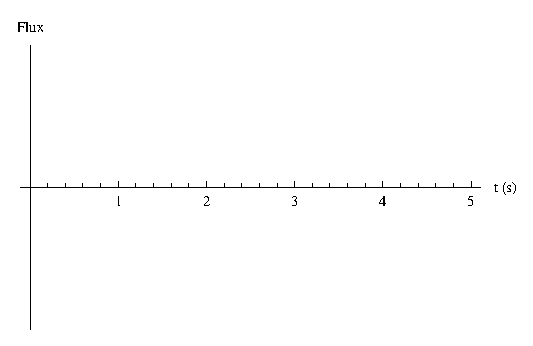
\includegraphics[width=2.9in]{indfig3.eps}

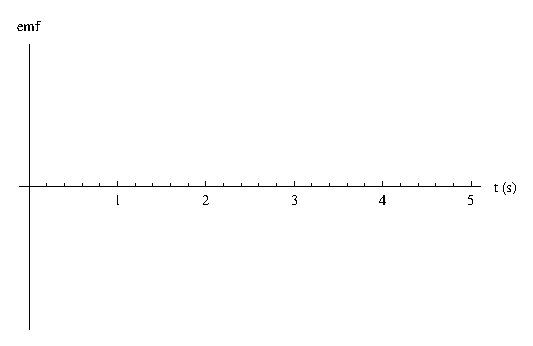
\includegraphics[width=2.9in]{indfig4.eps}



\vfil

\end{center}


 %132 equivalent

%--------------------------------------------
\part{Optics}


\section{Refraction of Light}

Name \rule{2.0in}{0.1pt}\hfill{}Section \rule{1.0in}{0.1pt}\hfill{}Date
\rule{1.0in}{0.1pt}

\textbf{Objective}

To investigate the path traveled by light through a plate of plexiglass
(a transparent solid material).

\textbf{Introduction}

The speed of light depends on the medium in which it travels. In passing
from one medium, at least some light energy is reflected. If the second
medium is transparent, most of the light will pass into and through
it. If the beam is not perpendicular to the boundary between the two
media, it will bend as it enters, an effect known as refraction. The
direction a single ray of light travels when refracted is given by
Snell's law:

\begin{displaymath} \frac{sin~i}{sin~r} = \frac{v_1}{v_2} = \frac{n_2}{n_1} \end{displaymath}

where

\begin{quote}
i = incident angle

r = refracted angle

v\( _{1} \) = light speed in medium 1

v\( _{2} \) = light speed in medium 2

n\( _{1} \) = index of refraction of medium 1 

n\( _{2} \) = index of refraction of medium 2
\end{quote}
\textbf{Note}: All angles are measured from the normal to the boundary
at the point the ray enters the medium. The index of refraction is
the ratio of light's speed in a vacuum, $c$, to its speed in the medium,
$v$: $n = c / v$. It is worth remembering that $n_{air} \approx 1.00$.

\vspace{0.3cm}
{\centering 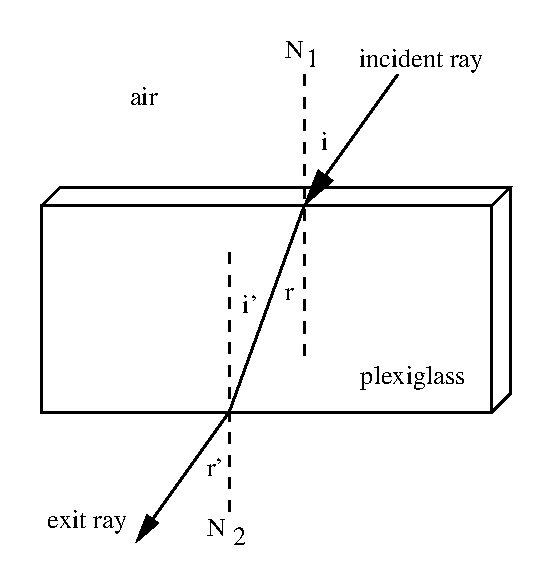
\includegraphics{refraction_of_light_fig_1.eps} \par}
\vspace{0.3cm}

\vspace{15mm}
\textbf{Apparatus} 

\begin{itemize}
\item light fence 
\item plexiglass block 
\item white paper, pins, and wood board 
\item protractor
\end{itemize}
\textbf{Activity} 

\begin{enumerate}
\item Put a plexiglass plate at the center of a piece of paper. Outline
its position. Identify a normal, $N_1$, perpendicular to an edge of
the plate.
\item Arrange the light source apparatus so that the parallel rays of light
cross the paper and are incident at a $30^\circ$-$35^\circ$ angle
to the normal. Trace one of these rays.
\item Sight the corresponding ray as it emerges from the other side of the
plexiglass. Trace this ray.
\item Remove the plexiglass and connect the points where the light ray entered 
and left the plexiglass with a straight line. This represents the path of the 
light ray as it passes through the plexiglass.
\item Construct the normal, $N_2$, and measure and record $i$, $r$, $i'$, and 
$r'$.
\vspace{20mm}

\item Repeat the above procedure for two more incident angles between
$40^\circ$ and $60^\circ$.
\vspace{30mm}

\item Plot a graph of $sini$ as a function of $sinr$, including the point (0,0)
 which corresponds to a light ray incident perpendicular to the plexiglass. 
Include a linear trendline and don't forget to include a title and axis labels. 
Print the graph and include it with this unit.

\item Determine the slope of the graph, $n_{plexiglass}$, based on your data. Do 
not include more than three significant fugures.
\vspace{20mm}

\item Does $i = i'$? Explain.
\vspace{20mm}

\item Does $r = r'$? Explain.
\vspace{20mm}

\item Are the incident and exit rays parallel? Explain.
\vspace{20mm}

\item What is the speed of light in the plexiglass?
\vspace{20mm}

\item Under what conditions would a refraction angle be greater than an
incident angle?
\vspace{20mm}

\item Collect the results from the other lab groups and determine an average 
and standard deviation for the index of refraction of the plexiglass.
\end{enumerate}

 %132 equivalent

\section{Refraction at Spherical Surfaces: Thin Lenses}

Name \rule{2.0in}{0.1pt}\hfill{}Section \rule{1.0in}{0.1pt}\hfill{}Date
\rule{1.0in}{0.1pt}

\textbf{Objective}

\begin{itemize}
\item To investigate thin lenses.
\end{itemize}
\textbf{Introduction} 

A lens converges or diverges light rays. It is a transparent material
bounded, in the case of thin lenses, by spherical edges. The line
between the centers of curvature of these edges is referred to as
the principal axis. The principal focus is the point on the principal
axis where parallel incident rays converge. The distance from the
lens to this point is known as the focal length. The relation between
the focal distance, $f$, the object distance, $p$, and the image distance,
$q$, is:

\begin{displaymath} \frac{1}{p} + \frac{1}{q} = \frac{1}{f}. \end{displaymath}

\textbf{Apparatus}

\begin{itemize}
\item light fence
\item converging (convex) lens in holder
\item converging and diverging lenses (1 each) without holders
\item optical bench 
\item light source with 12v output power source
\item optical viewing screen (white)
\item plastic ruler
\end{itemize}
%\textbf{Investigation 1: The Converging Lens}

\textbf{Activity 1}

\begin{itemize}
\item Arrange the light source apparatus so that the parallel rays of light
cross a piece of paper. 
\item Place a convex lens (without holder) on the paper perpendicular to the 
central ray.
Outline its position and the path of the rays. Pay particular attention
to the condition near the principal focus.
\item What is the focal length of this lens?\vspace{15mm}
\item Include a sketch of the light rays in your lab book, showing the focal point and focal length of the lens.
\end{itemize}
\textbf{Activity 2 }

\begin{itemize}
\item Place the light source in its bracket at one end of the optical bench. The arrow on the light source will be the object in this investigation. Measure
and record its height, $h_0$.\vspace{10mm}

\item Place a converging lens in its holder on the optical bench 70 cm from the object (this is the object distance $p$). Turn on the light source and position the optical viewing screen on the optical bench so that a sharp image of the arrow appears on the screen. Measure the distance of the screen from the lens. This is the image distance $q$. Also measure the height of the image $h_i$. Record $p$, $q$, and $h_i$ in the first line of the following table.
\end{itemize}
\vspace{0.3cm}
{\centering \begin{tabular}{|c|c|c|c|c|c|}
\hline 
~~~~~~~\( p \)~~~~~~~&
~~~~~~~\( q \)~~~~~~~&
~~~~~~~\( h_{i} \)~~~~~~~&
~~~~~~~\( \frac{h_{i}}{h_{0}} \)~~~~~~~&
~~~~~~~\( \frac{q}{p} \)~~~~~~~&
~~~~~~~\( f \)~~~~~~~\\
\hline
\hline 
&
&
&
&
&
\\
\hline 
&
&
&
&
&
\\
\hline 
&
&
&
&
&
\\
\hline 
&
&
&
&
&
\\
\hline 
&
&
&
&
&
\\
\hline
\end{tabular}\par}
\vspace{0.3cm}

\begin{itemize}
\item Move the lens to create four more object distances of 60, 50, 40, and 30 cm. In each case, measure the image distance and the height of the image and record in the above table. Calculate and record the ratios of the image and object heights, $h_i / h_0$, and the image and object distances, $q / p$. Record these values in the above table. You should now have the first five columns of the above table filled in.
\item Calculate and record the focal length, $f$, for each observation. Show one of the calculations here:\vspace{15mm}
\item Determine an average focal length, $f_{ave}$, and a standard deviation based on your five values.
\vspace{15mm}
\item What is the relationship between the ratio of the image to object
heights and the ratio of image and object distances? The first ratio
is called the magnification.\vspace{15mm}

\item Replace the converging lens with a diverging one. Try to obtain a
real image on a piece of white paper.
\item Why can you not form a real image with a diverging lens?\vspace{15mm}

\end{itemize}
%\textbf{Investigation 2: Lenses in Combination (Optional)}

%\textbf{Activity}

%\begin{itemize}
%\item Place a converging lens and a diverging lens together into the lens
%holder. Check to see that you can get a real image with this combination.
%\end{itemize}
%\vspace{0.3cm}

%\begin{itemize}
%\item Repeat the five sets of observations of Investigation 1, Activity
%2, to get an equivalent focal length $f_{ave}^{eq}$.\vspace{40mm}

%\end{itemize}
%\textbf{Investigation 3: The Diverging Lens}

%\textbf{Activity 1 (Optional)}

%\begin{itemize}
%\item Using the relation:
%\end{itemize}
%\begin{displaymath} \frac{1}{f^{eq}} = \frac{1}{f_1} + \frac{1}{f_2}, \end{displaymath}

%\begin{quote}
%determine the focal length of the diverging lens, $f_2$. Use $f^{eq}_{ave}$
%for $f^{eq}$ and $f_{ave}$ for $f_1$.\vspace{2in}

%\end{quote}
\textbf{Activity 3}

\begin{itemize}
\item Repeat the procedure of Activity 1 with a concave lens. Locate the 
principal focus by extending the refracted rays backwards.

\item What is the focal length of this lens?
\vspace{15mm}

\item Include a sketch of the light rays in your lab book, showing the focal 
point and focal length of the lens.
\end{itemize}

 %132 equivalent

\section{The Interference of Light}

Name \rule{2.0in}{0.1pt}\hfill{}Section \rule{1.0in}{0.1pt}\hfill{}Date
\rule{1.0in}{0.1pt}

\textbf{Objective}

\begin{itemize}
\item To investigate the interference of light waves as they pass through
a set of slits. 
\end{itemize}
\textbf{Apparatus}

\begin{itemize}
\item Basic optics diode laser
\item Optical bench with rotary motion sensor
\item Phototransistor for measuring light intensity (mounted on rotary motion sensor)
\item ``Multiple Slit Set'' slit accessory
\item Glass plate with sets of narrow slits
\item {\it DataStudio} 750 Interface
\end{itemize}
\textbf{Introduction}

In this laboratory you will investigate the interference of light
produced by a laser beam passing through a set of narrow, adjacent
slits. When light passes the slits each opening acts as an independent
source of waves that can overlap one another to produce a distinctive
pattern of bright and dark spots on a screen. The position of the
bright spots depends on the separation of the adjacent slits and the
wavelength of the incident light. 

You can measure this interference pattern with the setup shown below. 
(This is a \underline{top} view of the set-up.) 
A phototransistor is seated behind the narrow opening on top of the large,
metal mount sitting on a rail. The phototransistor can translate the intensity 
of the light falling on it into a voltage signal that can be read by the
computer. In addition, the phototransistor can be moved back and
forth on a rotary motion sensor that measures the position of the 
mount. These two signals can be combined to
make a graph of the intensity as a function of position.

\vspace{0.3cm}
%{\centering \resizebox*{0.75\textwidth}{!}{\includegraphics{interference_of_light_fig_1.eps}} \par}
{\centering \resizebox*{0.75\textwidth}{!}{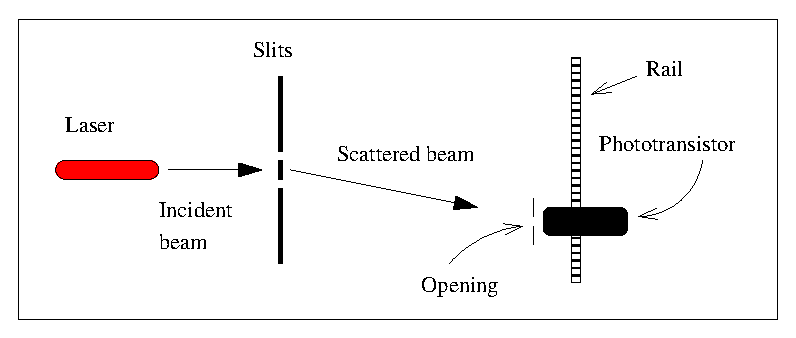
\includegraphics{interference_of_light_fig1b.eps}} \par}
\vspace{0.3cm}

In this unit you will pass light from the laser through slits of known
separation and use the interference pattern to determine the wavelength
of the light.

\textbf{Activity 1: An Alternative View}

Isaac Newton believed that light was made up of small, unseen particles
that obeyed (surprisingly enough!) Newton's Laws. This view is known
as the corpuscular theory. We want to consider how this model of light
predicts different behavior from the wave theory.

\vspace{35mm}
(a) Consider a laser beam shining on a circular hole. If a beam of
light consisted of small, unseen particles that behaved as tiny billiard
balls what would you see on a screen that is downstream from the circular
hole? A sketch might be useful here.
\vspace{30mm}

(b) Now consider the same laser beam shining on a pair of narrow slits.
What would you see on a screen downstream from the slits if light
were made of corpuscles?
\vspace{30mm}

For the questions above you should have predicted that the laser would
form a single bright spot (for part a) or two parallel lines (for part
b). The experiment you are about to perform provided compelling evidence
that Newton's corpuscular theory was wrong. 

\textbf{Activity 2: The Interference of Light }

(a) You are now ready to turn on the laser. DO NOT LOOK DIRECTLY INTO
THE BEAM OR POINT THE LASER CARELESSLY ABOUT THE ROOM. Mount the laser on the 
optical bench at the opposite end from the rotary motion sensor. Turn on the
laser and you should see the bright red spot of the beam striking
the rotary motion sensor assembly. On the ``Multiple Slit Set'' accessory, 
select a double slit of width .04 mm amd separation .125 mm. Rotate the 
wheel so that the double slit is at the center of the opening.
%You should have a glass plate with a green border and several
%different slit arrangements on it. Place the opening in the center
%of the plate in the path of the laser beam. The adjacent slits in
%the center hole are 0.03295 mm apart. What do you see? 
\vspace{10mm}

%(b) Position the glass plate about 30-40 cm from the phototransistor
%mount with the central maximum (the brightest spot) 
%striking the center hole. Measure and record this
%distance. You may find it useful to use the plumb line to measure
%this distance.
(b) Position the double slit about 70 cm from the phototransistor mount. Adjust 
the laser beam direction so that it falls on the double slit you have selected. 
(There are two adjustment screws on the back of the laser.) 
You should see the interference pattern on the phototransistor mount. 
\vspace{10mm}

(c) Position the phototransistor mount so the interference pattern
is at the same height as the opening in the center of the phototransistor mount. The phototransistor is mounted behind this hole. To make accurate measurements it is important to carefully determine the geometry of your setup. Check to see if the slits and the phototransistor mount are perpendicular to the incident
laser beam.  You want to make sure the phototransistor can {}``see'' as many
bright spots as possible. Carefully slide the phototransistor mount back and forth to make sure that it stays centered on the interference pattern. Then set it 
at one side of the pattern to begin the experiment.
Start the ``Interference'' activity in the {\bf 132 Workshop} folder. 
When you are ready, click {\bf Start} and slowly move the phototransistor 
from one side of the slide to the other by turning the wheel on the rotary 
motion sensor. Move carefully and take about 4-5 seconds to complete the 
motion. Click {\bf Stop}.
When data acquisition is complete you will see a graph representing
the intensity reading versus the position reading. You should see
several distinct peaks. This graph is the interference pattern. If
you do not see this pattern consult your instructor. Add the title ``Double 
Slit Interference/Diffraction Pattern'' and the axis labels ``Relative 
Intensity'' (vertical) and ``Position (m)'' (horizontal). Make a hardcopy
of this graph and attach it to this unit.

\newpage

(d) In theory, the interference pattern should look like the figure at the 
bottom of page 915 of your textbook (also shown in Fig. 2 of the next 
experiment). The intensity is just a $cos^2$ function. Obviously, the pattern 
doesn't look like that. The reason is that light from each slit undergoes 
single slit diffraction which we will study in the next experiment. (That's 
why we are calling the pattern an ``inteference/diffraction'' pattern.) 
But the peaks should still be equally spaced. 
Is the spacing between the intensity peaks constant? Is the intensity
of each peak the same? Does it appear that any peaks are missing?
The more peaks you see the more (and hopefully better) data you can collect.
There is a button on top of the phototransistor labeled ``Gain'' which changes
the size of the intensity signal. Try changing this setting to see if you can 
get more peaks in your spectrum (do this only if necessary).
\vspace{15mm}

(e) Now switch to 3 slits by rotating the wheel on the slit accessory 
appropriately, and run the pattern again. You will see that the peaks are 
narrower, because the pattern is not just a $cos^2$ function; it is more 
complicated. Now try 4 slits and then 5 slits. In each case the peaks are a bit 
narrower, although overall the pattern is similar because you haven't changed 
the slit width or the slit separation. 

(f) Now switch to the center opening in the glass plate. This has 15 or 20 
slits, so the peaks will be narrower still. In this case the the slit 
separation is 0.03295 mm, so the maxima will be farther apart than in the 
previous cases. Run the pattern again. Measure the distance from the glass plate
 to the phototransistor as accurately as possible (the distance $L$ below), 
realizing that the phototransistor lies 25.4 mm behind the opening in the mount.

(g) When you are satisfied with the quality of your spectrum record the 
position of each peak in the left column of the table below, with the central 
peak halfway down the column. Use the {\bf Smart Tool} to accurately read off 
the peak positions by clicking on the appropriate button along the top of the 
graph. A set of cross-hairs will appear on the plot. Grab the cross-hairs by 
clicking on them and dragging them to the point you want to measure.
The coordinates will be printed by the cross-hairs.
Turn off the laser when you are finished. Print the graph with the title 
``Multiple slit Interference/Diffraction pattern'' and the same axis labels as 
before.

\vspace{0.3cm}
{\centering \begin{tabular}{|c|c|}
\hline 
Position Reading (m)&
Change in Reading (m)\\
\hline
\hline 
&
\\
\hline 
&
\\
\hline 
&
\\
\hline 
&
\\
\hline 
&
\\
\hline 
&
\\
\hline 
&
\\
\hline
&
\\
\hline
&
\\
\hline
&
\\
\hline
&
\\
\hline
\end{tabular}\par}
\vspace{0.3cm}

\textbf{Activity 3: Determining the Wavelength of the Laser }

(a) For the data you recorded in the previous activity, calculate the 
difference between each pair of adjacent readings and record it in the 
right column of the above table (first space will be blank).

(b) Calculate the average and standard deviation of the separation between 
adjacent peaks (right hand column values). Don't forget units.
\vspace{15mm}

\newpage

(c) The position of the interference maxima can be described by (see text p. 
914)

\[
y_{m}=\frac{\lambda L}{d}m\]


where $y_{m}$ is the distance of a bright spot from the central
maximum (the distance along the slide in this experiment) and $L$ is
the distance from the slits to the phototransistor. The quantity $d$
is the slit separation, \( \lambda  \) is the wavelength of the light,
and $m$ is the order of the bright spot. Generate an expression for
the distance $\Delta y$ between adjacent bright spots.
\vspace{20mm}

(d) Use the expression you generated in part (c) and the average separation
between bright spots you determined in part (b) to calculate the wavelength of 
the laser light and its uncertainty (both in nm). Show how you get the result 
in nanometers. Compare your result with the wavelength range indicated on the 
laser.
\vspace{40mm}

(e) Collect the results for the wavelength from the other teams in class
and calculate the average and standard deviation. Record the results here. 
(Don't forget units.)
Are your results consistent with the class results? Why or why not?
\vspace{60mm}

(f) Recall the earlier discussion of Newton's corpuscular theory of
light. Does your data support Newton's theory or the wave theory?
Why?\vspace{15mm}

 %132 equivalent
\section{Diffraction 2}

Name \rule{2.0in}{0.1pt}\hfill{}Section \rule{1.0in}{0.1pt}\hfill{}Date
\rule{1.0in}{0.1pt}

\textbf{Objective}

\begin{itemize}
\item To investigate the diffraction of light from a single slit and to see how 
this diffraction combines with interference from multiple slits.
\end{itemize}

\textbf{Apparatus}

\begin{itemize}
\item Basic optics diode laser
\item Optical bench with rotary motion sensor
\item Phototransistor for measuring light intensity (mounted on rotary motion 
sensor
\item ``Single Slit Set'' slit accessory
\item ``Multople Slit Set'' slit accessory
\item {\it DataStudio} 750 Interface
\end{itemize}

\textbf{Introduction}

The set-up for this experiment is the same as for the Interference of Light 
experiment. Mount the laser on the optical bench on the opposite end from the 
rotary motion sensor. 

\textbf{Activity 1 - Single Slit Diffraction}

(a) On the ``Single Slit Set'' slit accessory, select a slit of width .08 mm. 
Rotate the wheel so that this single slit is at the center of the opening. 
Position the single slit about 70 cm from the phototransistor mount. Measure 
the distance from the slit to the phototransistor carefully, realizing that 
the phototransistor lies 25.4 mm behind the opening in the mount. This is the 
distance $L$ below. Record the distance here.
\vspace{10mm}

(b) Turn on the laser and adjust the beam direction so that it falls on the 
single slit you have selected. (There are two adjustment screws on the back 
of the laser.) You should see the diffraction pattern on the phototransistor 
mount.

(c) Position the phototransistor mount so the diffraction pattern is at the 
same height as the opening in the center of the phototransistor mount. The 
phototransistor is mounted behind this hole. Slide the phototransistor mount 
back and forth to make sure that it stays centered on the diffraction pattern. 
Then set it at one side of the pattern to begin the experiment. Start the 
``Interference'' activity in the \textbf{132 Workshop} folder. When you are 
ready, click \textbf{Start} and move the phototransistor from one side of the 
slide to the other as you did in the Interference of Light experiment, taking 
4-5 seconds to complete the motion. Click \textbf{Stop}. The diffraction 
pattern will appear on the computer screen. In theory, the pattern should look 
like Fig. 3 of the Diffraction of Light experiment (also see p. 921 of your 
textbook). Add the title ``Single Slit Diffraction Pattern'' and the axis 
labels ``Relative Intensity'' (vertical) and ``Position (m)'' (horizontal). 
Print the graph and attach it to this unit.

(d) Use the \textbf{Smart Tool} to measure the positions of the first minima 
on either side of the central maximum and record them here. Estimate an 
uncertainty in each measurement.
\vspace{15mm}

\newpage

(e) Determine the difference between these two measurements (with uncertainty).
\vspace{15mm}

(f) The width of the central maximum is given by (see text p. 922)

\[\Delta y = \frac{2 \lambda L}{a}\]

where \( \lambda \) in the wavelength of the laser beam, $L$ is the distance 
from the slit to the phototransistor, and $a$ is the slit width. Using your 
data from above, calculate the wavelength of the laser beam and its uncertainty.
\vspace{30mm}

\textbf{Activity 2 - Double Slit Interference/Diffraction Pattern}

(a) Replace the ``Single Slit Set'' accessory with the ``Multiple Slit Set'' 
accessory that you used in the Interference of Light experiment.  Select a 
double slit of width .04 mm and separation .125 mm. Position the double slit 
about 70 cm from the phototransistor, measure the distance carefully, and run 
the scan as you did in the Interference experiment. The result should look like 
Fig. 4 of the Diffraction of Light experiment. This is the same pattern you did 
in Activity 2 of the Interference experiment. Include an appropriate title and 
axis labels and print the graph. Use the \textbf{Smart Tool} to read the 
positions of the maxima in the left column of the table below, with the 
central peak half way down the column.

\vspace{0.3cm}
{\centering \begin{tabular}{|c|c|}
\hline
Position Reading (m)&
Change in Reading (m)\\
\hline
\hline
&
\\
\hline
&
\\
\hline
&
\\
\hline
&
\\
\hline
&
\\
\hline
&
\\
\hline
&
\\
\hline
\end{tabular}\par}
\vspace{0.3cm}

(b) Calculate the difference between each pair of adjacent readings (as you did 
in the Interference experiment) and record it in the right column of the above 
table. Calculate the average and standard deviation of the separation between 
adjacent peaks and record them here.
\vspace{20mm}

(c) Calculate the wavelength of the laser beam as you did in the Interference 
experiment. Determine an uncertainty and express both in nanometers.






 %132 equivalent

\section{The Diffraction Grating}

Name \rule{2.0in}{0.1pt}\hfill{}Section \rule{1.0in}{0.1pt}\hfill{}Date
\rule{1.0in}{0.1pt}

\textbf{Objective}

\begin{itemize}
\item To determine the wavelength of laser light using a diffraction grating.
\end{itemize}
\textbf{Introduction}

Light bends (a bit) around corners. This phenomenon is called diffraction.
Interference, or the overlap of waves, is the basis for diffraction.
In a transmission grating, lines, about 4,000 to 8,000 per centimeter,
are ruled onto glass. The unruled portions of the glass act as slits.
The interference, and thus diffraction, which results from shining
a beam of light through the grating permit the measurement of the
wavelength of the light. The relevant relationship, known as the grating
equation is:

\begin{displaymath} n\lambda = d \sin \theta \end{displaymath}

where $n$ is the order of the spectrum (the number of bright spots
from the center), $\lambda$ is the wavelength in nanometers (10\( ^{-9} \)
meters), $d$ is the separation in nanometers between grating lines,
and $\theta$ is the angle of deviation from the light beam's original
direction through the grating (the angle of diffraction).

\textbf{Activity}

\begin{enumerate}
\item Record the separation between grating lines: \( d= \)
\item Turn on the laser, being careful to avoid looking directly into the
beam or shining it at anyone. Aim the light beam through the diffraction
grating so that a horizontal series of dots appears on the wall. Adjust
the positions of the laser and grating until you easily see at least
two dots on either side of the brightest (central) dot.
\item Are the dots of the interference/diffraction pattern the same intensity?
Describe the pattern you observe.\vspace{15mm}

\item Measure and record the distance from the grating to the wall, $L$,
as well as the distances from the central dot to the first dot to
the right, $x$, and the first dot to the left, $x'$. Compute the average
of these $x$ values and record it as $x_{ave}$.
\item Compute and record a value for $\theta$ by using the appropriate trigonometric
relation between $L$ and $x_{ave}$. Then, compute $\sin \theta$. Finally,
compute the wavelength using equation above.
\item Repeat the procedure for three additional values of $L$.
\item Compute the average of your four determinations of the laser light's
wavelength. Compute the standard deviation and consider it an uncertainty in 
your measurement. Express the result as $\lambda$ = average plus or minus 
uncertainty.
\vspace{15mm}

\end{enumerate}
\vspace{0.3cm}
\begin{center}
\begin{tabular}{|c|c|c|c|c|c|c|}
\hline 
\( L \) (cm)&
\( x \) (cm)&
\( x' \) (cm)&
\( x_{ave} \) (cm)&
\( \theta  \) (deg)&
\( \sin \theta  \)&
\( \lambda  \) (nm)\\
\hline
\hline 
&
&
&
&
&
&
\\
\hline 
&
&
&
&
&
&
\\
\hline 
&
&
&
&
&
&
\\
\hline 
&
&
&
&
&
&
\\
\hline
\end{tabular}\vspace{0.3cm}

\end{center}
 %132 equivalent

\setcounter{equation}{0}
\setcounter{figure}{0}

\section{The Optical Spectrum of Hydrogen}

Name \rule{2.0in}{0.1pt}\hfill{}Section \rule{1.0in}{0.1pt}\hfill{}Date
\rule{1.0in}{0.1pt}


\textbf{Objective}

\begin{itemize}

\item To determine the wavelengths of the visible lines in the hydrogen spectrum using         
a spectrometer and a diffraction grating.

\item To determine the value of Rydberg's constant.

\item To compare the predicted energy levels with the measured ones.

\end{itemize}

\textbf{Introduction}

\bigskip
 
The spectral lines of the hydrogen spectrum that fall in the visible region are designated as 
the $H_\alpha$, 
$H_\beta$, $H_\gamma$, and $H_\delta$  lines.  
All (there happen to be four of them) belong to the Balmer series.  
In general, the spectrum of hydrogen can be represented by Rydberg's formula:

\begin{equation}
{1 \over \lambda} = R_H \left ( {1 \over n_f^2} - {1 \over n_i^2} \right )
\end{equation}

\noindent where $n_f$ can be any positive integer and $n_i$ 
takes on the values of $n_f + 1$, $n_f + 2$, 
$nf + 3$, and so on and $R_H$ is the Rydberg constant 
for hydrogen and equals $1.097 \times 10^7 m^{-1}$.

%If one writes equation 1 twice--once, say for the $H_\alpha$ wavelength $\lambda_\alpha$, 
%and once for the $H_\beta$ wavelength, $\lambda_\beta$, then one can eliminate $R_H$:
%\begin{equation}
%{1 \over {n_\beta^2}} = {1 \over n_f^2} - \left ( {\lambda_\alpha \over \lambda_\beta} \right )
%   \left ( {1 \over n_f^2} - {1 \over n_\alpha^2} \right )
%\end{equation}
%Thus, once one finds $\lambda_\alpha$ and $\lambda_\beta$ so through trial and error one can
%determine the value of the three $n$'s in equation 2 (recall they all must be integers and ($n_f < n_\alpha < n_\beta$).

\textbf{Apparatus}

\begin{itemize}

\item Spectrometer

\item Diffraction grating

\item Hydrogen gas spectral tube

\item Power supply for hydrogen tube

\end{itemize}

\vspace{0.2in}

\textbf{Activity 1: Measuring Spectral Lines}

\bigskip

\noindent Diffraction grating spacing $d ~ = ~\qquad\qquad\qquad${\AA}
 
Using the spectrometer, measure the angular position of the direct beam, 
$\theta_{0}$, and record it here: $\theta_{0} ~ = ~\qquad$degrees. 
For each spectral line, measure the angular position of the first order maximum 
(once on each side) and record them in columns 2 and 3 below. Then determine 
the diffraction angle on each side (columns 4 and 5) and an average of the two 
(column 6). 
Calculate the wavelength of each line using the relation:
\begin{equation}
\lambda = d \sin \theta
\end{equation}
where $d$ is the diffraction grating spacing.

\vspace{0.25in}

\begin{center}
\begin{tabular}{|c|c|c|c|c|c|c|c|}\hline
Line        & $\theta_{left}$     & $\theta_{right}$    & $\theta_{0} - \theta_{left}$   & $\theta_{right} - \theta_{0}$    & $\theta_{average}$ & Wavelength  & Color \\ 
            & (degrees)  &  (degrees)  & (degrees)  & (degrees)  & (degrees)  & ({\AA})     &        \\ \hline
$H_\alpha$  &          &         &        &      &      &    & red     \\ \hline
$H_\beta$   &          &         &        &      &      &    & blue  \\ \hline
$H_\gamma$  &          &         &        &      &      &    & violet  \\ \hline
\end{tabular}
\end{center}

\vspace{0.5in}

\textbf{Activity 2: Calculating the Rydberg Constant}

\bigskip
 
The visible spectral lines for hydrogen correspond to transitions where 
$n_f$ = 2. Using values for $n_i$ of 3, 4, and 5 for the three lines you have 
measured, and the wavelengths you have determined, calculate a value of 
$R_H$ for each line (from equation 1) and compare the average of these with 
the accepted value. Use your results to predict the wavelength of the next 
line in the series $\lambda_\delta$. It's measured value is $4101.2${\AA}.  
How does your prediction compare?     

\noindent $R_\alpha ~ = ~\qquad\qquad\qquad\qquad\qquad$

\vspace{0.4in}

\noindent $R_\beta ~ = ~\qquad\qquad\qquad\qquad\qquad$

\vspace{0.4in}

\noindent $R_\gamma ~ =~ \qquad\qquad\qquad\qquad\qquad$

\vspace{0.4in}

\noindent $R_{average} ~ =~ \qquad\qquad\qquad\qquad$  \% difference = 

\vspace{0.4in}

\noindent $\lambda_\delta ~ = ~\qquad\qquad\qquad\qquad\qquad$  \% difference =

\vspace{0.2in}


Collect values of $R_{average}$ from the other groups in the class and calculate
 an average and standard deviation. Record it below.
How does this result compare with the accepted value?
How does it compare with your individual measurement?
Be quantitative in your answer.

\vspace{2.0in}

\textbf{Activity 3: The Hydrogen Level Diagram}

\bigskip
 
The energy levels of hydrogen can be described with the equation
\begin{equation}
E_n = -\frac{13.6~eV}{n^2}
\end{equation}
where $n$ is called the principle quantum number.
The relationship between the wavelength of the emitted light and its energy
is $E=hc/\lambda$ where $c$ is the speed of light and $h$ is Planck's constant.
 Continue on next page.

\pagebreak

Make an energy level diagram showing the transitions you believe you have 
measured. Calculate the transition energies (from $E=hc/\lambda$) based on your
 measured wavelengths.
\vspace{3.0in}

Calculate the theoretical values of these transition energies predicted by 
equation 3, noting that $E$ = $E_i$ - $E_f$.
\vspace{3.0in} 

How do your measured transition energies compare with the predicted ones?

 %132 equivalent

%--------------------------------------------
%\part{Other Topics}

%
\section{Galilean Relativity}

Name \rule{2.0in}{0.1pt}\hfill{}Section \rule{1.0in}{0.1pt}\hfill{}Date
\rule{1.0in}{0.1pt}

\textbf{Objective }

To investigate the relationship between different inertial reference
frames and develop the equations of Galilean relativity.

\textbf{Overview}

Before we begin our study of Einstein's special theory of relativity
we will first investigate the effects of observing a phenomenon in
two different inertial frames of reference. A spring-launched projectile
will be {}``fired'' from a moving platform and we will discover
how the description of this phenomenon changes(or doesn't change)
in a frame that moves along with the platform. You will use the video
analysis software and mathematical modeling tools to find the equations
that describe the horizontal motion ($x$ vs. $t$) and the vertical motion
($y$ vs. $t$) of the projectile in a stationary frame and then in an inertial
frame moving at constant speed with the launcher. The set of relationships
between the inertial reference frames forms Galilean relativity. These
relationships provide an intuitive, {}``common sense'' picture of
the world that works well at low velocities, but fails in many surprising
ways at high velocities. At high velocities we must resort to Einstein's
special theory of relativity that we will discuss later. To do the
activities in this unit you will need:

\begin{itemize}
\item A video analysis system (\emph{VideoPoint}).
\item The film Moving Launcher.
\item Graphing and curve fitting software (\emph{Excel}).
\end{itemize}
\textbf{Activity 1: Observing Projectile Motion From a Moving Launcher}

(a) Use the \emph{VideoPoint} package to analyze the film \emph{Moving
Launcher} and determine the position of the projectile in each frame
with a fixed origin. To do this task follow the instructions of \textbf{Appendix
D: Video Analysis} for calibrating the film and analyzing the data.
When you are analyzing the movie, place the fixed origin in the first
frame of the movie at the dark spot on the cart the launcher rides.
This makes the comparison with the activities below easier. Change
the origin by performing the following steps.

\begin{enumerate}
\item Click on the arrow icon near the top of the menu bar to the left.
The cursor will be shaped like an arrow when you place it on the movie
frame.
\item Click at the origin (where the axes cross) and drag the origin to
the desired location.
\item Click on the circle at the top of the menu bar to the left to return
to the standard cursor for marking points on the film.
\end{enumerate}
(b) Collect the data for analysis by following the instructions in
\textbf{Appendix D}. The data table should contain three columns with
the values of time, x-position, and y-position. Print the data table
and attach it to this unit.

(c) Determine the position of the launcher at the first and last frames
of the movie. Using these results, what is the horizontal and vertical
speed of the launcher during the movie?

\vspace{0.3cm}
{\centering \begin{tabular}{p{20mm}p{20mm}p{30mm}p{70mm}}
\( x_{0}= \) &
\( x_{1}= \)&
\( \Delta t= \)&
\( v_{x\ launcher}= \) \\
&
&
&
\\
\( y_{0}= \)&
\( y_{1}= \) &
&
\( v_{y\ launcher} =\) \\
\end{tabular}\par}
\vspace{0.3cm}

(d) Plot and fit the position versus time data for the horizontal
and vertical positions of the projectile. See \textbf{Appendix C:
Introduction to} \textbf{\emph{Excel}} for details. Print each
plot and attach it to this unit. Record the equation of each fit here.
Be sure to properly label the units of each coefficient.

$x(t) =$
\vspace*{5mm}

$y(t) =$
\vspace{5mm}

What is the horizontal speed of the projectile? How did you determine
this?
\vspace{2in}

\textbf{Activity 2: Changing Reference Frames}

(a) We now want to consider how the phenomenon we just observed would
appear to an observer that was riding along on the launcher at a constant
speed. Assume the moving observer places her origin at the same place
you put your origin on the first frame of the movie. Predict how each
graph will change for the moving observer.

Horizontal position versus time:
\vspace{10mm}

Vertical position versus time:
\vspace{10mm}

(b) Use the \emph{VideoPoint} package to analyze the film \emph{Moving
Launcher} again and determine the position of the projectile in each
frame. This time, though, use a moving origin that is placed
at the same point on the cart on each frame. Use the same point on
the launcher that you used to define the origin in the first frame
during the previous activity. To change the origin from frame to frame
follow these instructions.

\begin{enumerate}
\item Open the movie as usual and enter one object to record. First you
must select the existing origin and change it from a fixed one to
a moving one. Click on the arrow near to top of the menu bar to the
left. The cursor will have the shape of an arrow when you place it
on the movie frame. Click on the existing origin (where the axes cross)
and it will be highlighted.
\item Under the \textbf{Edit} menu drag down and highlight \textbf{Edit
Selected Series}. A dialog box will appear. Click on the box labelled
\textbf{Data Type} and change the selection to \textbf{Frame-by-Frame}.
Click OK.
\item Click on the circle at the top of the menu bar to the left to change
the cursor back to the usual one for marking points. Go to the first
frame of interest. When the cursor is placed in the movie frame it
will be labelled with {}``Point S1''. Click on the object of interest.
The film will NOT advance and the label on the cursor will now be
{}``Origin 1''. Click on the desired location of the origin in that
frame. The film will advance as usual. Repeat this procedure to accumulate
the x- and y-positions relative to the origin you've defined in each
frame.
\end{enumerate}
(c) Collect the data for analysis. The data table should contain four
columns with the values of time, x-position, and y-position and the
position of the origin. Print the data table and attach it to this unit.

(d) Plot and fit the position versus time data for the horizontal
and vertical positions. See \textbf{Appendix C: Introduction to} \textbf{\emph{Excel}}
for details. When you have found a good fit to the data, record your
result below, print the graph, and attach a copy to this unit. Be
sure to properly label the units of each coefficient in your equation.

$x(t) =$
\vspace{5mm}

$y(t) =$
\vspace{5mm}

What is the horizontal speed of the projectile? How did you determine
this?
\vspace{60mm}

\textbf{Activity 3: Relating Different Reference Frames}

(a) Compare the two plots for the vertical position as a function
of time. How do they differ in appearance? Are the coefficients of
the fit for each set of data different? Do these results agree with
your predictions above? If not, record a corrected {}``prediction''
here.
\vspace{20mm}

(b) Compare the two plots for the horizontal position as a function
of time. How do they differ in appearance? Are the coefficients of
the fit for each set of data different? Do these results agree with
your predictions above? If not, record a corrected {}``prediction''
here.
\vspace{17mm}

(c) What is the difference between the horizontal velocities in the
two reference frames? How does this difference compare with the horizontal
velocity of the launcher? How are the horizontal velocities of the
projectile in each inertial reference frame and the velocity of the
launcher that you determined above related to one another? Does this
relationship make sense? Why or why not?
\vspace{15mm}

(d) Consider a point ${\bf r} = x{\bf i} + y{\bf j}$ on the
ball's trajectory in the stationary observer's reference frame. If
the moving observer's time frame is moving at the speed \( v_{x\ launcher} \)
then what would the moving observer measure for $x$? Call this horizontal
position of the moving observer $x'$.
\vspace{15mm}

(e) What would the moving observer measure for $y$? Call this vertical
position of the moving observer \(y^\prime\).
\vspace{15mm}

(f) The relationships you found above are from Galilean relativity. You
should have obtained the following results.

{\centering \( x'=x-v_{x\ launcher}t \)\par}

{\centering \( y'=y \)\par}

{\centering \( v_{x}=v_{x}'+v_{x\ launcher} \)\par}

The primes refer to measurements made in the moving frame of reference
in this case. If you did not get these expressions consult your instructor.

\textbf{Activity 4: Testing Galilean Relativity}

You can test your mathematical relationships with 
\emph{Excel}. You will use your data for the stationary
observer and the relationship you derived to calculate what the observer
moving with the launcher would measure.

In your data table for the stationary observer, you have
columns giving $x$, the horizontal position, as a function
of time, $t$.  Using an \textit{Excel} formula, apply the 
Galilean transformation above to these numbers to determine
$x'$, the horizontal position as measured by the moving observer.
Make a plot showing $x'$ as a function of $t$.

Your {}``transformed'' data for the stationary observer should
closely resemble the results for the moving observer. Is this what
you observe? If not, consult your instructor. Print and attach a copy
of your plot to this unit.

%
\section{The Twins Paradox}

Name \rule{2.0in}{0.1pt}\hfill{}Section \rule{1.0in}{0.1pt}\hfill{}Date
\rule{1.0in}{0.1pt}

\textbf{Objective}

To investigate some of the unusual implications of Einstein's special
theory of relativity.

\textbf{Overview}

Einstein's theory of special relativity leads to a variety of apparent
paradoxes that depart radically from our everyday expectations. One
of the most celebrated is the twins paradox, in which an identical
twin makes a long interstellar journey while the other twin remains
on the (roughly) stationary Earth. When the space-faring twin returns
she finds her partner has aged considerably more than she has. In
this unit you will explore the quantitative aspects of the paradox
and some of the surprising consequences.

\textbf{Activity 1: Setting Things Up}

Problems in special relativity are often very counterintuitive, so
it is instructive to consider the situation non-relativistically first.
Investigate this problem without applying any of the new ideas you
have learned about the theory of special relativity.

One member of a pair of identical twins has decided to embark on a
long space voyage. The two twins have lived their lives in close proximity
to one another and are very similar in appearance. The adventurous
twin boards a fast spacecraft and leaves the Earth behind at a speed
of 0.99c or 99\% of the speed of light. The space-faring twin's itinerary
is rather monotonous, and she simply travels at this constant speed
for a time, turns around, and returns to the Earth at the same speed.
She measures the time of her trip to be \( \Delta  t_{0} \).
In the meantime the Earth-bound twin has seen twenty years pass by.
We will refer to this time as \( \Delta  t\).

(a) In mathematical terms, what is the relationship between the times
\( \Delta  t_{0} \) and \( \Delta t \)?
\vspace{15mm}

(b) Which time is associated with which twin?
\vspace{15mm}

(c) When the twins are reunited will their appearances differ?
\vspace{15mm}

\textbf{Activity 2: Applying Special Relativity}

(a) Now we want to apply the lessons of special relativity. Time dilation
implies that moving clocks run more slowly when observed by someone
in a different inertial frame. For the twins paradox what does this
imply about the time interval the space-faring twin measures during
her trip? Will it be less than, equal to, or greater than the interval
measured by the Earth-bound twin? Will the space-faring twin age more,
less, or the same amount as the Earth-bound twin?
\vspace{35mm}

(b) What is the mathematical relationship between \( \Delta  t_{0} \)
and \( \Delta  t\) according to the special theory of relativity?
\vspace{15mm}

(c) How much time has passed on the Earth-bound twin's clock?
\vspace{15mm}

(d) How much time has passed on the space-faring twin's clock?
\vspace{15mm}

(e) If this result is inconsistent with your prediction above how
should you resolve the contradiction?
\vspace{15mm}

(f) How will the two twins' appearances differ, if at all? Is the
difference only in the measurement of the time intervals or are there
real physiological differences between the twins after the trip?
\vspace{15mm}

(g) If the average speed of the space-faring twin was more like the
typical orbital speed of the space shuttle (about 7.4 km/s) what would
the time difference between the twins' clocks be?
\vspace{15mm}

\textbf{Activity 3: Graphical Analysis}

(a) Find a mathematical relationship for the ratio of the time interval
measured by the space-faring twin to the time interval measured by
the Earth-bound twin. Show your work and record your result here.
\vspace{45mm}

(b) You will now use \textit{Excel} to make a plot showing how this
ratio behaves as a function of $\beta$ (the speed expressed
as a fraction of the speed of light).
To do this, start up \textit{Excel}, and create a column headed
``beta.''  This column should contain the series of numbers
0,0.05,0.10,0.15,$\ldots$,1.    To create
such a column of numbers, enter the first two rows and highlight
them.  Then grab the lower-right corner of the second cell with
the mouse and drag down (in the same way as if you were dragging
down a formula).  

After you have created the $\beta$ column, create a second
column containing the ratio of time intervals (i.e., the
relationship you found in part (a)).  Use an
\textit{Excel} formula.



(c) Make a plot of the ratio of the time interval measured by the
space-faring twin to the time interval measured by the Earth-bound
twin. At what 
speed does the effect of time dilation become significant? Is there
a limit to the ratio? Is there any reason to restrict the range of
\( \beta  \) to 0-1? Clearly state your reasoning. Print your plot
and attach a copy to this unit.
\vspace{10mm}

(d) Consider the following scenario. As the space-faring twin's craft
recedes from the Earth it is moving at a constant speed. Since no
inertial frame can be considered {}``better'' than any other there
is nothing physically inconsistent with the view that the space-faring
twin is observing the Earth recede from her at a constant velocity.
Hence, the space-faring twin will observe clocks on the Earth to move
slowly and the Earth-bound twin will age at a slower rate than the
space-faring one. Is this reasoning flawed? How? 
\vspace{15mm}

(e) If the scenario is not flawed how can it be that the space-faring
twin was found to have aged less in the original problem?


%--------------------------------------------
%\part{Appendices}
\immediateaddcontentsline{toc}{part}{Appendices} %Avoids a Roman part number for the Appendices in the toc
\cleardoublepage
\renewcommand{\section}{\NoExtraPageSection} %Makes NO extra page break after each appendix; Appendices can start on odd or even page (right or left side).
\appendix

\includelab{1}{appendices/treatment_data_from131}
\includelab{1}{appendices/datastudio_from131}
\includelab{0}{appendices/capstone_from131}
\includelab{1}{appendices/excel_from131}
\includelab{1}{appendices/video_analysis_tracker_from131}
\includelab{1}{appendices/one_page_uncertainty_from131}
\includelab{1}{appendices/instrumentation_from131}

\end{document}
